\documentclass[xcolor={usenames,dvipsnames}
     % ,handout
]{beamer}

%
% ugly hack referring to the slides folder. Works for me.
%
\makeatletter
\def\input@path{{/Users/denilson/teaching/cmput391/git-slides/}}
\makeatother

\usepackage{pifont}% http://ctan.org/pkg/pifont
\newcommand{\cmark}{\textcolor{green}{\ding{51}}}%
\newcommand{\xmark}{\textcolor{accent}{\ding{55}}}%

%
% Used for cost estimation
% 
\def\MIN{\mathit{low}}
\def\MAX{\mathit{high}}



% \usepackage[T1]{fontenc} % font encoding
% \usepackage{fontspec}
\usepackage{fontspec}


\makeatletter%
\@ifclassloaded{beamer}{%
  \usepackage{lmodern} %%% modern beamer style
  %%beamer style
  \usetheme{metropolis}
  \usefonttheme{professionalfonts}
  \setbeamercolor{background canvas}{bg=background}
  \setbeamercolor{frametitle}{bg=snow,fg=black}
  \setbeamercolor{title separator}{fg=snow}
  \setbeamercolor{alerted text}{fg=accent}

  \let\oldtitle\title
  \renewcommand{\title}[1]{\oldtitle{CMPUT391\\#1}}
  \author{Instructor: Denilson Barbosa}
  \date{\small University of Alberta}
  \institute{\today\vskip4em Slides by D. Barbosa, with suggested corrections and improvements by (in alphabetical order) C. Bins, D. Caminhas, K. Guhzva, Q. Lautischer, E. Macdonald, M. A. Nascimento, K. Newbury, M. Strobl, D. Sunderman, K. Wang, and K. Wong.}
  
  \titlegraphic{
\includegraphics[width=1.5cm]{../images/by-sa.png}~
  {\tiny This work is licensed under a Creative Commons Attribution 4.0 International License}}

  %%%% un-framed blocks
  \setbeamertemplate{blocks}[rounded][shadow=false]
}{}

\@ifpackageloaded{xcolor}{}{
  \usepackage{xcolor}
}
\makeatother

\setsansfont[BoldFont={Open Sans SemiBold}]{Open Sans}[Scale=0.9]
\setmonofont{Cousine}[Scale=0.875]
% \setmathtt{Cousine}[Scale=0.875]

%%%% highlighting text 
\usepackage{xspace}
\def\highlight#1{\colorbox{accent}{\textcolor{white}{#1}}\xspace}

\def\blue#1{\textcolor{blue}{#1}}

%
%
%
\usepackage{parskip}

\usepackage{subcaption} % needed for subfigures

\usepackage{wrapfig} % for figures "to the side of the text"

\usepackage{anyfontsize} % for egregious warnings

%
% Fonts
%
% \usepackage{amsmath}
% \usepackage{mathspec}
% \setmathtt[Scale=0.875]{Cousine}

%
% various packages for tables and colored tables
%
\usepackage{xcolor,colortbl}
\usepackage{tcolorbox}

\definecolor{accent}{RGB}{225,68,85}
\definecolor{highlight}{RGB}{170,68,153}
\definecolor{background}{rgb}{253,252,252}

\definecolor{sqlColor}{RGB}{119,119,17}

\definecolor{Cfunction}{RGB}{51,51,153}

\definecolor{stringColor}{RGB}{51,51,153}
\definecolor{datatypeColor}{RGB}{170,68,153}
\definecolor{functionColor}{RGB}{51,134,116}

\definecolor{exampleColor}{RGB}{51,34,136}
\definecolor{commentColor}{RGB}{112,68,225}

\definecolor{fern}{RGB}{80,118,66}

\definecolor{snow}{RGB}{240,240,230}
\definecolor{Gray}{gray}{0.85}

\definecolor{tupleBoxColor}{gray}{0.85}

\definecolor{Maroon}{RGB}{139,0,0}

%
% coloring of SQL code
%
\def\ColorSymbol#1{\textcolor{functionColor}{#1}}

%
% hihglight box
%
\usepackage{xspace}
\def\highlight#1{\colorbox{accent}{\textcolor{white}{#1}}\xspace}

%
% Tables
%
\usepackage{multirow}
\usepackage{multicol}

%
% CODE LISTINGS
%
\usepackage{listings}

%
% catch-all style meant to provide a clean and "empty" style
% from which all others build upon
%
\lstdefinestyle{cmput391}{
  style=,
  frame=no,
  tabsize=2,
  numbers=none,
  showstringspaces=false,
  numberstyle=\footnotesize,
  basicstyle=\ttfamily\footnotesize\color{black},
  numbersep=4pt,
  keywords=[1]{},
  keywords=[2]{},
  keywords=[3]{sh_lock,xl_lock,unlock,read,write,commit,abort},
  keywordstyle=[1]\ttfamily\bfseries\footnotesize,
  keywordstyle=[2]\ttfamily\footnotesize,
  keywordstyle=[3]\ttfamily\footnotesize\color{Maroon},
  emph=[1]{},
  emph=[2]{},
  emph=[3]{},
  emphstyle=[1]\ttfamily\footnotesize,
  emphstyle=[2]\ttfamily\footnotesize,
  emphstyle=[3]\ttfamily\footnotesize,
  commentstyle=\ttfamily\itshape\color{commentColor},
  stringstyle=\ttfamily\color{stringColor},
  moredelim=**[l][\itshape\color{commentColor}]{--},
  moredelim=**[is][\color{highlight}]{-|}{|-},
  moredelim=[is][\bfseries\color{highlight}]{-:}{:-},
  morestring=[s][\color{stringColor}]{"}{"},
  morecomment=[l]{--}
}

\lstdefinelanguage{DTD}{
  style=cmput391,
  morekeywords=[1]{DOCTYPE,ELEMENT,ATTLIST},
  keywordstyle=[1]\color{accent},
  literate = {\#PCDATA}{{\textcolor{Cfunction}{\#PCDATA}}}7
             {\#IMPLIED}{{\textcolor{Cfunction}{\#IMPLIED}}}8
}

\lstdefinelanguage{XPath}{
  style=cmput391,
  morekeywords={xs,integer,current,date,distinct,values,avg,text,id,count,position,and,or,not,boolean,number,sum,floor,ceiling,round,doc,eq,ne,gt,lt,ge,le},
  keywordstyle=\color{red},
  literate = {last(}{{\textcolor{functionColor}{last}(}}5 {@<}{{<}}1  
}

\lstdefinestyle{XQuery}{
  style=cmput391,
  keywords=[1]{if,then,else,and,or,some,every,satisfies,for,in,let,where,group,order,by,return,ascending},
  keywords=[2]{gt,lt,eq,ne,ge,le,not,or},
  keywords=[3]{text,sum,min,max,avg,len,position,number,boolean,floor,ceiling,round,%
               id,doc,count,current-date,distinct-values,xs:integer,subsequence},
  keywordstyle=[1]\bfseries\color{sqlColor},
  keywordstyle=[2]\color{accent},
  keywordstyle=[3]\color{functionColor},
  moredelim =[is][\color{blue}]{-:}{:-},
  moredelim =[s][\color{accent}]{<}{>},
  moredelim=**[s][\color{black}]{/}{\ },
  moredelim=*[s][\color{blue}]{\$}{\ },
  alsoletter=:{:,-},
  literate = {(}{{\textcolor{black}{(}}}{1} {)}{{\textcolor{black}{)}}}{1} 
             {\{}{{\textcolor{black}{\{}}}{1} {\}}{{\textcolor{black}{\}}}}{1} 
             {last(}{{\textcolor{functionColor}{last}(}}5 {@<}{{<}}1
}


\lstdefinestyle{SQL}{
  style=cmput391,
  language=SQL,
  sensitive={True},
  deletekeywords={year,Cast,MIN,MAX},
  morekeywords={ABORT,AFTER,BEFORE,REFERENCES,REFERENCING,WITH,COMMITTED,UNCOMMITTED,REPEATABLE,SERIALIZABLE},
  keywords=[2]{AVG,MIN,MAX,COUNT,SUM,NEW,OLD,strftime,date,length,RAISE,rowid,substr},
  keywords=[3]{BIGINT,CHAR,DATE,DECIMAL,INT,FLOAT,TEXT},
  keywordstyle=[1]\ttfamily\bfseries\color{sqlColor},
  keywordstyle=[2]\ttfamily\bfseries\color{functionColor},
  keywordstyle=[3]\ttfamily\bfseries\color{datatypeColor},
  moredelim=**[is][\ttfamily\bfseries\color{functionColor}]{(@}{@)},
  morestring=[s][\color{stringColor}]{'}{'},
  moredelim=[is][\bfseries\color{highlight}]{-:}{:-}
}


%
% lstlisting for command line examples
%
\lstdefinestyle{commandLine}{
  basicstyle=cmput391,
  keywordstyle=[1]\ttfamily\bfseries\color{functionColor},
  keywordstyle=[2]\ttfamily\bfseries\color{datatypeColor},
  moredelim=**[is][\color{accent}\bf]{@}{@}
  keywords=[1]{%
    grep},
  keywords=[2]{%
    postings}
}

%
% lstlisting for C code
%
\lstdefinestyle{C}{
  language=C,
  tabsize=2,
  basicstyle=\ttfamily\footnotesize,
  stringstyle=\color{stringColor},
  keywords=[2]{sqlite3_prepare_v2,sqlite3_bind_int64,sqlite3_step,sqlite3_exec},
  keywordstyle=[1]\ttfamily\bfseries\color{datatypeColor},
  keywordstyle=[2]\ttfamily\bfseries\color{functionColor},
  commentstyle=\ttfamily\itshape\color{commentColor},
  moredelim=**[is][\color{Cfunction}\bf\ttfamily]{@}{@}
}


\lstdefinestyle{Python}{
  language=Python,
  tabsize=2,
  basicstyle=\ttfamily\footnotesize,
  stringstyle=\color{stringColor},
  morekeywords=[1]{self,yield,Class,true,false,None},
  keywords=[2]{satisfies,from,Iterator,EOF,concatenate,advance,join,rewind},
  deletekeywords=[1]{from},
  keywordstyle=[1]\ttfamily\bfseries\color{datatypeColor},
  keywordstyle=[2]\ttfamily\bfseries\color{functionColor},
  commentstyle=\ttfamily\itshape\color{commentColor},
  moredelim=**[is][\color{Cfunction}\bf\ttfamily]{@}{@}
}



%
% lstlisting style for RDF/SPARQL
%
\lstdefinestyle{SPARQL}{
  style=cmput391,
  sensitive={True},
  keywords=[1]{BASE,PREFIX,SELECT,WHERE,FILTER,MINUS,NOT,EXISTS},
  keywordstyle=[1]\ttfamily\bfseries\color{sqlColor},
  moredelim=*[s][\color{Cfunction}]{?}{\ },
  moredelim=*[s][\color{Cfunction}]{@}{\ },
  morestring=[s][\color{datatypeColor}]{"}{"},
  literate =* {|}{{|}}1 {//}{{//}}2 {< }{< }{2}
}

%
% coloring of markup code
%
\lstdefinestyle{markup}{
  style=cmput391,
  literate =* {=}{{\color{sqlColor}{=}}}1,
  moredelim =* [s][\color{accent}]{<}{>},
  moredelim =** [is][\color{accent}]{@}{@},
  moredelim =** [is][\color{blue}]{-:}{:-},
  morecomment=[s]{<!--}{-->}
}

\lstdefinestyle{RDF}{
  style=cmput391,
  keywords=[1]{BASE,PREFIX},
  keywordstyle=[1]\ttfamily\bfseries\color{functionColor},
  alsoletter=:{:,-,@},
  literate = {prefix}{{\bfseries\textcolor{functionColor}{prefix}}}6 
             {:}{{\textcolor{functionColor}{:}}}1 
             {@}{{\textcolor{functionColor}{@}}}1,
  moredelim =* [s][\color{accent}]{<}{>},
  moredelim =** [is][\color{functionColor}]{-:}{:-},
  morecomment=[s]{<!--}{-->}
}




















%
% Tikz stuff, for cummulative diagrams and algebra trees
%
\usepackage{tikz} %commutative diagrams
\usepackage{tikz-cd} %commutative diagrams
\usetikzlibrary{positioning}% To get more advances positioning options
\usetikzlibrary{arrows,shapes,automata}
\usetikzlibrary{calc} % for calculations and hard-coded coordinates
\usetikzlibrary{tikzmark, fit, shapes.misc}
\usetikzlibrary{decorations.pathreplacing}
\usetikzlibrary{backgrounds} % to draw underneath other elements
\usepackage{stackengine} % to overlay tikz pictures over other things

\usepackage{pgfplots}
\pgfplotsset{compat=1.17}

%
%
% PGF arrowtip that looks like an X
%
%
\pgfarrowsdeclare{X}{X}
{
  \arrowsize=0.25pt
  \advance\arrowsize by .5\pgflinewidth
  \pgfarrowsleftextend{-4\arrowsize-.5\pgflinewidth}
  \pgfarrowsrightextend{.5\pgflinewidth}
}
{
  \arrowsize=0.2pt
  \advance\arrowsize by .5\pgflinewidth
  \pgfsetdash{}{0pt} % do not dash
  \pgfsetroundjoin   % fix join
  \pgfsetroundcap    % fix cap
  \pgfpathmoveto{\pgfpointorigin}
  \pgfpathlineto{\pgfpoint{-5\arrowsize}{5\arrowsize}}
  \pgfusepathqstroke
  \pgfpathmoveto{\pgfpointorigin}
  \pgfpathlineto{\pgfpoint{5\arrowsize}{-5\arrowsize}}
  \pgfusepathqstroke
  \pgfpathmoveto{\pgfpointorigin}
  \pgfpathlineto{\pgfpoint{-5\arrowsize}{-5\arrowsize}}
  \pgfusepathqstroke
  \pgfpathmoveto{\pgfpointorigin}
  \pgfpathlineto{\pgfpoint{5\arrowsize}{5\arrowsize}}
  \pgfusepathqstroke
}


%
%%% for algorithms and pseudocode
%
\usepackage{algorithm}
% \usepackage{algpseudocode}
\usepackage[noend]{algpseudocode}
\renewcommand{\algorithmicrequire}{\textbf{Input:}}
\renewcommand{\algorithmicensure}{\textbf{Output:}}
\algnewcommand\algorithmicforeach{\textbf{for each}}
\algdef{S}[FOR]{ForEach}[1]{\algorithmicforeach\ #1\ \algorithmicdo}
% style for comments inside algorithms
\renewcommand{\algorithmiccomment}[1]{\hspace*{1em}\textcolor{commentColor}{\%~\textit{#1}}} 

%
% to create boxes with verbatim and code-like content
%
\usepackage{verbatimbox}

%
% to crop/trim boxes!
%
\usepackage{trimclip}

%
% colored and framed boxes
%
\newenvironment{BOX}[1]{\begin{tcolorbox}[colback=snow!25,colframe=snow!40!black,title=#1]\small}{\end{tcolorbox}}



%
% math and symbols
%
\usepackage{mathtools}
\DeclarePairedDelimiter{\ceil}{\lceil}{\rceil}
\DeclarePairedDelimiter{\floor}{\lfloor}{\rfloor}
\usepackage{amsbsy} 
\usepackage{amssymb}
\usepackage{ifsym} % needed to produce the common outerjoin symbols

%
% for nice-looking enumerations and inlined enumerations
%
\usepackage[shortlabels,inline]{enumitem}



%%% outer join symbols
\newcommand\TextbookOuterJoin{%
  \mathrel{\ooalign{\hss$\Join$\hss\cr%
  \kern0.5ex\raise1ex\hbox{\scalebox{0.7}{$\circ$}}}}}

\newcommand\RightOuterJoin{%
  \mathrel{%
  	\ooalign{%
  		$\Join$\cr\kern1.25ex\raise0.0975ex\hbox{\scalebox{0.25}[0.8275]{$\sqsubset$}}}
  	}
}

\newcommand\LeftOuterJoin{%
  \mathrel{%
  	\ooalign{%
  		$\Join$\cr\kern-0.0125ex\raise0.0975ex\hbox{\scalebox{0.25}[0.8275]{$\sqsupset$}}}%
	}
}

\newcommand\FullOuterJoin{%
  \mathrel{%
  	\ooalign{%
  		$\Join$\cr\kern-0.0125ex\raise0.0975ex\hbox{\scalebox{0.25}[0.8275]{$\sqsupset$}}}%
  		\kern-0.45ex\raise0.0975ex\hbox{\scalebox{0.25}[0.8275]{$\sqsubset$}}
	}
}






\title{Overview of Query Execution and Optimization}

\begin{document}


% full relational schema

\newsavebox\FullMovieSchema
\begin{lrbox}{\FullMovieSchema}\begin{minipage}{\textwidth}
\begin{lstlisting}[style=SQL]
CREATE TABLE Movie (title CHAR(20), year INT, imdb FLOAT,
   PRIMARY KEY (title, year), CHECK(imdb >= 0 AND imdb <= 10));
CREATE TABLE Director (name CHAR(20), PRIMARY KEY (name));
CREATE TABLE Actor (name CHAR(20), PRIMARY KEY (name));
CREATE TABLE Cinema (name CHAR(20), address CHAR(100), 
   PRIMARY KEY(name));

CREATE TABLE MovieDirector (title CHAR(20), year INT, name CHAR(20)
  PRIMARY KEY (title, year, name),
  FOREIGN KEY (title, year) REFERENCES Movie(title, year),
  FOREIGN KEY (name) REFERENCES Director(name));

CREATE TABLE Cast (title CHAR(20), year INT, name CHAR(20), role CHAR(20), 
  PRIMARY KEY (title, year, name, role),
  FOREIGN KEY (title, year) REFERENCES Movie(title, year)
  FOREIGN KEY (name) REFERENCES Actor(name));

CREATE TABLE Guide (theater CHAR(20), film CHAR(20), year INT, start INT, 
  PRIMARY KEY (theater, film, year, start),
  FOREIGN KEY (theater) REFERENCES Cinema(name), 
  FOREIGN KEY (film, year) REFERENCES Movie(title, year));
\end{lstlisting}
\end{minipage}
\end{lrbox}


% simplified relational schema

\newsavebox\SimplifiedMovieSchema
\begin{lrbox}{\SimplifiedMovieSchema}\begin{minipage}{\textwidth}
\begin{lstlisting}[style=SQL]
CREATE TABLE Movie (title CHAR(20), year INT, imdb FLOAT, 
   director CHAR(20) NOT NULL, PRIMARY KEY (title, year), 
   CHECK(imdb >= 0 AND imdb <= 10));

CREATE TABLE Cinema (name CHAR(20), address CHAR(100), 
   PRIMARY KEY(name));

CREATE TABLE Cast (title CHAR(20), year INT, 
   actor CHAR(20) NOT NULL, role CHAR(20) NOT NULL, 
   FOREIGN KEY (title, year) REFERENCES Movie(title, year));

CREATE TABLE Guide (theater CHAR(20), film CHAR(20), year INT, start INT, 
  PRIMARY KEY (theater, film, year, start),
  FOREIGN KEY (theater) REFERENCES Cinema(name), 
  FOREIGN KEY (film, year) REFERENCES Movie(title, year));
\end{lstlisting}
\end{minipage}
\end{lrbox}

% simplified CREATE MOVIE example

\newsavebox\SimplifiedMovieTableDDL
\begin{lrbox}{\SimplifiedMovieTableDDL}\begin{minipage}{0.9\textwidth}
\begin{lstlisting}[style=SQL]
CREATE TABLE Movie (title CHAR(20), year INT, imdb FLOAT, 
   director CHAR(20), PRIMARY KEY (title, year), 
   CHECK(imdb >= 0 AND imdb <= 10));
\end{lstlisting}
\end{minipage}
\end{lrbox}

% simplified CREATE CAST example

\newsavebox\SimplifiedCastTableDDL
\begin{lrbox}{\SimplifiedCastTableDDL}\begin{minipage}{\textwidth}
\begin{lstlisting}[style=SQL]
CREATE TABLE Cast (title CHAR(20), year INT, 
   actor CHAR(20), role CHAR(20), 
   FOREIGN KEY (title, year) REFERENCES Movie(title, year);
\end{lstlisting}
\end{minipage}
\end{lrbox}
%
% this file has latex "boxes" with each of the tables
% and query results for the examples involving the
% movies database
%

\newsavebox{\MovieTable}
\savebox{\MovieTable}{%
\scriptsize%
\begin{tabular}{l | l | c | l }
\multicolumn{4}{l}{\textbf{Movie}}\\
\hline
\rowcolor{Gray}
\textbf{title} & \textbf{year} & \textbf{imdb} & \textbf{director} \\
\hline
Ghostbusters & 1984 & 7.8 & Ivan Reitman \\
\hline
Big & 1988 & 7.3 & Penny Marshall \\
\hline
Lost in Translation & 2003 & 7.8 & Sofia Coppola \\
\hline
Wadjda & 2012 & 8.1 & Haifaa al-Mansour \\
\hline
Ghostbusters & 2016 & 5.3 & Paul Feig \\
\hline
\end{tabular}
}

\newsavebox{\MovieTableTWO}
\savebox{\MovieTableTWO}{%
\scriptsize%
\begin{tabular}{l | l | c | l }
\multicolumn{4}{l}{\textbf{Movie}}\\
\hline
\rowcolor{Gray}
\textbf{title} & \textbf{year} & \textbf{imdb} & \textbf{director} \\
\hline
Lost in Translation & 2003 & 7.8 & Haifaa al-Mansour \\ % fake tuple :)
\hline
Groundhog day & 1993 & 8 & Harold Ramis \\
\hline
\end{tabular}
}


\newsavebox{\CinemaTable}
\savebox{\CinemaTable}{%
\scriptsize%
\begin{tabular}{l | l }
\multicolumn{2}{l}{\textbf{Cinema}}\\
\hline
\rowcolor{Gray}
\textbf{name} & \textbf{address}  \\
\hline
Garneau & 8712 109 St, Edmonton \\
\hline
Princess & 10337 82 Ave, Edmonton \\
\hline
Landmark & 10200 102 Ave, Edmonton\\
\hline
\end{tabular}
}

\newsavebox{\GuideTable}
\savebox{\GuideTable}{%
\scriptsize%
\begin{tabular}{l | l | l | l }
\multicolumn{4}{l}{\textbf{Guide}}\\
\hline
\rowcolor{Gray}
\textbf{theater} & \textbf{film} & \textbf{year} & \textbf{start}  \\
\hline
Garneau & Ghostbusters & 1984 & 1140 \\
\hline
Garneau & Ghostbusters & 2016 & 1290 \\
\hline
Princess & Wadjda & 2012 & 1260 \\
\hline
\end{tabular}
}


\newsavebox{\CastTable}
\savebox{\CastTable}{%
\scriptsize%
\begin{tabular}{l | l | l | l }
\multicolumn{4}{l}{\textbf{Cast}}\\
\hline
\rowcolor{Gray}
\textbf{title} & \textbf{year} & \textbf{actor} & \textbf{role}  \\
\hline
Ghostbusters & 1984 & Bill Murray & Dr. Venkman \\
\hline
Ghostbusters & 1984 & Sigourney Weaver & Dana Barret \\
\hline
Big & 1988 & Tom Hanks & Josh \\
\hline
Big & 1988 & Elisabeth Perkins & Susan \\
\hline
Lost in Translation & 2003 & Bill Murray & Bob Harris \\
\hline
Wadjda & 2012 & Waad Mohammed & Wadjda \\
\hline
Ghostbusters & 2016 & Dan Aykroyd & Cabbie \\
\hline
Ghostbusters & 2016 & Sigourney Weaver & Dana Barret \\
\hline
\end{tabular}
}

%
% box with all tables together.
%
%%%% NEED TO FIND A NICER WAY THAN THIS...
\newsavebox{\FullInstance}
\savebox{\FullInstance}{%
	\begin{tabular}{@{}l@{}}
		\resizebox{0.6\textwidth}{!}{\usebox{\MovieTable}}\\
		~\\[-0.5em]
		\resizebox{0.7\textwidth}{!}{\usebox{\CastTable}}\\
		~\\[-0.5em]
		\resizebox{0.95\textwidth}{!}{\usebox{\CinemaTable}~~~\usebox{\GuideTable}
		}%
	\end{tabular}%
}

%
% example movie column-oriented store
%
\newsavebox{\MovieTableColTitle}
\savebox{\MovieTableColTitle}{%
\scriptsize%
\begin{tabular}{l | l}
\hline
\rowcolor{Gray}
\ColorSymbol{\textbf{id}} &\textbf{title} \\
\hline
\ColorSymbol{1} & Ghostbusters \\
\hline
\ColorSymbol{2} & Big \\
\hline
\ColorSymbol{3} & Lost in Translation \\
\hline
\ColorSymbol{4} & Wadjda \\
\hline
\ColorSymbol{5} & Ghostbusters \\
\hline
\end{tabular}
}

\newsavebox{\MovieTableColYear}
\savebox{\MovieTableColYear}{%
\scriptsize%
\begin{tabular}{l | l }
\hline
\rowcolor{Gray}
\ColorSymbol{\textbf{id}} &\textbf{year} \\
\hline
\ColorSymbol{1} & 1984 \\
\hline
\ColorSymbol{2} & 1988 \\
\hline
\ColorSymbol{3} & 2003 \\
\hline
\ColorSymbol{4} & 2012 \\
\hline
\ColorSymbol{5} & 2016 \\
\hline
\end{tabular}
}

\newsavebox{\MovieTableColIMDB}
\savebox{\MovieTableColIMDB}{%
\scriptsize%
\begin{tabular}{l | l}
\hline
\rowcolor{Gray}
\ColorSymbol{\textbf{id}} &\textbf{imdb} \\
\hline
\ColorSymbol{1} & 7.8 \\
\hline
\ColorSymbol{2} & 7.3 \\
\hline
\ColorSymbol{3} & 7.8 \\
\hline
\ColorSymbol{4} & 8.1 \\
\hline
\ColorSymbol{5} & 5.3 \\
\hline
\end{tabular}
}

\newsavebox{\MovieTableColDirector}
\savebox{\MovieTableColDirector}{%
\scriptsize%
\begin{tabular}{l | l}
\hline
\rowcolor{Gray}
\ColorSymbol{\textbf{id}} &\textbf{director} \\
\hline
\ColorSymbol{1} & Ivan Reitman \\
\hline
\ColorSymbol{2} & Penny Marshall \\
\hline
\ColorSymbol{3} & Sofia Coppola \\
\hline
\ColorSymbol{4} & Haifaa al-Mansour  \\
\hline
\ColorSymbol{5} & Paul Feig \\
\hline
\end{tabular}
}


%
% Table with selection on Cast.actor='Bill Murray'
%
\newsavebox{\BillMurrayMovies}
\savebox{\BillMurrayMovies}{%
\scriptsize%
\begin{tabular}{l | l | l | l }
\rowcolor{Gray}
\hline
\textbf{title} & \textbf{year} & \textbf{actor} & \textbf{role}  \\
\hline
Ghostbusters & 1984 & Bill Murray & Dr. Venkman \\
\hline
Lost in Translation & 2003 & Bill Murray & Bob Harris \\
\hline
\end{tabular}
}

%
% Table with projection of director on Movie
%
\newsavebox{\MovieDirectors}
\savebox{\MovieDirectors}{%
\scriptsize%
\begin{tabular}{l }
\rowcolor{Gray}
\hline
\textbf{director}  \\
\hline
Ivan Reitman \\
\hline
Penny Marshall \\
\hline
Sofia Coppola \\
\hline
Haifaa al-Mansour  \\
\hline
Paul Feig \\
\hline
\end{tabular}
}

%
% Table with Movie \bowtie \sigma Cast.actor='Bill Murray'
%
\newsavebox{\JoinMoviesBillMurrayMovies}
\savebox{\JoinMoviesBillMurrayMovies}{%
\scriptsize%
\begin{tabular}{l | l | c | l | l | l }
\rowcolor{Gray}
\hline
\textbf{title} & \textbf{year} & \textbf{imdb} & \textbf{director} & \textbf{actor} & \textbf{role}  \\
\hline
Ghostbusters & 1984 & 7.8 & Ivan Reitman & Bill Murray & Dr. Venkman \\
\hline
Lost in Translation & 2003 & 7.8 & Sofia Coppola & Bill Murray & Bob Harris \\
\hline
\end{tabular}
}

%
% Left Outer Join of Cinema and Guide
%
\newsavebox{\LeftOuterJoinCinemaGuide}
\savebox{\LeftOuterJoinCinemaGuide}{%
\scriptsize%
\begin{tabular}{l | l | l | l | l | l}
\hline
\rowcolor{Gray}
\textbf{name} & \textbf{address} & \textbf{theater} & \textbf{film} & \textbf{year} & \textbf{start} \\
\hline
Garneau & 8712 109 St, Edmonton & Garneau & Ghostbusters & 1984 & 1140 \\
\hline
Garneau & 8712 109 St, Edmonton & Garneau & Ghostbusters & 2016 & 1290 \\
\hline
Princess & 10337 82 Ave, Edmonton & Princess & Wadjda & 2012 & 1260 \\
\hline
Landmark & 10200 102 Ave, Edmonton & NULL & NULL & NULL & NULL\\
\hline
\end{tabular}
}

%
% Semijoin of Cinema and Guide
%
\newsavebox{\SemijoinCinemaGuide}
\savebox{\SemijoinCinemaGuide}{%
\scriptsize%
\begin{tabular}{l | l }
\hline
\rowcolor{Gray}
\textbf{name} & \textbf{address}  \\
\hline
Garneau & 8712 109 St, Edmonton \\
\hline
Princess & 10337 82 Ave, Edmonton \\
\hline
\end{tabular}
}

%
% Single tuple in self-join of Cast to get actors in reruns
%
\newsavebox{\SelfJoinExampleSigourneyWeaver}
\savebox{\SelfJoinExampleSigourneyWeaver}{%
\scriptsize%
\begin{tabular}{l | l | l | l | l | l | l | l}
\hline
\rowcolor{Gray}
\textbf{title} & \textbf{year} & \textbf{actor} & \textbf{role}  & \textbf{title2} & \textbf{year2} & \textbf{actor2} & \textbf{role2} \\
\hline
Ghostbusters & 1984 & Sigourney Weaver & Dana Barret & Ghostbusters & 2016 & Sigourney Weaver & Dana Barret \\
\hline
\end{tabular}
}

%
% result of select theater, count(*) on Guide
%
\newsavebox{\CountStartOnGuideTable}
\savebox{\CountStartOnGuideTable}{%
\scriptsize%
\begin{tabular}{l | l }
\hline
\rowcolor{Gray}
\textbf{theater} & \textbf{COUNT} \\
\hline
Garneau & 2\\
\hline
Princess & 1\\
\hline
\end{tabular}
}


\frame{\maketitle}

\newsavebox\genericSetOperator
\savebox{\genericSetOperator}{
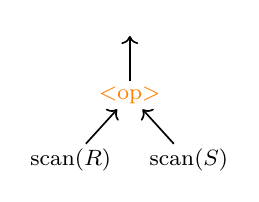
\begin{tikzpicture}[semithick,align=center,node distance=0.825cm,every node/.style={inner sep=1,outer sep=1,font=\footnotesize}]
    \node (0) at (0,0) {};
    \node (1) [below of=0] {\textcolor{orange}{\lstinline{<op>}}};
    \node (2) [below of=1,xshift=-0.75cm] {\lstinline{scan}($R$)};
    \node (3) [below of=1,xshift=0.75cm] {\lstinline{scan}($S$)};

    \path[->]
        (1) edge (0)
        (2) edge (1)
        (3) edge (1);
\end{tikzpicture}
}

%%%%%%%%%%%%%%%%%%%%%%%%%
\begin{frame}{Simplified DBMS architecture}

\begin{center}
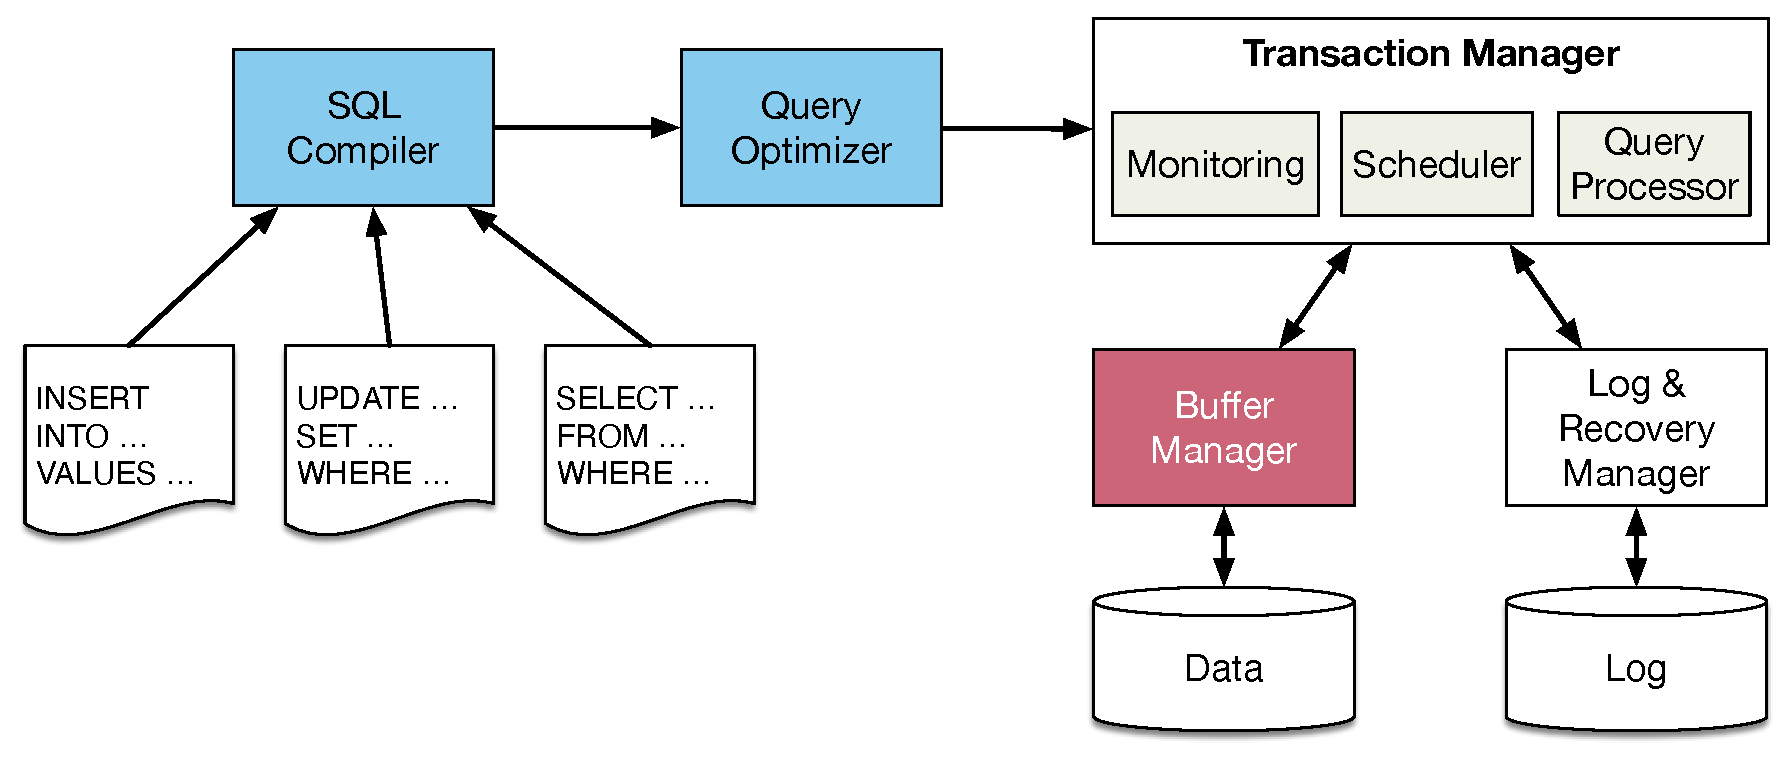
\includegraphics[width=0.8\textwidth]{../lec00_intro/figures/dbms_architecture}
\end{center}

These notes look into algorithms and data structures used to answer relational queries.
\end{frame}

%!TEX root = lec05_query_processing.tex


\begin{frame}

SQL is a \alert{high level declarative language}:
\begin{itemize}[-,noitemsep,topsep=-0.5em]
\item A query specifies \textbf{what} the programmer wants...
\item ... but it does not specify \textbf{how} to compute the answer.
\end{itemize}

\vskip1em

We need to \blue{translate} each SQL query \blue{into} an \blue{an actual executable representation} which the DBMS can process.
\begin{itemize}[-,topsep=-0.5em]
\item Similar to generating executable bytecode from Java.
\end{itemize}

\vskip1em

A \textbf{query plan} is an executable representation of a query.
\begin{itemize}[-,noitemsep,topsep=-0.5em]
\item Query plans, essentially, relational algebra expressions.
\item Recall that we can always translate SQL queries into the algebra because they are equivalent\footnote{Actual implementations of the algebra have operators for advanced SQL features like recursion.}.
\end{itemize}


\end{frame}

%
% --------------------------------------------------------
%

\begin{frame}[fragile]

For example, the SQL query

\begin{center}
\begin{lstlisting}[style=SQL]
SELECT m.director FROM Movie m, Cast c
WHERE m.title=c.title AND m.year=c.year AND
      c.actor='Bill Murray'
\end{lstlisting}
\end{center}

is equivalent to \qquad 
\(\pi_{\texttt{director}} \left(\sigma_{\texttt{actor='Bill Murray'}}
\left(\texttt{\lstinline[style=SQL]{Movie}}\Join\texttt{\lstinline[style=SQL]{Cast}}\right)\right)\)

\vskip2em

\begin{columns}[onlytextwidth]
\begin{column}{0.5\textwidth}
Note that we can represent every algebra expressions as a tree.

\vskip1em

It is common to represent query plans as trees. Most DBMSs have GUIs to let the DBA inspect plans in this way.
\end{column}

\begin{column}{0.5\textwidth}
\begin{center}
\begin{tikzpicture}
    \node (0) at (0,0) {$\pi_{\texttt{director}}$};
    \node (1) [below of=0] {$\sigma_{\texttt{actor='Bill Murray'}}$};
    \node (2) [below of=1] {$\Join$};
    \node (3) [below left of=2] {\lstinline[style=SQL]{Movie}};
    \node (4) [below right of=2] {\lstinline[style=SQL]{Cast}};
    \path[commutative diagrams/.cd, every arrow]
        (4) edge (2)
        (3) edge (2)
        (2) edge (1)
        (1) edge (0);
\end{tikzpicture}
\end{center}
\end{column}
\end{columns}
\end{frame}

%
% --------------------------------------------------------
%

\begin{frame}

The \alert{difference between a plan and an algebra expression} is that the plan specifies \textbf{access methods} are used to read the data and which \textbf{algorithm} is used to implement each operation\footnote{We will see that that are often many choices, especially for joins.}.

\vskip2em

\begin{columns}[onlytextwidth]
\begin{column}{0.5\textwidth}
\begin{center}
\begin{tikzpicture}
    \node (0) at (0,0) {$\pi_{\texttt{director}}$};
    \node (1) [below of=0] {$\sigma_{\texttt{actor='Bill Murray'}}$};
    \node (2) [below of=1] {$\Join$};
    \node (3) [below left of=2] {\lstinline[style=SQL]{Movie}};
    \node (4) [below right of=2] {\lstinline[style=SQL]{Cast}};
    \path[commutative diagrams/.cd, every arrow]
        (4) edge (2)
        (3) edge (2)
        (2) edge (1)
        (1) edge (0);
\end{tikzpicture}
\end{center}
\end{column}

\begin{column}{0.5\textwidth}
\begin{center}
\begin{tikzpicture}
    \node (0) at (0,0) {$\pi_{\texttt{director}}$};
    \node (1) [below of=0] {$\sigma_{\texttt{actor='Bill Murray'}}$};
    \node (2) [below of=1] {\lstinline[style=SQL]{nested_loop_join}};
    \node (3) [below left= 0.35cm and -0.75cm of 2] {\lstinline[style=SQL]{scan(Movie)}};
    \node (4) [below right= 0.35cm and -0.75cm of 2] {\lstinline[style=SQL]{scan(Cast)}};
    \path[commutative diagrams/.cd, every arrow]
        (4) edge (2)
        (3) edge (2)
        (2) edge (1)
        (1) edge (0);
\end{tikzpicture}
\end{center}
\end{column}

\end{columns}

\vskip1em

The \lstinline[style=SQL]{scan()} \textbf{operator} is a full \alert{table scan}, which pulls tuples from a table file (heap or sequential).
\end{frame}

%
% --------------------------------------------------------
%


\begin{frame}{The life cycle of a query}
\begin{tikzpicture}
\node at (0,0) [anchor=south west] {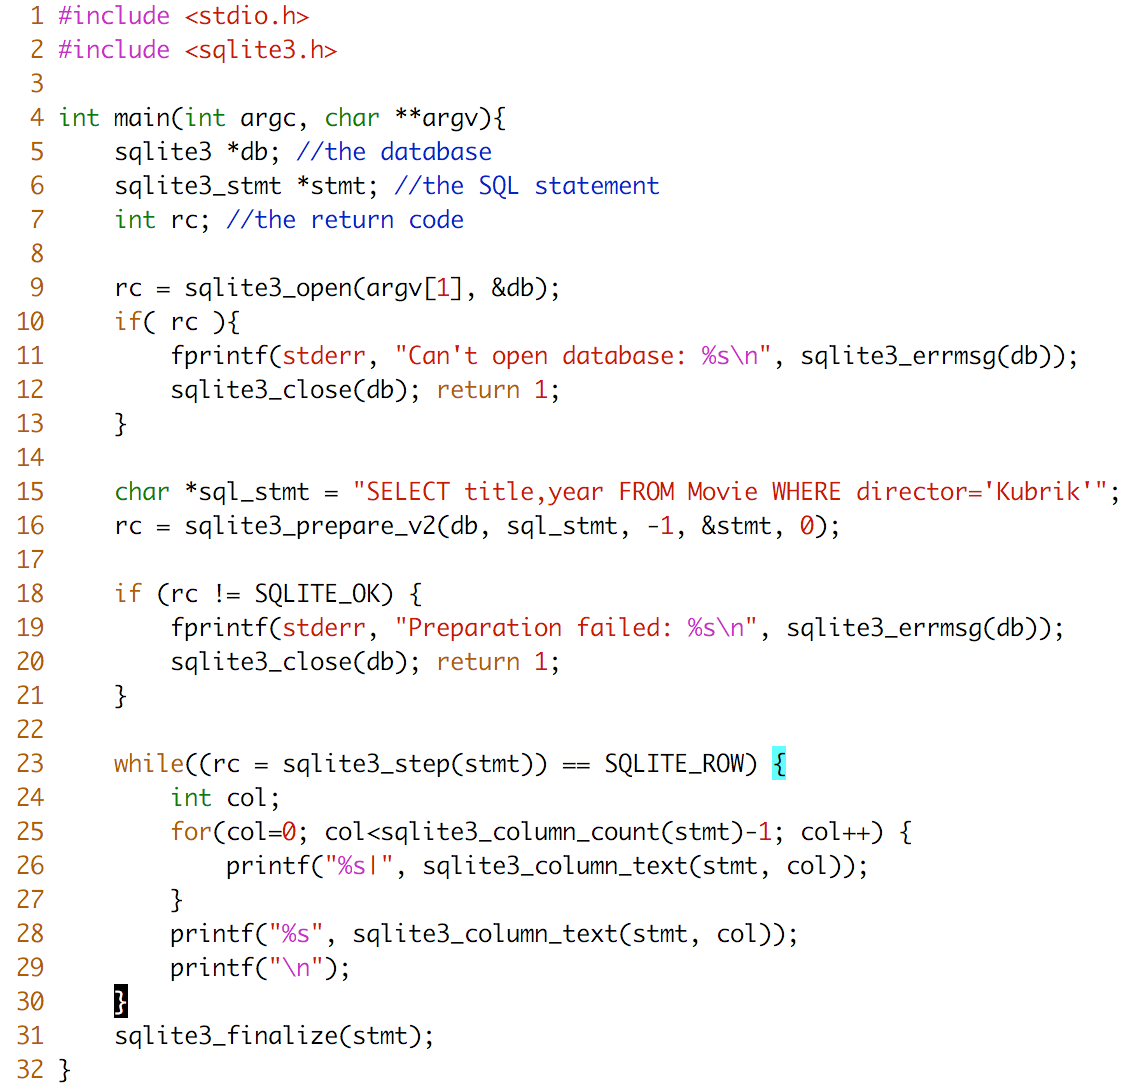
\includegraphics[width=0.75\textwidth]{figures/sample_C_program}};
\coordinate (prepare) at (6.125,4.125);
\coordinate (fetch) at (3.5,2.525);

\only<2-3>\node (compile) [color=fern,draw] at (9.5,5.125) {\begin{minipage}{2.75cm}
\fontsize{8}{9}\selectfont \centering compile SQL query\\
into (algebraic) plan \end{minipage}};
\only<2-3>\draw [->,color=fern] (compile) to[out=270,in=0] (prepare);

\only<3>\node (step) [color=fern,draw] at (9.5,2.65) {\begin{minipage}{2.75cm}
\fontsize{8}{9}\selectfont \centering fetch tuples\\
one-at-a-time \end{minipage}};
\only<3>\draw [->,color=fern] (step) to[out=180,in=45] (fetch);
\end{tikzpicture}
\end{frame}



\begin{frame}

\textbf{Compiling} the SQL query

\begin{center}
\fbox{\clipbox{0pt 110pt 0pt 95pt}{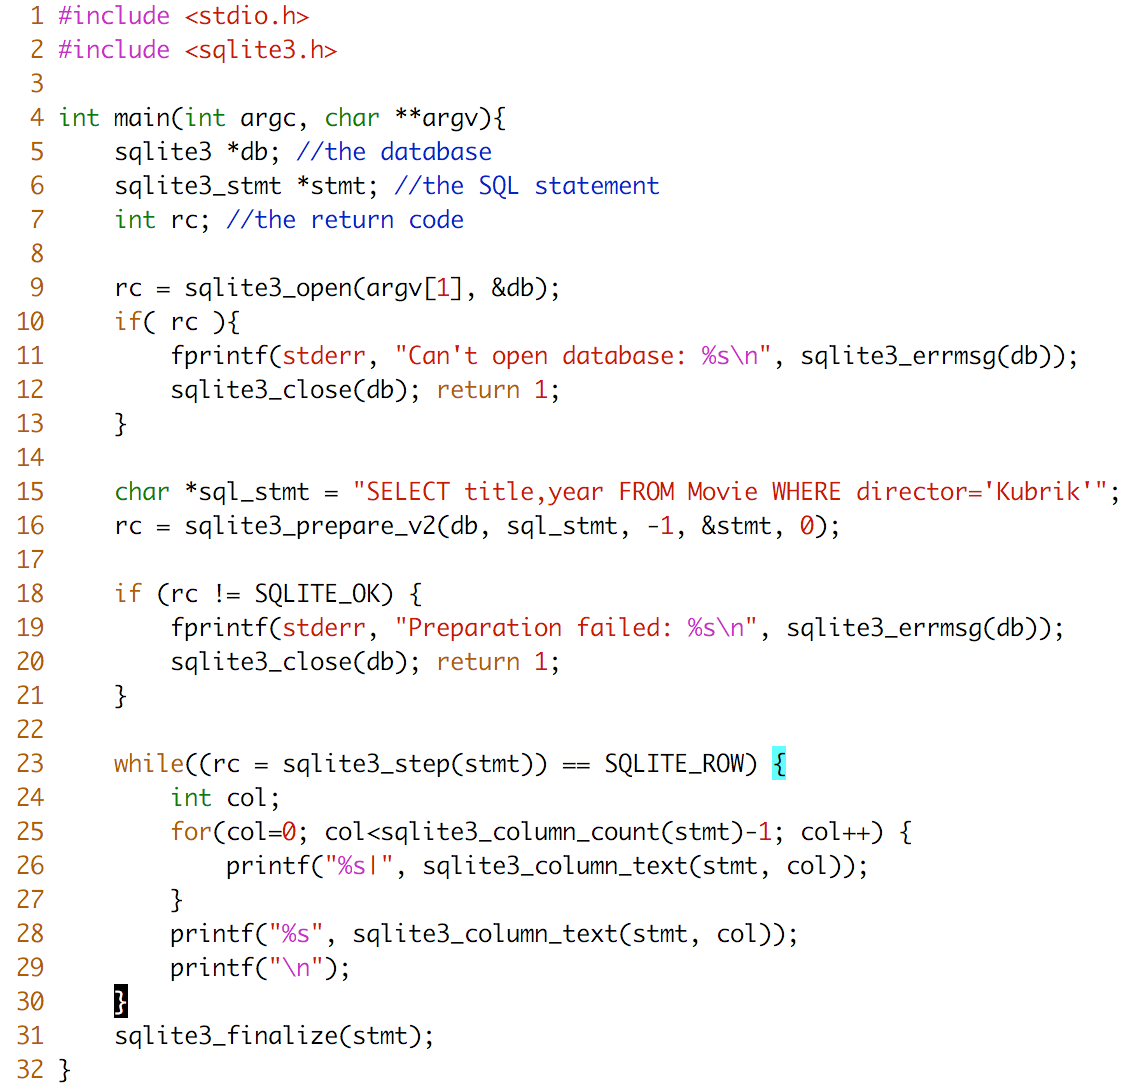
\includegraphics[width=0.75\textwidth]{figures/sample_C_program}}}
\end{center}

\vskip1em

... produces a query plan looking like this:

\vskip1em

\begin{center}
	\begin{tikzpicture}[align=center,node distance=0.825cm,every node/.style={inner sep=1,outer sep=1}]
    \node (P1) at (0,0) {$\pi_{\texttt{title,year}}$};
    \node (P2) [below of=P1] {$\sigma_{\texttt{director='Kubrick'}}$};
    \node (P3) [below of=P2] {\lstinline[style=SQL]{scan(Movie)}};
    \path[->] 
    	(P2) edge (P1)
        (P3) edge (P2);
\end{tikzpicture}
\end{center}

\end{frame}



\begin{frame}

The query plan is executed \textbf{iteratively}:

Every call to \lstinline[style=SQL]{sqlite3_step()} fetches \textbf{one \alert{new} tuple} of the answer, and stores it in the heap space of the application.

\vskip1em

\begin{center}
\fbox{\clipbox{0pt 15pt 0pt 150pt}{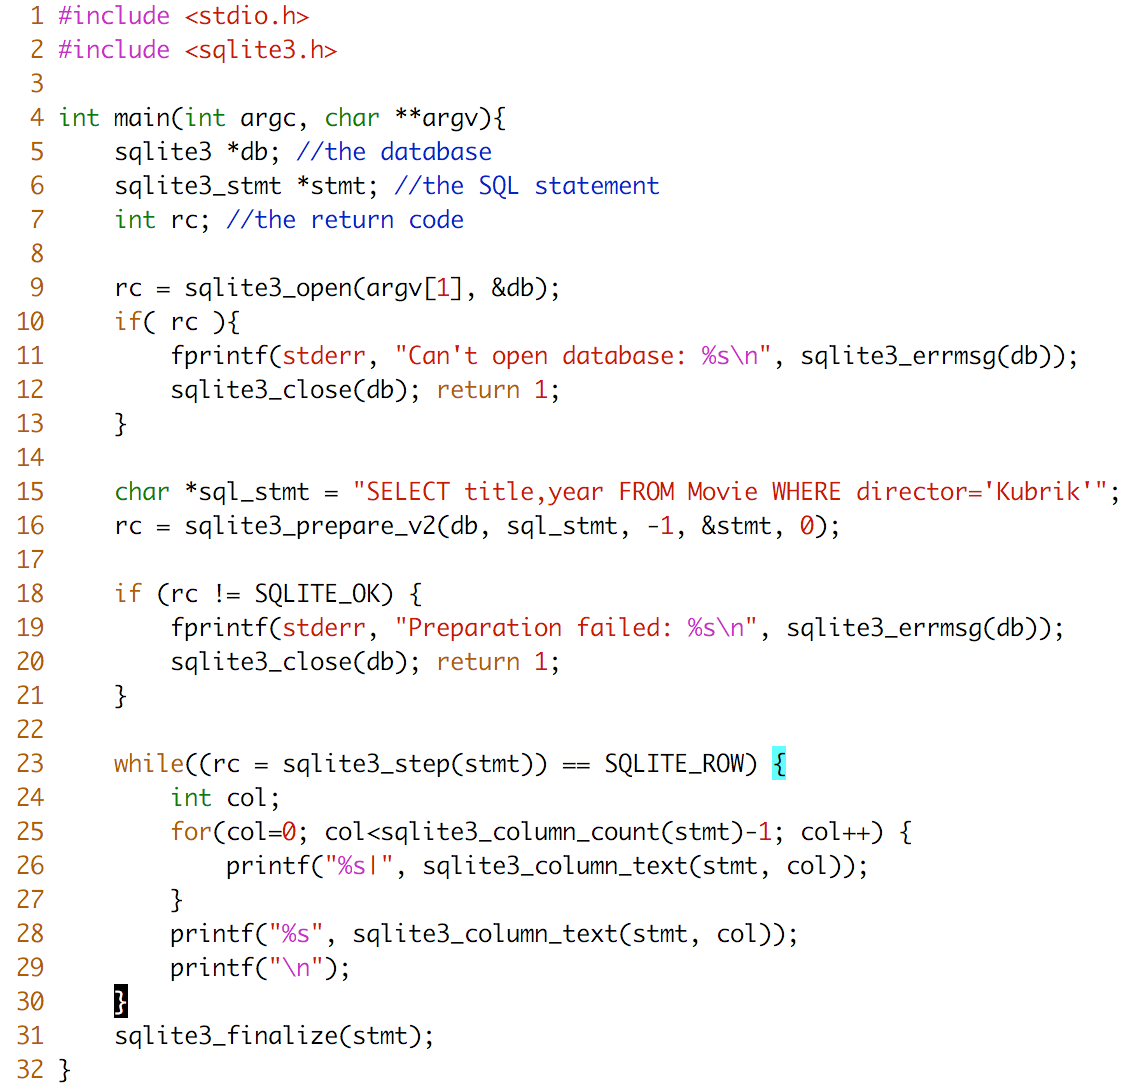
\includegraphics[width=0.75\textwidth]{figures/sample_C_program}}}
\end{center}

\vskip1em

\lstinline[style=SQL]{sqlite3_step()} has a specific return code to indicate that all tuples in the answer have already been fetched.

\end{frame}

\begin{frame}

\vskip0.75em

\textbf{How is a call to \lstinline[style=SQL]{sqlite3_step()} executed?}

\vskip0.75em

Every node in the query plan implements an interface defining the \lstinline[style=SQL]{getNext()} method, which must returns \alert{a tuple that has not been returned \textbf{by that node} before}.

\vskip1em

\begin{center}
	\begin{tikzpicture}[align=center,node distance=0.825cm,every node/.style={inner sep=1,outer sep=1}]
    \node (P1) at (0,0) {$\pi_{\texttt{title,year}}$};
    \node (P2) [below of=P1] {$\sigma_{\texttt{director='Kubrick'}}$};
    \node (P3) [below of=P2] {\lstinline[style=SQL]{scan(Movie)}};
    \path[->]
    	(P2) edge (P1)
        (P3) edge (P2);

    \pause
    \node (step1) [right=2cm of P1] {\lstinline[style=SQL]{getNext()}};
    \node (app_step) [above of=step1] {\lstinline[style=SQL]{sqlite3_step()}};
    \draw[->,red] ($(app_step)-(0.5,0.175)$) -- ($(step1)-(0.5,-0.175)$);

    \pause
    \node (step2) [below of=step1] {\lstinline[style=SQL]{getNext()}};
    \draw[->,red] ($(step1)-(0.5,0.175)$) -- ($(step2)-(0.5,-0.175)$);

    \pause
    \node (step3) [below of=step2] {\lstinline[style=SQL]{getNext()}};        
    \draw[->,red] ($(step2)-(0.5,0.175)$) -- ($(step3)-(0.5,-0.175)$);

    \pause
    \draw[->,blue] ($(step3)+(0.5,0.175)$) -- ($(step2)+(0.5,-0.175)$);

    \pause
    \draw[->,blue] ($(step2)+(0.5,0.175)$) -- ($(step1)+(0.5,-0.175)$);

    \pause
    \draw[->,blue] ($(step1)+(0.5,0.175)$) -- ($(app_step)+(0.5,-0.175)$);

\end{tikzpicture}
\end{center}

\vskip2em

\lstinline[style=SQL]{sqlite3_step()} calls \lstinline[style=SQL]{getNext()} on the root node of the plan, which leads to further calls to the nodes below, until a new tuple is returned to the application.

\end{frame}


\begin{frame}[fragile]

Those objects returning the ``next tuple'' are called \textbf{iterators}. The DBMS implements at lest one iterator for each kind of operator in the query plan. 

\vskip1em

The DBMS might have different iterators with different algorithms for the same operator. At query optimization time, the DBMS must decide which iterator to use based on the cost of the corresponding algorithm and the available resources.

\vskip1em

Iterators are \textbf{stateful} objects: they cannot return the same tuple more than once, so they need to somehow remember which ones were already returned.
\begin{itemize}[-,topsep=-0.5em]
\item Iterators return \alert{\textbf{\lstinline[style=SQL]{<EOF>}} (end of file)} when there are no more tuples to be returned.
\end{itemize}
 

\end{frame}
\tableofcontents

%%%%%%%%%% ------------------------

\section{Query Compilation}
%!TEX root = lec05_query_processing.tex


%
% --------------------------------------------------------------------------------------------------------------------------------------
%
\begin{frame}[fragile]{Compiling SQL into algebra expressions}

Recap: 

\begin{itemize}[-]
\item SQL is a complex language, with many sophisticated constructs that are beyond our scope here. Instead we focus on the basic building blocks.

\item \alert{A query plan is, essentially, an algebra expression} with access methods instead of table names.

\item The main difference between a plan and a ``pure'' algebra expression is that in the plan we need to specify the access methods we use to read the database.
\end{itemize}

\end{frame}


\newsavebox\algebraBasicSelectFromWhere
\savebox{\algebraBasicSelectFromWhere}{
    \begin{tikzpicture}[align=center,node distance=0.825cm,every node/.style={inner sep=1,outer sep=1,font=\footnotesize}]
    \node (P1) at (0,0) {$\pi_{a_1,\ldots,a_n}$};
    \node (P2) [below of=P1] {$\sigma_{c_1\ \wedge\ \cdots\ \wedge c_k}$};
    \node (P3) [below of=P2] {$\times$};
    \node (P4) [below left=0.25cm and 0.25cm of P3] {$\times$};
    \node (P5) [below right=0.25cm and 0.25cm of P3] {$T_m$};
    \node (P6) [below right=0.25cm and 0.25cm of P4] {$T_{m-1}$};
    \node (P7) [inner sep=4,below left=0.25cm and 0.125cm of P4] {$\cdots$};
    \node (P8) [below left=0.25cm and 0.125cm of P7] {$\times$};
    \node (P9) [below left=0.25cm and 0.125cm of P8] {$T_1$};
    \node (P10) [below right=0.25cm and 0.125cm of P8] {$T_2$};
    \path[commutative diagrams/.cd, every arrow]
        (P2) edge (P1)
        (P3) edge (P2)
        (P4) edge (P3)
        (P5) edge (P3)
        (P6) edge (P4)
        (P7) edge (P4)
        (P8) edge (P7)
        (P9) edge (P8)
        (P10) edge (P8);
\end{tikzpicture}%
}

%
% --------------------------------------------------------------------------------------------------------------------------------------
%
\begin{frame}[fragile]{Compiling basic SQL expressions}

\begin{columns}[onlytextwidth]
\begin{column}{0.5\textwidth}

The basic compilation step translates a \textbf{conjunctive SQL query} into a ``\alert{\textbf{canonical}}'' plan like:

\vskip1em

\begin{lstlisting}[style=SQL,escapeinside={(*}{*)},frame=single]
SELECT (*$a_1, a_2, \ldots, a_n$*)
FROM (*$T_1$*) [, (*$T_2$*) [, (*$\ldots$*) [, (*$T_m$*)]]]
WHERE (*$c_1$*) AND (*$c_2$*) AND (*\ldots*) AND (*$c_k$*)
\end{lstlisting}
\end{column}

\vspace*{-2.5em}
\begin{column}{0.45\textwidth}
\usebox\algebraBasicSelectFromWhere
\end{column}
\end{columns}

\vskip2em

If there is a single table expression\\ in the query, we omit the Cartesian product of course.

We omit the \lstinline[style=SQL]{scan()} operators here for simplicity.

\end{frame}


%
% --------------------------------------------------------------------------------------------------------------------------------------
%
\begin{frame}[fragile]

The \alert{\emph{renaming operator} $\rho()$} is used to handle the tuple variable declarations in SQL.


\vskip3em

\begin{columns}
\begin{column}{0.5\textwidth}
\begin{lstlisting}[style=SQL,frame=single]
SELECT m.title, m.year
FROM Movie -:m:-
WHERE m.director = 'Ivan Reitman'
\end{lstlisting}
\end{column}
\begin{column}{0.4\textwidth}
\begin{tikzpicture}[align=center,node distance=0.825cm,every node/.style={inner sep=1,outer sep=1,font=\footnotesize}]
\node (pi) at (0,0) {$\pi_{\texttt{m.title, m.year}}$};
\node (sigma) [below of=pi] {$\sigma_{\texttt{m.director='Ivan Reitman'}}$};
\node (rho) [below of=sigma] {$\rho_{\texttt{\lstinline[style=SQL]{-:m:-}(m.title, m.year, m.imdb, m.director)}}$};
\node (Movie) [below of=rho] {\lstinline[style=SQL]!scan(Movie)!};
\path[->]
	(Movie) edge (rho)
	(rho) edge (sigma)
	(sigma) edge (pi);
\end{tikzpicture}
\end{column}
\end{columns}
\end{frame}

%
% --------------------------------------------------------------------------------------------------------------------------------------
%

\newsavebox\bmmMovieCrossProduct
\savebox{\bmmMovieCrossProduct}{
    \begin{tikzpicture}[align=center,node distance=0.825cm,every node/.style={inner sep=1,outer sep=1,font=\footnotesize}]
    \node (P1) at (0,0) {$\pi_{\texttt{m.director}}$};
    \node (P2) [below of=P1] {$\sigma_{\substack{\texttt{m.year=bmm.year}\\\wedge\ \texttt{m.title=bmm.title}}}$};
    \node (P3) [below of=P2] {$\times$};
    \node (P4) [below of=P3,xshift=1.5cm] {$\rho_{\substack{\texttt{bmm(bmm.title,}\\%
           \texttt{bmm.year)}}}$};
    \node (P5) [below of=P3,xshift=-1cm] {$\rho_{\substack{\texttt{m(m.title, m.year}\\
           \texttt{m.imdb,m.director)}}}$};
    \node (P6) [below=0.5cm of P4] {$\pi_{\texttt{title,year}}$};           
    \node (P7) [below=0.5cm of P6] {$\sigma_{\texttt{actor='Bill Murray'}}$};
    \node (P8) [below=0.5cm of P7] {\lstinline[style=SQL]!scan(Cast)!};
    \node (P9) [below=0.5cm of P5] {\lstinline[style=SQL]!scan(Movie)!};
    \path[commutative diagrams/.cd, every arrow]
        (P2) edge (P1)
        (P3) edge (P2)
        (P4) edge (P3)
        (P5) edge (P3)
        (P6) edge (P4)
        (P7) edge (P6)
        (P8) edge (P7)
        (P9) edge (P5);
\end{tikzpicture}}


\newsavebox\bmmMovieJoin
\savebox{\bmmMovieJoin}{
    \begin{tikzpicture}[align=center,node distance=0.825cm,every node/.style={inner sep=1,outer sep=1,font=\footnotesize}]
    \node (P1) at (0,0) {$\pi_{\texttt{m.director}}$};
    \node (P3) [below of=P1] {$\Join_{\substack{\texttt{m.year=bmm.year}\\\wedge\ \texttt{m.title=bmm.title}}}$};
    \node (P4) [below of=P3,xshift=1.5cm] {$\rho_{\substack{\texttt{bmm(bmm.title,}\\%
           \texttt{bmm.year)}}}$};
    \node (P5) [below of=P3,xshift=-1cm] {$\rho_{\substack{\texttt{m(m.title, m.year}\\
           \texttt{m.imdb,m.director)}}}$};
    \node (P6) [below=0.5cm of P4] {$\pi_{\texttt{title,year}}$};           
    \node (P7) [below=0.5cm of P6] {$\sigma_{\texttt{actor='Bill Murray'}}$};
    \node (P8) [below=0.5cm of P7] {\lstinline[style=SQL]!scan(Cast)!};
    \node (P9) [below=0.5cm of P5] {\lstinline[style=SQL]!scan(Movie)!};
    \path[commutative diagrams/.cd, every arrow]
        (P3) edge (P1)
        (P4) edge (P3)
        (P5) edge (P3)
        (P6) edge (P4)
        (P7) edge (P6)
        (P8) edge (P7)
        (P9) edge (P5);
\end{tikzpicture}}

\begin{frame}[fragile]

Table expressions given as SQL queries are translated into \textbf{sub-expressions} ``below the Cartesian product'' in the main plan:

\vskip2em

\begin{columns}
\begin{column}{0.425\textwidth}
\begin{lstlisting}[style=SQL,frame=single]
SELECT m.director
FROM Movie m, 
  (SELECT title, year 
   FROM Cast
   WHERE actor='Bill Murray'
  ) AS bmm
WHERE m.year=bmm.year 
  AND m.title=bmm.title;
\end{lstlisting}
\end{column}
\begin{column}{0.4\textwidth}
% \vspace*{-2em}
\usebox{\bmmMovieCrossProduct}
\end{column}
\end{columns}
\end{frame}

%
% --------------------------------------------------------------------------------------------------------------------------------------
%
\begin{frame}

It is OK to ``\textbf{\alert{push down}}'' conditions in the \lstinline[style=SQL]{WHERE} clause that define a join, replacing the Cartesian product when possible:


\vskip2em

\begin{columns}
\begin{column}{0.425\textwidth}
\scalebox{0.9}{\usebox{\bmmMovieCrossProduct}}
\end{column}
\begin{column}{0.4\textwidth}
\usebox{\bmmMovieJoin}
\end{column}
\end{columns}


\end{frame}


%
% --------------------------------------------------------------------------------------------------------------------------------------
%
\begin{frame}[fragile]

Set/bag operators are also translated into their algebra counterparts:

\textbf{Example:}

\begin{columns}
\begin{column}{0.425\textwidth}
\begin{lstlisting}[style=SQL,frame=single]
SELECT title, year
FROM Cast
WHERE actor="Bill Murray"
INTERSECT
SELECT title, year 
FROM Movie
WHERE imdb>7
\end{lstlisting}
\end{column}
\begin{column}{0.4\textwidth}
\begin{tikzpicture}[align=center,node distance=0.825cm,every node/.style={inner sep=1,outer sep=1,font=\footnotesize}]
    \node (intersection) at (0,0) {$\cap_{\text{distinct}}$};
    \node (sub1) [below of=intersection,xshift=-1cm] {$\pi_{\texttt{title,year}}$};
    \node (sub2) [below of=intersection,xshift=1cm] {$\pi_{\texttt{title,year}}$};
    \node (sigma1) [below of=sub1] {$\sigma_{\texttt{actor='Bill Murray'}}$};
    \node (Cast) [below of=sigma1] {\lstinline[style=SQL]!scan(Cast)!};
    \node (sigma2) [below of=sub2] {$\sigma_{\texttt{imdb>7}}$};
    \node (Movie) [below of=sigma2] {\lstinline[style=SQL]!scan(Movie)!};
    \path[->]
        (Cast) edge (sigma1)
        (sigma1) edge (sub1)
        (sub1) edge (intersection)
        (Movie) edge (sigma2)
        (sigma2) edge (sub2)
        (sub2) edge (intersection);
\end{tikzpicture}
\end{column}
\end{columns}
\end{frame}


%
% --------------------------------------------------------------------------------------------------------------------------------------
%
\begin{frame}[fragile]
Aggregation is handled by operator \(\gamma_{\text{<grouping>,fn()}}(R)\)

\vskip0.5em

The \lstinline[style=SQL]{GROUP BY} clause goes into ``grouping'' and \lstinline[style=SQL]{fn()} is the set function. The \lstinline[style=SQL]{HAVING} clause are handled with a selection.

\vskip2em

\begin{columns}
\begin{column}{0.4\textwidth}
\begin{lstlisting}[style=SQL,frame=single]
SELECT theater, COUNT(*) 
FROM Guide
WHERE start > 1100
GROUP BY theater
HAVING COUNT(*) > 4
\end{lstlisting}
\end{column}
\begin{column}{0.3\textwidth}
\scalebox{1}{
     \begin{tikzpicture}[align=center,node distance=0.825cm,every node/.style={inner sep=0.5,outer sep=0.5,font=\footnotesize}]
    \node (P1) at (0,0) {$\pi_{\text{theater, COUNT(*)}}$};
    \node (P2) [below of=P1] {$\sigma_{\texttt{COUNT(*)}>4}$};
    \node (P3) [below of=P2] {$\gamma_{\texttt{theater, COUNT(*)}}$};
    \node (P4) [below of=P3] {$\sigma_{\texttt{start}>1100}$};
    \node (P5) [below of=P4] {\lstinline[style=SQL]!scan(Guide)!};
    \path[->]
        (P2) edge (P1)
        (P3) edge (P2)
        (P4) edge (P3)
        (P5) edge (P4);
\end{tikzpicture}%
}
\end{column}
\end{columns}
\end{frame}


%
% --------------------------------------------------------------------------------------------------------------------------------------
%
\begin{frame}[fragile]{Sub-Queries in Other Expressions}

Recall SQL allows sub-queries to appear inside value expressions and in predicates in the \lstinline[style=SQL]{WHERE} clause.

\vskip2em

\begin{columns}[onlytextwidth]
\begin{column}{0.4\textwidth}
\begin{lstlisting}[style=SQL]
SELECT 100 + (
        SELECT COUNT(*)
        FROM Movie
       );
\end{lstlisting}
\end{column}
\begin{column}{0.5\textwidth}
\begin{lstlisting}[style=SQL]
SELECT m.title 
FROM Movie m
WHERE m.imdb = (SELECT MAX(imdb)
                FROM Movie);
\end{lstlisting}
\end{column}
\end{columns}

\vskip2em


Actual query plans in production DBMSs have nodes beyond the relational algebra (e.g., to handle complex arithmetic or string operations from the results of sub-queries).
\end{frame}

\newsavebox{\preprocessorCTEexample}
\begin{lrbox}{\preprocessorCTEexample}
\begin{minipage}{0.5\textwidth}
\begin{lstlisting}[style=SQL]
WITH TopMovie(title, year) AS (
    SELECT title, year 
    FROM Movie WHERE imdb > 7
)
SELECT c.role
FROM Cast c, TopMovie tm
WHERE c.title=tm.title AND 
      c.year=tm.year AND
      c.actor="Sigourney Weaver";
\end{lstlisting}
\end{minipage}
\end{lrbox}

\newsavebox{\preprocessorCTEexampleRewritten}
\begin{lrbox}{\preprocessorCTEexampleRewritten}
\begin{minipage}{0.5\textwidth}
\begin{lstlisting}[style=SQL,escapechar=|]
SELECT c.role
FROM Cast c, |\alert{(}|
    |\alert{SELECT title, year}| 
    |\alert{FROM Movie WHERE imdb > 7}|
    |\alert{) AS tm}|
WHERE c.title=tm.title AND 
      c.year=tm.year AND
      c.actor="Sigourney Weaver";
\end{lstlisting}
\end{minipage}
\end{lrbox}

%
% --------------------------------------------------------------------------------------------------------------------------------------
%
\begin{frame}[fragile]{The SQL Preprocessor}

Other constructs in SQL such as \emph{views} and Common Table Expressions (CTEs) given through \lstinline[style=SQL]{WITH} clauses are handled by the SQL \textbf{preprocessor}.

Views and non-recursive CTEs are treated essentially as \emph{macros} in a C program: the preprocessor replaces every occurrence of the CTE or the view in a table expression by that CTE/view definition:

\vskip1em

\begin{columns}
\begin{column}{0.4\textwidth}
\scalebox{0.75}{\usebox\preprocessorCTEexample}
\end{column}
\begin{column}{0.4\textwidth}
\scalebox{0.75}{\usebox\preprocessorCTEexampleRewritten}
\end{column}
\end{columns}
\end{frame}


%%%%%%%%%%%%%%%% ------------------------

\section{The Iterator Model}
%!TEX root = lec05_query_processing.tex

%
% -------------------------------------------
%
\newsavebox\iteratorExampleTree
\savebox{\iteratorExampleTree}{
\begin{tikzpicture}[semithick,align=center,node distance=0.875cm,every node/.style={inner sep=1,outer sep=1,font=\footnotesize}]
% \node (0) at (0,0) {} ; %empty node with ``answer''
\node (1) at (0,0) {$\pi_{\texttt{role,imdb}}$};
\node (3) [below of= 1] {$\Join$};
\node (4) [below left of= 3, xshift=-0.25cm] {\lstinline[style=SQL]!scan(Movie)!};
\node (2) [below right of= 3, xshift=0.25cm, yshift=-0.75cm] {$\sigma_{\texttt{actor='Bill Murray'}}$};
\node (5) [below of =2] {\lstinline[style=SQL]!scan(Cast)!};
\path[->]
    (4) edge (3)
    (5) edge (2) 
    (3) edge (1)
    (2) edge (3);
    % (1) edge (0);
\end{tikzpicture}
}

%
% -------------------------------------------
%
\begin{frame}{The Iterator Interface}

All nodes in a query plan must implement the following three methods:


\begin{columns}[onlytextwidth]
\begin{column}{0.6\textwidth}
\begin{itemize}[label=$\circ$]
\item \textbf{Open()}:  creates/requests the necessary data structures.
\item \textbf{GetNext()}:  produces \alert{\textbf{the} next tuple} for that node.
\item \textbf{Close()}:  releases the necessary data structures.
\end{itemize}


\end{column}
\begin{column}{0.4\textwidth}
\flushright
\usebox\iteratorExampleTree
\end{column}
\end{columns}

\vskip1em

\begin{block}{\alert{\textbf{Remember this}}}
Each call to \textbf{GetNext()} \alert{produces just one tuple}: the next tuple that the node must return.
\end{block}

\end{frame}


%
% -------------------------------------------
%
\begin{frame}{Open()/Close()}
\vskip1em
\begin{columns}[onlytextwidth]
\begin{column}{0.6\textwidth}
\textbf{Open()} is called recursively, top-down, from the root of the tree

\vskip0.5em

A call to \textbf{Open()} is supposed to:

\vskip0.5em

\begin{enumerate}[label=(\arabic*)]
\item create any necessary input buffers
\item initialize any variables needed (ex: pointers to tuples in a nested loop join operator)
\item open a file if the operator is a table or index scan
\end{enumerate}

\vskip1em

The analogous \textbf{Close()} method frees up all those resources.

\end{column}
\begin{column}{0.4\textwidth}
\qquad\qquad
\begin{tikzpicture}[semithick,align=center,node distance=0.875cm,every node/.style={inner sep=1,outer sep=1,font=\footnotesize}]
\node[anchor=north,inner sep=0pt,outer sep=0pt] at (0,0) {\scalebox{1}{\usebox{\iteratorExampleTree}}};

\node (0) at (-1.5,-0.125) [color=red] {Open()};
\pause
\node (1) [below of=0,color=red] {Open()};
\draw [->, color=red] (0) -- (1);
\pause
\node (2) [below of=1,xshift=-0.75cm,yshift=0.125cm,,color=red] {Open()};
\draw [->, color=red] (1) -- (2);
\pause
\node (3) [below of=1,xshift=0.4cm, yshift=-0.5cm,color=red] {Open()};
\draw [->, color=red] (1) -- (3);
\pause
\node (4) [below of=3,color=red] {Open()};
\draw [->, color=red] (3) -- (4);
\end{tikzpicture}
\end{column}
\end{columns}

\end{frame}


%
% -------------------------------------------
%
\begin{frame}{GetNext()}

\vskip1em

\begin{columns}[onlytextwidth]
\begin{column}{0.55\textwidth}

\textbf{GetNext()} computes \alert{one more tuple} and returns it to the operator ``above'' it in the plan.

\vskip1em

\textbf{GetNext()} returns \alert{\lstinline[style=SQL]{<EOF>}} when there are no more tuples to return.

\end{column}
\begin{column}{0.4\textwidth}
\flushright
\begin{tikzpicture}[semithick,align=center,node distance=0.875cm,every node/.style={inner sep=1,outer sep=1,font=\footnotesize}]
\node[anchor=north,inner sep=0pt,outer sep=0pt] at (0,0) {\scalebox{1}{\usebox{\iteratorExampleTree}}};
\node (0) at (-1.5,-0.125) [color=red] {GetNext()};
\pause
\node (1) [below of=0,color=red] {GetNext()};
\draw [->, color=red,transform canvas={xshift=-2pt}] (0) -- (1);
\pause
\node (2) [below of=1,xshift=-0.75cm,yshift=0.125cm,,color=red] {GetNext()};
\draw [->, color=red,transform canvas={xshift=-2pt}] (1) -- (2);
\pause
\draw [->,color=blue,transform canvas={xshift=2pt}] (2) -- (1);
\pause
\node (3) [below of=1,xshift=0.4cm, yshift=-0.5cm,color=red] {GetNext()};
\draw [->, color=red,transform canvas={xshift=-2pt}] (1) -- (3);
\pause
\node (4) [below of=3,color=red] {GetNext()};
\draw [->, color=red,transform canvas={xshift=-2pt}] (3) -- (4);
\pause
\draw [->,color=blue,transform canvas={xshift=2pt}] (4) -- (3);
\pause
\draw [->,color=blue,transform canvas={xshift=2pt}] (3) -- (1);
\pause
\draw [->,color=blue,transform canvas={xshift=2pt}] (1) -- (0);
\pause
\draw [->,color=blue,transform canvas={xshift=2pt}] (0) -- (-1.5,0.5);
\end{tikzpicture}
\end{column}
\end{columns}

\end{frame}

\begin{frame}
\begin{columns}[onlytextwidth]
\begin{column}{0.6\textwidth}
\alert{scan(R)}: returns next tuple from $R$, reading a new block from disk if needed.

\vskip2em

\alert{$\pi_{a_1,\ldots,a_n}(R)$}: calls \lstinline[style=SQL]{getNext()} on operator below, strip unwanted attributes and return the resulting tuple
\end{column}
\begin{column}{0.4\textwidth}
\flushright
\begin{tikzpicture}[semithick,align=center,node distance=0.875cm,every node/.style={inner sep=1,outer sep=1,font=\footnotesize}]
\node[anchor=north,inner sep=0pt,outer sep=0pt] at (0,0) {\scalebox{1}{\usebox{\iteratorExampleTree}}};
\node (0) at (-1.5,-0.125) [color=red] {GetNext()};
\node (1) [below of=0,color=red] {GetNext()};
\draw [->, color=red,transform canvas={xshift=-2pt}] (0) -- (1);
\node (2) [below of=1,xshift=-0.75cm,yshift=0.125cm,,color=red] {GetNext()};
\draw [->, color=red,transform canvas={xshift=-2pt}] (1) -- (2);
\draw [->,color=blue,transform canvas={xshift=2pt}] (2) -- (1);
\node (3) [below of=1,xshift=0.4cm, yshift=-0.5cm,color=red] {GetNext()};
\draw [->, color=red,transform canvas={xshift=-2pt}] (1) -- (3);
\node (4) [below of=3,color=red] {GetNext()};
\draw [->, color=red,transform canvas={xshift=-2pt}] (3) -- (4);
\draw [->,color=blue,transform canvas={xshift=2pt}] (4) -- (3);
\draw [->,color=blue,transform canvas={xshift=2pt}] (3) -- (1);
\draw [->,color=blue,transform canvas={xshift=2pt}] (1) -- (0);
\draw [->,color=blue,transform canvas={xshift=2pt}] (0) -- (-1.5,0.5);\end{tikzpicture}
\end{column}
\end{columns}
\end{frame}


%
% -------------------------------------------
%
\begin{frame}
\begin{columns}[onlytextwidth]
\begin{column}{0.6\textwidth}
\alert{$\sigma_{C}(R)$}: \underline{repeatedly} calls \lstinline[style=SQL]{getNext()} on operator below until a tuple that satisfies the condition $C$ is found; returning that tuple (or \lstinline[style=SQL]{<EOF>} if no such tuple exists).

\vskip2em

\alert{$R \Join_{C} S$}: calls \lstinline[style=SQL]{getNext()} on iterators for $R$ and $S$ according to the algorithm, until a match is found.

\end{column}
\begin{column}{0.4\textwidth}
\flushright
\begin{tikzpicture}[semithick,align=center,node distance=0.875cm,every node/.style={inner sep=1,outer sep=1,font=\footnotesize}]
\node[anchor=north,inner sep=0pt,outer sep=0pt] at (0,0) {\scalebox{1}{\usebox{\iteratorExampleTree}}};
\node (0) at (-1.5,-0.125) [color=red] {GetNext()};
\node (1) [below of=0,color=red] {GetNext()};
\draw [->, color=red,transform canvas={xshift=-2pt}] (0) -- (1);
\node (2) [below of=1,xshift=-0.75cm,yshift=0.125cm,,color=red] {GetNext()};
\draw [->, color=red,transform canvas={xshift=-2pt}] (1) -- (2);
\draw [->,color=blue,transform canvas={xshift=2pt}] (2) -- (1);
\node (3) [below of=1,xshift=0.4cm, yshift=-0.5cm,color=red] {GetNext()};
\draw [->, color=red,transform canvas={xshift=-2pt}] (1) -- (3);
\node (4) [below of=3,color=red] {GetNext()};
\draw [->, color=red,transform canvas={xshift=-2pt}] (3) -- (4);
\draw [->,color=blue,transform canvas={xshift=2pt}] (4) -- (3);
\draw [->,color=blue,transform canvas={xshift=2pt}] (3) -- (1);
\draw [->,color=blue,transform canvas={xshift=2pt}] (1) -- (0);
\draw [->,color=blue,transform canvas={xshift=2pt}] (0) -- (-1.5,0.5);\end{tikzpicture}
\end{column}
\end{columns}
\end{frame}

%
% -------------------------------------------
%
\begin{frame}{Iterators for other binary operators}

The iterators for \alert{$R - S$}, \alert{$R \cup S$} and \alert{$R \cap S$} are analogous to \alert{$R \Join_{C} S$} and make repeated calls to \lstinline[style=SQL]{getNext()} on the iterators for $R$ and $S$ to obtain tuples from each sub-expression.

\vskip2em

We will look at intricacies of the algorithms later in these slides.


\end{frame}


%
% -------------------------------------------
%
\begin{frame}[fragile]

The next slides show naive (and incomplete) Python-like implementations of some of the iterators, focusing on semantics\footnote{After we look at the I/O cost analysis of simple query plans, we will discuss better algorithms for the iterators.} but omitting details. 

\vskip1em

Assume there is an interface, called \lstinline[style=Python]{Iterator}, declaring all operations that each iterator must implement.
\begin{itemize}[-,topsep=-5pt,noitemsep]
\item For simplicity, we omit details like constructors.
\item \lstinline[style=Python]{Iterator.from(X)} compiles relational expression \lstinline[style=Python]{X} into the appropriate iterator object.
\end{itemize}

\vskip1em



\end{frame}

%
% -------------------------------------------
%
\begin{frame}[fragile]{Iterator for $\sigma_C(R)$ }

\begin{lstlisting}[style=Python,multicols=2]
Class Selection(Iterator):

  def Open():
    self.i = Iterator.from(self.R)
    self.i.Open()


  def Close():
    self.i.Close()


  def GetNext():
    # read tuple from R
    t = self.i.GetNext() 
    while t !=  EOF and 
        not satisfies(t, self.C):
      t = i.GetNext()
    yield t

\end{lstlisting}


\vskip0.25em

\begin{block}{}%{Iterator state}
The selection condition (\lstinline[style=Python]{self.C}) is an instance variable\footnotemark ~because each selection in the plan has its own condition.

Also, \lstinline[style=Python]{self.i} refers to another iterator, corresponding to the sub-plan ``below'' that selection.
\end{block}

\vskip1em

\footnotetext{\url{https://www.digitalocean.com/community/tutorials/understanding-class-and-instance-variables-in-python-3}}
\end{frame}



%
% -------------------------------------------
%
\begin{frame}[fragile]{Iterator for $\pi_{a_1,\ldots,a_n}(R)$}

\begin{lstlisting}[style=Python,multicols=2]
Class Projection(Iterator):

  def Open():
    self.i = Iterator.from(self.R)
    self.i.Open()


  def Close():
    self.i.Close()




  def GetNext():
    # read tuple from R
    t = self.i.GetNext() 
    if t == EOF:
      yield EOF
    else:
      # remove unwanted attributes
      yield (t.a1, ... , t.an)

\end{lstlisting}

\end{frame}

%
% -------------------------------------------
%
\begin{frame}[fragile]{Iterator for \lstinline[style=SQL]{scan(R)} on a table file}
\label{table_scan_iterator}

\begin{lstlisting}[style=Python,multicols=2]
Class Scan(Iterator):

  def Open():
    self.F = File.open(self.R)
    self.b = F.first_block()
    self.t = b.first_tuple()
    

  def Close():
    self.F.Close()





  def GetNext():
    if self.t is None:
      self.b = self.F.next_block()
      if self.b is None:
        yield EOF
      else:
        self.t = self.b.first_tuple()

    old = self.t
    self.t = self.b.next_tuple()
    yield old
\end{lstlisting}


\vskip0,5em

\begin{block}{The state of a table scan}
\lstinline[style=Python]{self.b} and \lstinline[style=Python]{self.t} represent the \textbf{state} of the iterator, and always refer to the tuple that should be returned next.
\end{block}

\end{frame}

%
% ------------------------------------
%

\newsavebox{\UnionAllIteratorCode}
\begin{lrbox}{\UnionAllIteratorCode}
\begin{minipage}{\textwidth}
\begin{lstlisting}[style=Python,multicols=2]
Class Union_All(Iterator):

  def Open():
    self.i = Iterator.from(self.R)
    self.i.Open()
    self.reading_R = true


  def Close():
    self.i.Close()




  def GetNext():
    t = self.i.GetNext()
    if t == EOF:
      if reading_R: 
        self.i.close()
        self.i = Iterator.from(self.S)
        self.i.Open()
        yield self.i.GetNext()
    else:
      yield EOF
\end{lstlisting}
\end{minipage}
\end{lrbox}

\begin{frame}[fragile]{Iterator for bag version of $R \cup S$ (\lstinline[style=SQL]{UNION ALL})}

\hspace*{-1.25em}\usebox{\UnionAllIteratorCode}


\vskip1em

\begin{block}{No need for duplicate detection}
Return all of $R$ first, then all of $S$ (\lstinline[style=Python]{self.reading_R} tells which one we're reading from).
\end{block}

\end{frame}



%
% ------------------------------------
%

\newsavebox\CrossProductIterator
\begin{lrbox}{\CrossProductIterator}
\begin{minipage}{\textwidth}
\begin{lstlisting}[style=Python,multicols=2]
Class Cross_Product(Iterator):

  def Open():
    self.i = Iterator.from(self.R)
    self.i.Open()
    self.j = Iterator.from(self.S)
    self.j.Open()
    self.t_i = self.i.GetNext()


  def Close():
    self.i.Close()
    self.j.Close()



  def GetNext():
    if self.t_i != EOF:
      t_j = self.j.GetNext()
      if t_j != EOF:
        t = concatenate(self.t_i, t_j)
        yield t
      else:
        self.t_i = self.i.GetNext()
        Iterator.rewind(self.j)
        yield this.GetNext()
    else:
      yield EOF
\end{lstlisting}
\end{minipage}
\end{lrbox}

\begin{frame}[fragile]{Iterator for $R \times S$ using nested loops}
\label{cross_product_iterator}

\hspace*{-1.5em}\usebox\CrossProductIterator

\begin{block}{Rewind?}
Every time we advance to a new tuple of $R$ we rewind the iterator on $S$ back to the start!
\end{block}

\end{frame}


%
% ------------------------------------
%

\newsavebox\NLJoinIterator
\begin{lrbox}{\NLJoinIterator}
\begin{minipage}{\textwidth}
\begin{lstlisting}[style=Python,multicols=2]
Class Nested_Loop_Join(Iterator):

  def Open():
    self.i = Iterator.from(self.R)
    self.i.Open()
    self.j = Iterator.from(self.S)
    self.j.Open()
    self.t_i = self.i.GetNext()


  def Close():
    self.i.Close()
    self.j.Close()






  def GetNext():
    if self.t_i != EOF:
      t_j = self.j.GetNext()
      if t_j != EOF:
        t = join(self.t_i, t_j)
        if satisfies(t, self.C):
          yield t
        else:
          yield this.GetNext()  
      else:
        self.t_i = self.i.GetNext()
        Iterator.rewind(self.j)
        yield this.GetNext()
    else:
      yield EOF
\end{lstlisting}
\end{minipage}
\end{lrbox}

\begin{frame}[fragile]{Iterator for $R \Join_C S$ using nested loops}
\label{nested_loop_join_iterator}

\usebox\NLJoinIterator


\end{frame}


%
% ------------------------------------
%
\begin{frame}[fragile]{Iterator for \lstinline[style=SQL]{distinct(R)} (duplicate elimination)}
\label{distinct_iterator}

\begin{lstlisting}[style=Python,multicols=2,mathescape]
Class Distinct(Iterator):

  def Open():
    self.i = Iterator.from(self.R)
    self.i.Open()
    self.s = set() # hash set

  def Close():
    self.i.Close()
    self.s = None




  def GetNext():
    # read tuple from R
    t = self.i.GetNext() 
    while t != EOF and t in self.s:
      t = self.i.GetNext() 
    yield t


$\,$
\end{lstlisting}

\vskip0.5em

\begin{block}{Duplicate elimination with an in-memory set}
To make sure we never repeat a tuple, we can keep every tuple that is ever returned in a set (\lstinline[style=Python]{self.s}) in memory.
\end{block}
\end{frame}

%
% ------------------------------------
%
\begin{frame}{Implementation considerations}

Again, the previous slides are meant to give you \alert{\textbf{the intuition}} of the code for an iterator. 

There are many practical considerations that are too low level to list in the notes. For example, for the \lstinline[style=SQL]{distinct()} iterator (slide~\ref{distinct_iterator}), the DBMS may have to \alert{keep the a hash set on disk}, depending on the system load at query execution time!

Similarly for joins (and most other binary operators), the DBMS chooses the actual algorithm and data structure to use in real-time, based on the resources (especially RAM) available.

\end{frame}

%%%%%%%%%%%%%%%% ------------------------

\section{Iterators for Main Memory}
%!TEX root = lec05_query_processing.tex

%
% --------------------------------------------------------
%
\begin{frame}{Cost model for query processing}

Because I/O operations are much more costly than CPU operations, we are not concerned with algorithmic cost (as in CMPUT204).

\vskip0.5em

Instead, we \alert{measure the cost of a query} plan by:\\
 (1) \underline{the number of I/O operations} and \\
 (2) \underline{the number of memory buffers} needed to execute it.\footnote{The more memory a plan requires the more likely it is to incur costly I/O operations due to swapping.}

\vskip0.5em

\begin{BOX}{Assumptions}
- Each memory buffer holds \textbf{one} disk block

- Each I/O operation reads/writes a single block/buffer at a time

- The size of a database file is measured in blocks
\end{BOX}
\vskip0.5em

\end{frame}


%
% ------------------------------------------------
%
\begin{frame}{Table scans}

The \textbf{table scan} is the simplest way to get tuples from a table. It goes over every tuple in every block (recall slide~\ref{table_scan_iterator}).

\vskip1em

\begin{center}
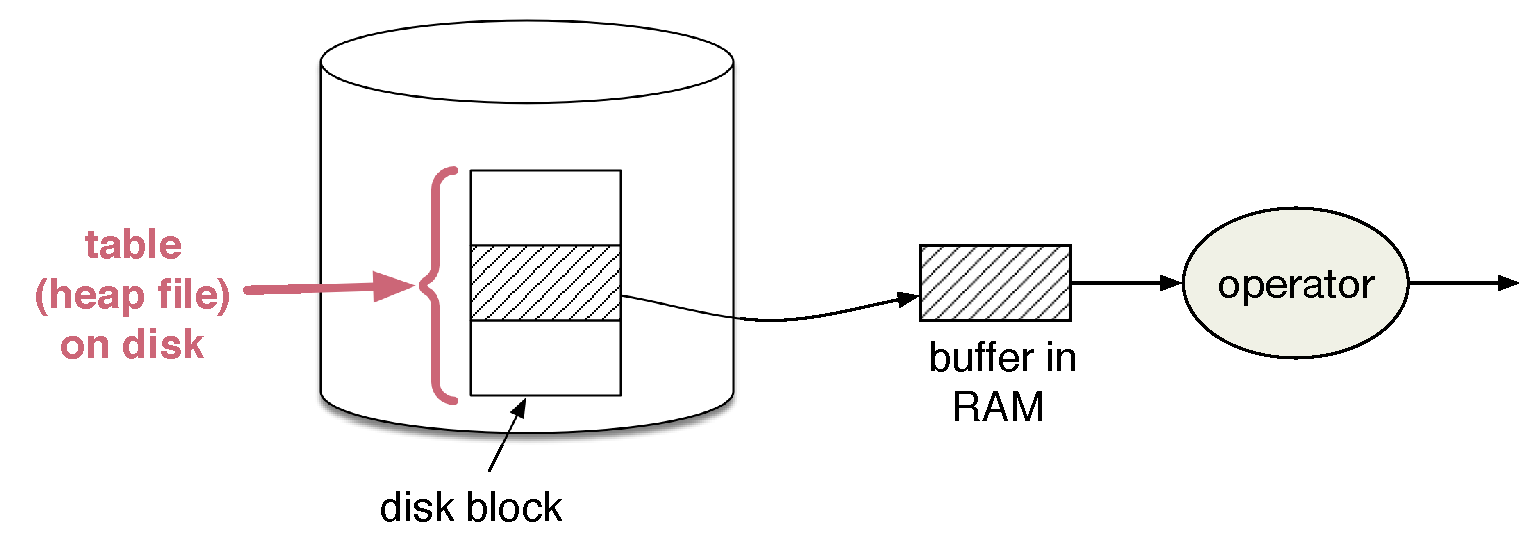
\includegraphics[width=0.75\textwidth]{figures/simple_table_scan}
\end{center}

A table scan requires only one buffer of RAM (which can be reused). But its I/O cost is $O(|R|)$ (as it goes over every disk block).

\end{frame}

%
% ------------------------------------------------
%
\begin{frame}{How do we find the cost of a plan?}

Focus on the iterators that perform I/O or store data in memory.

\vskip2em

\begin{columns}[onlytextwidth]
\begin{column}{0.125\textwidth}
	\begin{tikzpicture}[semithick,align=center,node distance=0.825cm,every node/.style={inner sep=1,outer sep=1,font=\footnotesize}]
	\node (0) at (0,0) {};
	\node (1) [below of=0] {$\pi_{a_1,\ldots,a_n}$};
    \node (2) [below of=1] {$\sigma_C$};
	\node (3) [below of=2] {\lstinline[style=SQL]{scan}($R$)};
    \path[->]
    	(1) edge (0)
        (2) edge (1)
        (3) edge (2);
	\end{tikzpicture}
\end{column}
\begin{column}{0.75\textwidth}
Recall that the iterators for $\sigma$ and $\pi$ do not read any data from disk, thus have 0 I/O cost. \\[1em]

Also, they do not need to keep any data in buffers. So their memory cost is also 0.
\end{column}
\end{columns}

\vskip2em

So the final cost of the plan is
\begin{center}
 \fbox{\alert{$O(1)$ buffers} in RAM} and \fbox{\alert{$O(|R|)$ I/O} operations}
\end{center} 
\end{frame}

%
% ------------------------------------------------
%
\begin{frame}{How many buffers should the DBMS use?}

\vskip1em

A complete table scan \underline{can be done with a single buffer}.

\vskip1em

But... IF there is more RAM available, \alert{should the DBMS read more blocks at once (maybe all of them) OR ... should it save RAM}?

\vskip1em

Reading many consecutive blocks at once is better:\\
 - this amortizes the seek time (for HDDs) and\\
 - reduces the impact of BUS congestion

\end{frame}


%
% ------------------------------------------------
%

\floatstyle{plaintop}
\restylefloat{algorithm}

\newsavebox\nestedLoopJoinAlgorithm
\savebox{\nestedLoopJoinAlgorithm}{
\begin{minipage}{0.7\textwidth}%
\begin{algorithm}[H]
\begin{algorithmic}
% \caption{evaluating $R \Join_C S$}
\ForEach {buffer $b_R$ of $R$}
	\ForEach {buffer $b_S$ of $S$}
		\ForEach {tuple $t_R$ in $b_R$}
			\ForEach {tuple $t_S$ in $b_S$}
				\State $t' \leftarrow \text{join}(t_R,t_S)$ 
				\If {$t'$ satisfies $C$}
					\State \Return $t'$ 
				\EndIf
			\EndFor
		\EndFor
	\EndFor
\EndFor
\end{algorithmic}
\end{algorithm}
\end{minipage}}

\begin{frame}{The I/O cost of joins and products}
\label{nested_loop_join}

To find out \textbf{the actual I/O cost} of the nested-loop-join algorithm of slide~\ref{nested_loop_join_iterator}, consider what happens when we take the calls to \lstinline[style=SQL]{GetNext()} in table scans into account:

\vspace*{-1em}

\begin{columns}
\begin{column}{0.5\textwidth}
\begin{center}
\scalebox{0.75}{\usebox\nestedLoopJoinAlgorithm}
\label{alg:nested_loop_join}
\end{center}
\end{column}

\begin{column}{0.3\textwidth}
\begin{center}
	\begin{tikzpicture}[semithick,align=center,node distance=0.825cm,every node/.style={inner sep=1,outer sep=1,font=\footnotesize}]
	\node (0) at (0,0) {};
    \node (1) [below of=0] {$\Join_C$};
	\node (2) [below of=1,xshift=-1cm] {\lstinline[style=SQL]{scan}($R$)};
	\node (3) [below of=1,xshift=1cm] {\lstinline[style=SQL]{scan}($S$)};

    \path[commutative diagrams/.cd, every arrow, every label]
        (1) edge (0)
        (2) edge (1)
        (3) edge (1);
	\end{tikzpicture}
\end{center}
\end{column}
\end{columns}

So, how many block reads are done?

\end{frame}

%
% ------------------------------------------------
%
\begin{frame}

\vskip1em

\begin{columns}[onlytextwidth]
\begin{column}{0.6\textwidth}
\textbf{Case 1:} use \underline{one} buffer for each scan.
\\[1em]
Memory Cost = 2 buffers\\
I/O Cost = \onslide<2->{\fbox{$O(|R| \cdot |S|)$ block reads}}
\end{column}
\begin{column}{0.45\textwidth}
\scalebox{0.55}{\usebox\nestedLoopJoinAlgorithm}
\end{column}
\end{columns}

\vskip1em

\onslide<2-> \alert{This is the worst case scenario for I/O: quadratic number of block reads.}


\end{frame}


\begin{frame}

\vskip1em

\begin{columns}[onlytextwidth]
\begin{column}{0.6\textwidth}
\textbf{Case 2:} we have $M$ buffers available and $|S| < M-1$.
\end{column}
\begin{column}{0.45\textwidth}
\begin{tikzpicture}
\node at (0,0) [anchor=north west] {\scalebox{0.75}{\alert{load all blocks of $S$ to RAM}}};
\node at (-0.275,0.0125) [anchor=north west]{\scalebox{0.65}{\usebox\nestedLoopJoinAlgorithm}};
\end{tikzpicture}

\end{column}
\end{columns}

\vskip1em

The best case here is to use \underline{one} buffer to scan for $R$, and to \textbf{load all blocks of $S$} to buffers in RAM \alert{beforehand}.

Note that no tuple of either table is read from disk more than once.

\vskip0.5em

\begin{center}
Memory Cost = \onslide<2->{\fbox{$|S|+1$}} and I/O Cost = \onslide<3->{\fbox{$|R|+|S|$}}
\end{center}
\end{frame}

%
% ------------------------------------------------
%
\begin{frame}


\textbf{Case 3:}  $M$ buffers available and $M<|S|\leq|R|$.

Now the best way is to break the inner table into \emph{chunks} of $M-1$ blocks, and make multiple passes on $R$ using a single buffer:

\begin{tikzpicture}
\node at (0,0) {\scalebox{0.75}{\begin{minipage}{1.2\textwidth}%
\begin{algorithm}[H]
\begin{algorithmic}
\ForEach {\alert{chunk of $M-1$ blocks of $S$}}
\ForEach {buffer $b_R$ of $R$}
	\ForEach {tuple $t_R$ in $b_R$}
		\ForEach {buffer $b_S$ of $S$ \alert{in memory}}
			\ForEach {tuple $t_S$ in $b_S$}
				\State $t' \leftarrow \text{\alert{join}}(t_R,t_S)$ 
				\If {$t'$ satisfies $C$}
					\State return $t'$ 
				\EndIf
			\EndFor
		\EndFor
	\EndFor
\EndFor
\EndFor
\end{algorithmic}
\end{algorithm}
\end{minipage}}};

\node at (4.5,-0.25) {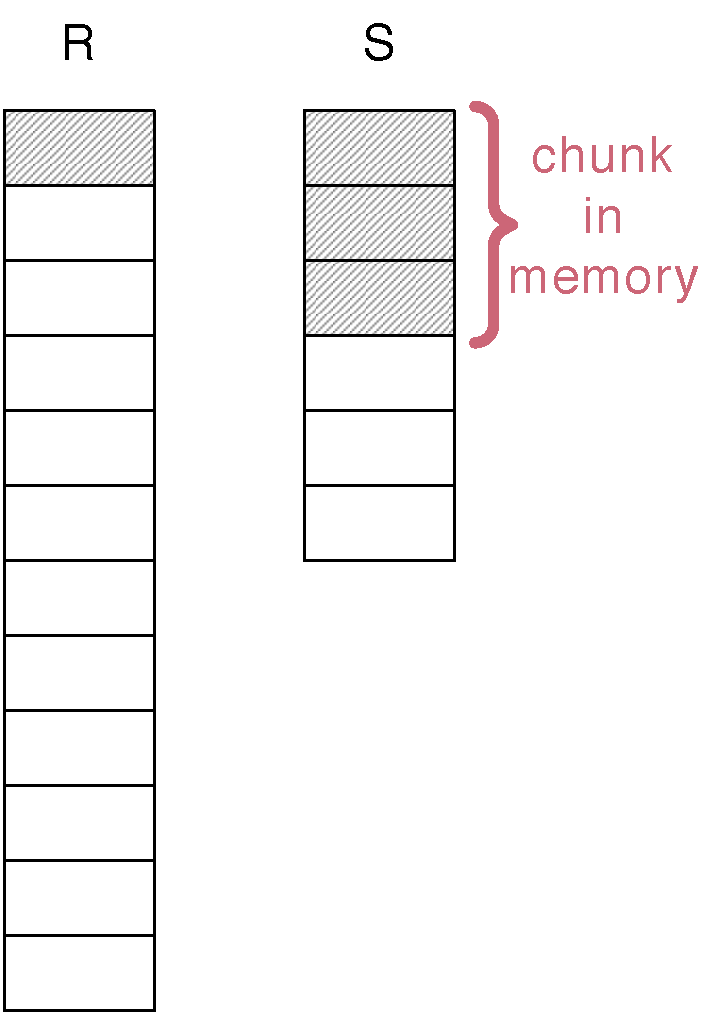
\includegraphics[width=0.3\textwidth]{figures/nested_loop_join.pdf}};

\end{tikzpicture}
\end{frame}

%
% ------------------------------------------------
%
\begin{frame}
\label{example_cost_nested_loop_join}
Cost:

\vskip2em

\begin{columns}[onlytextwidth]
\begin{column}{0.6\textwidth}

I/O: \(\ceil*{\frac{|S|}{M-1}}(|R|) + |S|\) block reads

\vskip1em

Memory: $M$ buffers

\vskip2em

\textbf{Example}:\\
- $|R|$ = 12 disk blocks\\
- $|S|$ = 6 disk blocks\\
- $M=4$ memory buffers available

\vskip2em

$\ceil*{\frac{6}{3}} = 2$ chunks;\\ total cost = $(2\cdot 12)+6 = 30$ block reads.
\end{column}
\begin{column}{0.4\textwidth}
\flushright 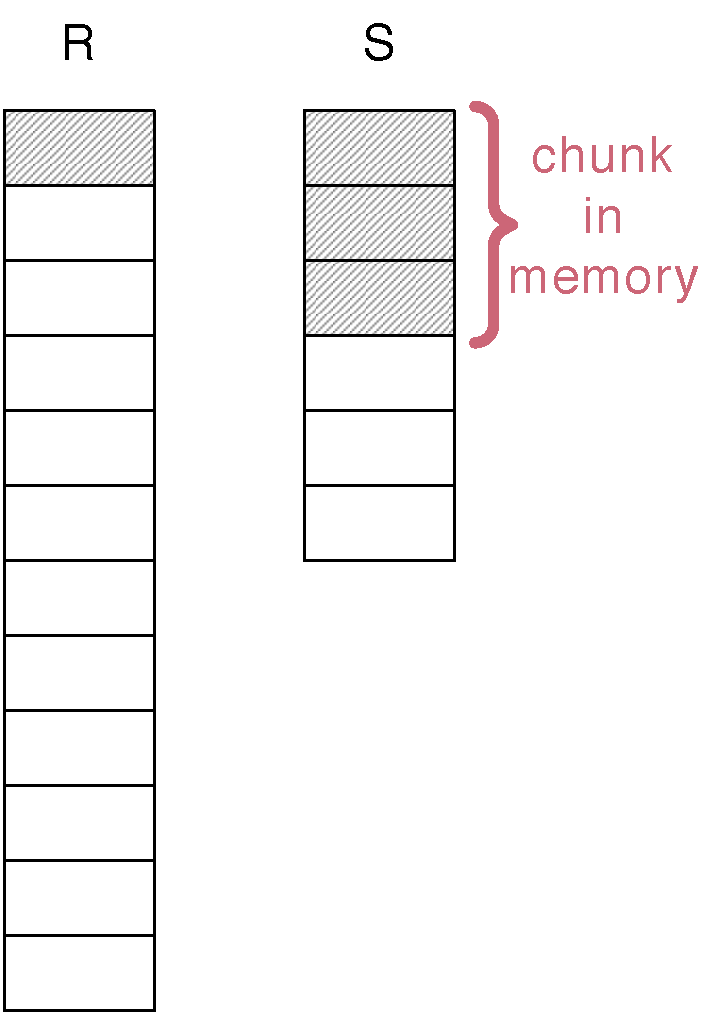
\includegraphics[width=0.75\textwidth]{figures/nested_loop_join.pdf}
\end{column}
\end{columns}
\end{frame}

%
% ------------------------------------------------
%
\begin{frame}{Speeding up the nested loop join}
\label{nested_loop_join_with_indexing_inner_table}

To find matching pairs of tuples faster, the DBMS may \alert{\underline{sort} the tuples of S in memory} (by the join attributes).

If the join is based on an equality (\lstinline[style=SQL]{S.a = R.b}), the DBMS may \alert{build a \underline{hash} table with the tuples of S} (key: \lstinline[style=SQL]{S.a}, value: whole tuple).

\begin{center}
\begin{tikzpicture}[semithick,every node/.style={inner sep=1,outer sep=1,font=\footnotesize}]
\node at (0,0) {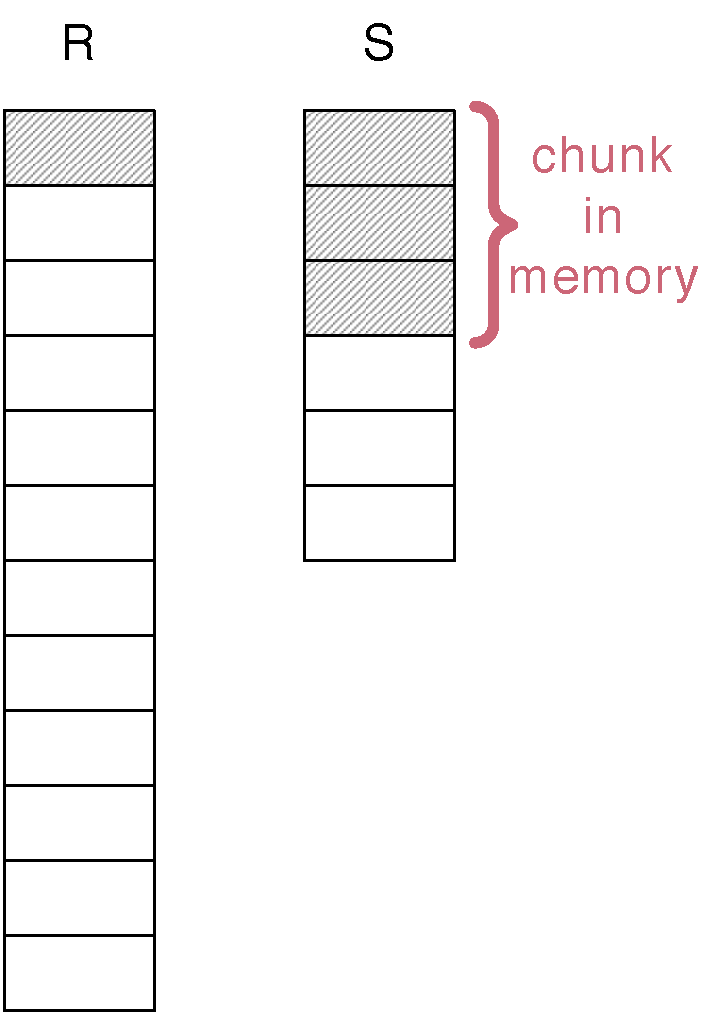
\includegraphics[width=0.3\textwidth]{figures/nested_loop_join.pdf}};

\node (0) at (4,1) [draw,color=accent] {\begin{minipage}{2.15cm}\baselineskip=0.75\baselineskip \centering
sorted/hashed by the join attributes!\end{minipage}};

\draw [->,color=accent] (0) -- (1.75,1.25);
\end{tikzpicture}
\end{center}
\end{frame}

\begin{frame}[fragile]

Example: sorting the results of a sub-expression.

\vskip1em

\begin{columns}[onlytextwidth]
\begin{column}{0.5\textwidth}
\begin{lstlisting}[style=SQL]
SELECT role, imdb
FROM Movie JOIN Cast
WHERE actor='Bill Murray'
\end{lstlisting}
\end{column}
\begin{column}{0.6\textwidth}
\begin{tikzpicture}[semithick,align=center,node distance=0.875cm,every node/.style={inner sep=1,outer sep=1,font=\footnotesize}]
\node (0) at (0,0) {} ; %empty node with ``answer''
\node (1) [below of= 0] {$\pi_{\texttt{role,imdb}}$};
\node (2) [below of= 1] {$\Join$};
\node (3a) [below right of= 2, xshift=1cm] {\lstinline[style=SQL]{sort_by(title,year)}};
\node (3) [below of= 3a] {$\sigma_{\texttt{actor='Bill Murray'}}$};
\node (4) [below left of= 2, xshift=-1cm] {\lstinline[style=SQL]{scan(Movie)}};
\node (5) [below of = 3] {\lstinline[style=SQL]{scan(Cast)}};
\path[->]
    (4) edge (2)
    (5) edge (3) 
    (3) edge (3a)
    (3a) edge (2)
    (2) edge (1)
    (1) edge (0);
\end{tikzpicture}

\end{column}
\end{columns}

\vskip1em

Better yet, we could sort the results of \textbf{both} sub-expressions on the join attributes and perform a sort-based-join (see slide~\ref{sort_based_equality_join_idea}) in memory.

\end{frame}


% \begin{frame}
% \begin{tikzpicture}[semithick,align=center,node distance=0.875cm,every node/.style={inner sep=1,outer sep=1,font=\footnotesize}]
% \node (0) at (0,0) {} ; %empty node with ``answer''
% \node (1) [below of= 0] {$\pi_{\texttt{a,e}}$};
% \node (2) [below of= 1] {$\Join$};
% \node (3) [below right of= 2, xshift=1cm] {\lstinline[style=SQL]{sort_by(a,b)}};
% \node (4) [below left of= 2, xshift=-1cm] {\lstinline[style=SQL]{scan(S)}};
% \node (5) [below of = 3] {\lstinline[style=SQL]{scan(R)}};
% \path[->]
%     (4) edge (2)
%     (5) edge (3) 
%     (3) edge (2)
%     (2) edge (1)
%     (1) edge (0);
% \end{tikzpicture}

% \end{frame}


%
% ------------------------------------------------
%
\begin{frame}{Computing set operations with sorting/hashing}
\label{set_union_one_pass}
\begin{columns}[onlytextwidth]
\begin{column}{0.6\textwidth}

\alert{Set Union $R\cup S$}:

\vskip0.5em

Assumptions:\\
 - $M$ buffers available\\ 
 - $|R| > |S|$ and $|R \cup S| \leq M-1$
\end{column}
\begin{column}{0.4\textwidth}
\flushright\usebox{\genericSetOperator}
\end{column}
\end{columns}

\vskip2em

\begin{enumerate}[label=(\arabic*)]
\item Keep a hash set $H_S$ in memory.

\item Read each block of $S$ using a single buffer $b_S$;
\begin{itemize}[-,topsep=-0.5em]
\item For each $t_S$ in $b_S$: if it is not in $H_S$, add it to $H_S$ and return it to the caller.
\end{itemize}


\item Read each block of $R$ using a single buffer $b_R$;
\begin{itemize}[-,topsep=-0.5em]
\item For each $t$ in $b_R$: if it is not in $H_S$, add it to $H_S$ and return it to the caller.
\end{itemize}

\end{enumerate}
\end{frame}




%
% ------------------------------------------------
%
\begin{frame}
\label{set_intersection_one_pass}
\begin{columns}[onlytextwidth]
\begin{column}{0.6\textwidth}

\alert{Set Intersection $R\cap S$}:

\vskip0.5em

Assumptions:\\
 - $M$ buffers available\\ 
 - $|R| > |S|$ and $|S| \leq M-1$
\end{column}
\begin{column}{0.4\textwidth}
\flushright\usebox{\genericSetOperator}
\end{column}
\end{columns}

\vskip2em

\begin{enumerate}[label=(\arabic*)]
\item Read \underline{all of $S$} into a hash set (size $M-1$ buffers) in memory.

\item Read each block of $R$ to (single) buffer $b_R$;
\begin{itemize}[-,topsep=-0.5em]
\item For each $t$ in $b_R$: if it is in $H_S$, \alert{remove it from $H_S$} and return it to the caller.
\end{itemize}
\end{enumerate}
\end{frame}


%
% ------------------------------------------------
%
\begin{frame}
\label{set_difference_left_one_pass}
\begin{columns}[onlytextwidth]
\begin{column}{0.6\textwidth}

\alert{Set Difference $R - S$ (Algorithm 1)}:

\vskip0.5em

Assumptions:\\
 - $M$ buffers available\\ 
 - \blue{$|R| > |S|$} and $|S \cup (R-S)| \leq M-1$
\end{column}
\begin{column}{0.4\textwidth}
\flushright\usebox{\genericSetOperator}
\end{column}
\end{columns}

\vskip2em

\begin{enumerate}[label=(\arabic*)]
\item Read all of $S$ into a hash set $H_S$ in memory.

\item Read each block of $R$ to (single) buffer $b_R$;
\begin{itemize}[-,topsep=-0.5em]
\item For each $t$ in $b_R$: if it is not in $H_S$, \underline{add it to $H_S$} and return it to the caller.
\end{itemize}
\end{enumerate}
\end{frame}


%
% ------------------------------------------------
%
\begin{frame}
\label{set_difference_right_one_pass}
\begin{columns}[onlytextwidth]
\begin{column}{0.6\textwidth}

\alert{Set Difference $R - S$ (Algorithm 2)}

\vskip0.5em

Assumptions:\\
 - $M$ buffers available\\ 
 - \blue{$|S| > |R|$} and $|R| \leq M-1$
\end{column}
\begin{column}{0.4\textwidth}
\flushright\usebox{\genericSetOperator}
\end{column}
\end{columns}

\vskip2em

\begin{enumerate}[label=(\arabic*)]
\item Read all of $R$ into a hash set $H_R$ in memory.

\item Read each block of $S$ to (single) buffer $b_S$;
\begin{itemize}[-,topsep=-0.5em]
\item For each $t_S$ in $b_S$: if \alert{$t_S$ \textbf{is} in $H_R$} remove it from $H_R$.
\end{itemize}

\item Return the tuples in $H_R$ (one at a time) to the caller.
\end{enumerate}
\end{frame}


%
% ------------------------------------------------
%

\newsavebox{\DISTINCTQUERY}
\begin{lrbox}{\DISTINCTQUERY}
\begin{minipage}{0.5\textwidth}
\begin{lstlisting}[style=SQL,escapeinside={(*}{*)},frame=single]
SELECT DISTINCT (*$a_1$*), ... , (*$a_n$*)
FROM (*$T_1$*) [, (*$T_2$*) [, (*$\ldots$*) [, (*$T_m$*)]]]
WHERE (*$c_1$*) AND (*$c_2$*) AND (*\ldots*) AND (*$c_k$*)
\end{lstlisting}
\end{minipage}
\end{lrbox}

\begin{frame}[fragile]{Duplicate elimination}
\label{duplicate_elimination}

\begin{columns}[onlytextwidth]
\begin{column}{0.7\textwidth}

Removing duplicates is done last in the plan!

\vskip1em

\textbf{Idea}: keep the tuples from the query (\alert{$Q$}) in a hash set, using \underline{up to} $M$ buffers; discard duplicates as they arrive (see slide~\ref{distinct_iterator}).

\vskip1em

\begin{center}
\scalebox{0.75}{\usebox{\DISTINCTQUERY}}
\end{center}


\vskip1em

Assumption: $|\alert{Q}| < M$
\vskip0.5em

Cost = \fbox{0 I/O} and \fbox{$O(|\alert{Q}|)$ buffers.}

\end{column}

\begin{column}{0.3\textwidth}
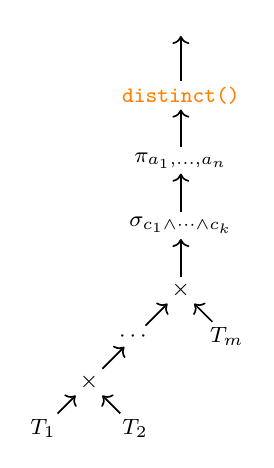
\begin{tikzpicture}[semithick,align=center,node distance=0.825cm,every node/.style={inner sep=1,outer sep=1,font=\footnotesize}]
	\node (0) at (0,0) {};
    \node (1) [below of=0] {\textcolor{orange}{\texttt{distinct()}}};
	\node (2) [below of=1] {$\pi_{a_1,\ldots,a_n}$};
	\node (3) [below of=2] {$\sigma_{c_1 \wedge \cdots \wedge c_k}$};
	\node (4) [below of=3] {$\times$};
	\node (5) [below left of=4] {$\cdots$};
	\node (6) [below right of=4] {$T_m$};
	\node (7) [below left of=5] {$\times$};
	\node (8) [below left of=7] {$T_1$};
	\node (9) [below right of=7] {$T_2$};
    \path[->]
        (1) edge (0)
        (2) edge (1)
        (3) edge (2)
        (4) edge (3)
        (5) edge (4)
        (6) edge (4)
        (7) edge (5)
        (8) edge (7)
        (9) edge (7);
\end{tikzpicture}
\end{column}
\end{columns}
\end{frame}





%%%%%%%%%%%%%%%% ------------------------

\section{Iterators for External Memory}
%!TEX root = lec05_query_processing.tex

%
% --------------------------------------------------------------------------
%
\begin{frame}

If the tables are too large to fit in memory, a good strategy to join them is to create sorted \underline{copies} of the tables on the respective join attributes and scan these tuples in sorted order.

\vskip2em

Example: $R\Join_{R.a=S.b} S$ when $|R|>>|S|>>M$ requires:
\begin{itemize}[-,topsep=-0.5em,noitemsep]
\item Copy of $R$, sorted by \lstinline{R.a}
\item Copy of $S$, sorted by \lstinline{S.b}
\end{itemize}
 
\vskip2em

The DBMS \textbf{must make a copy} of the table, instead of sorting the original table file.
\begin{itemize}[-,topsep=-0.5em]
\item This allows other queries (and even updates) on that table to be executed while the sorting goes on.
\end{itemize}

\end{frame}

%
% --------------------------------------------------------------------------
%
\begin{frame}{Multi-way Merge Sort on external memory:}

\label{multiway_mergesort}

Assume there are $M$ buffers available and you need to sort a file with $|R|>>M$ blocks.

Let $N = \ceil*{\frac{|R|}{M-1}}$.

\vskip1em

\begin{enumerate}[(1)]

\item Load ``chunks'' of $R$ into $M-1$ buffers in memory, sort the tuples, and write the buffers, one buffer at a time, to disk.

\item Merge the $N$ sorted chunks (assuming $N \leq M-1$):
\begin{enumerate}[(a)]
\item Write the output to 1 buffer in memory; flush it to disk when full
\item Read the $N$ sorted chunks using 1 buffer per file
\item Compare the ``current'' tuples in each buffer; add the ``smallest'' to the output buffer; advance that pointer
\end{enumerate}
\end{enumerate}
\end{frame}



%
% --------------------------------------------------------------------------
%
\begin{frame}

\textbf{Step 1:} Sort $N$ individual ``chunks'' of the table in memory, and write them back to disk.

\vskip2em

\begin{center}
\begin{tikzpicture}
\onslide<1|handout:0>{\node at (0,0) {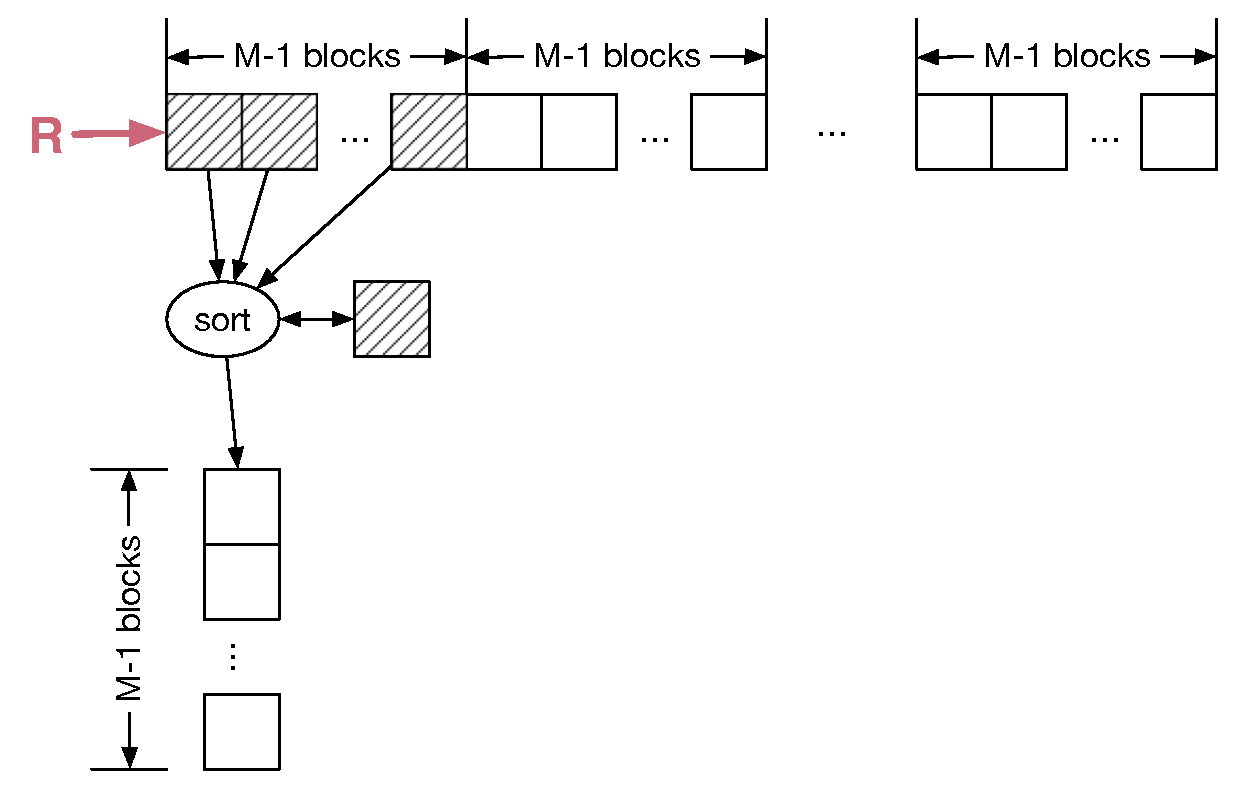
\includegraphics[width=0.75\textwidth]{figures/mergesort/step1.eps}};}
\onslide<2|handout:0>{\node at (0,0) {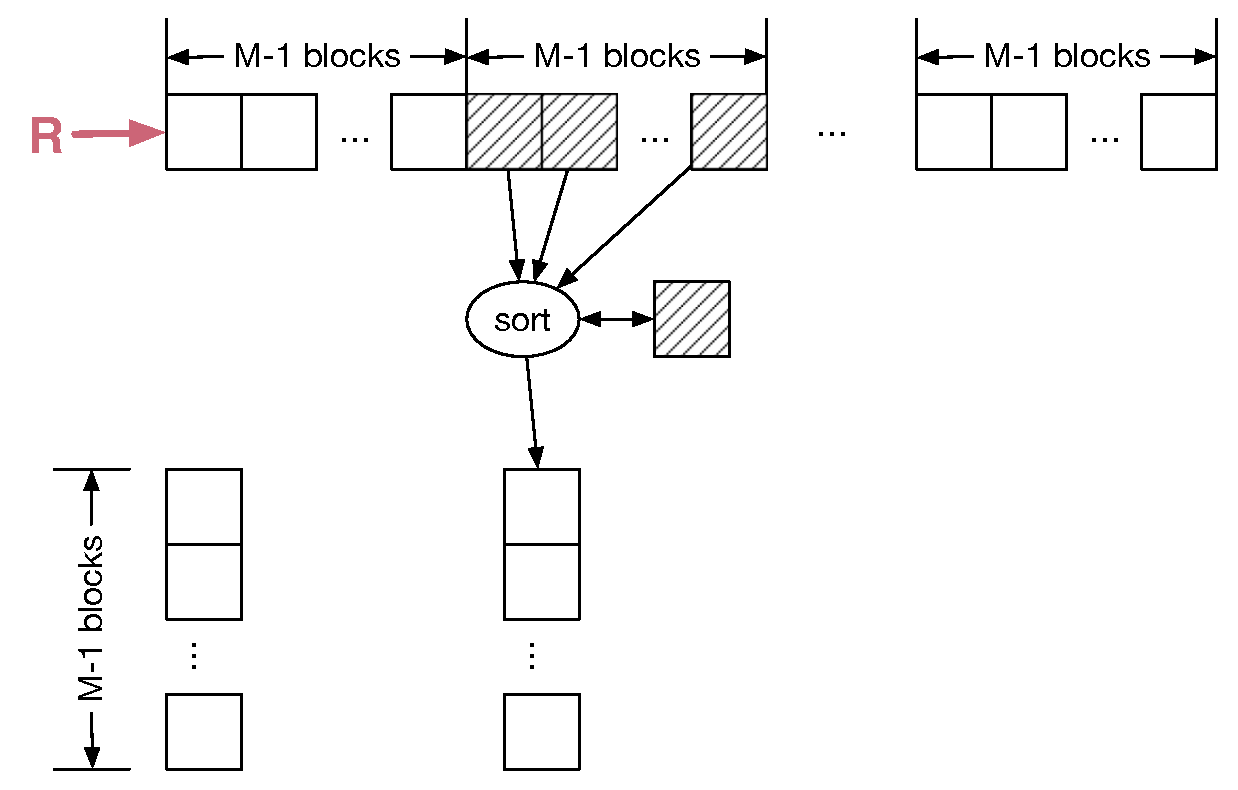
\includegraphics[width=0.75\textwidth]{figures/mergesort/step2.eps}};}
\onslide<3|handout:1>{\node at (0,0) {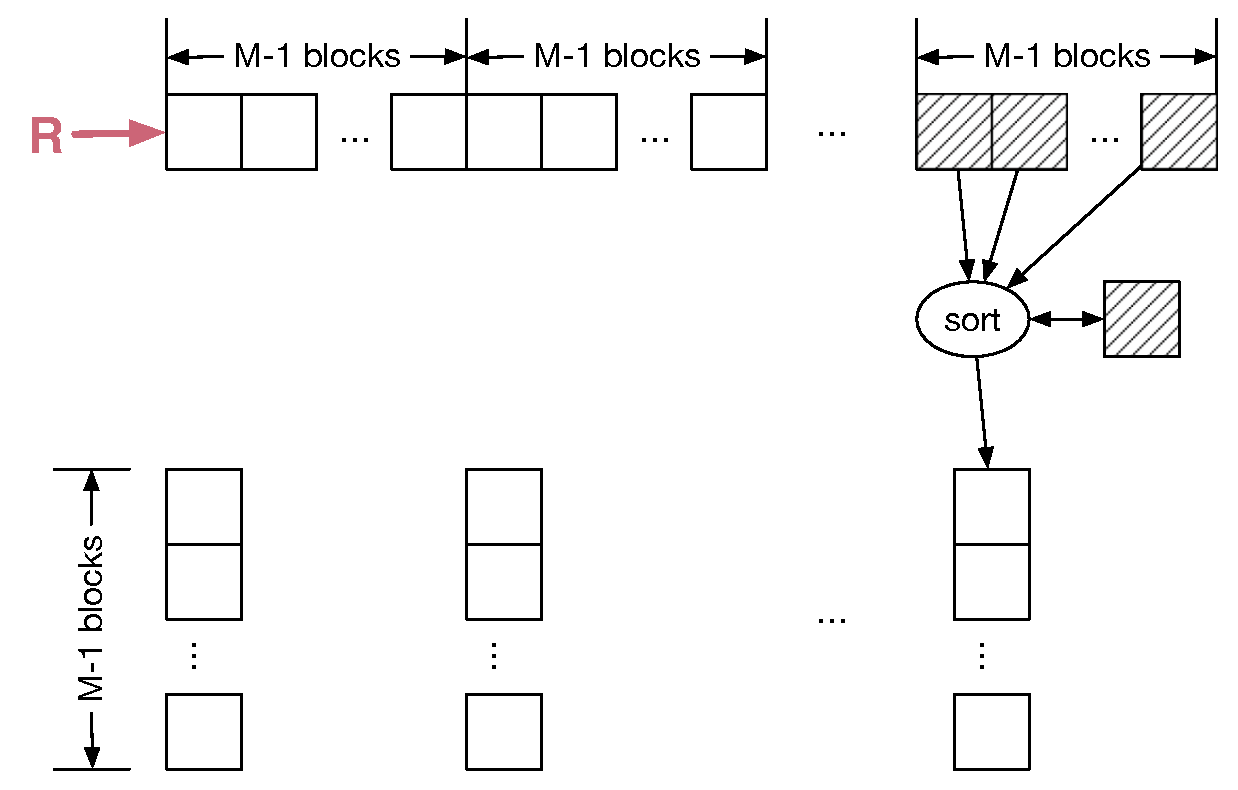
\includegraphics[width=0.75\textwidth]{figures/mergesort/step3.eps}};}
\end{tikzpicture}

\end{center}

\end{frame}

%
% --------------------------------------------------------------------------
%
\begin{frame}

\textbf{Step 2:} Merge the $N$ sorted chunks into a single sorted file. \alert{Case when $N\leq M-1$}:

\vskip2em

\begin{center}
\begin{tikzpicture}
\onslide<1|handout:0>{\node at (0,0) {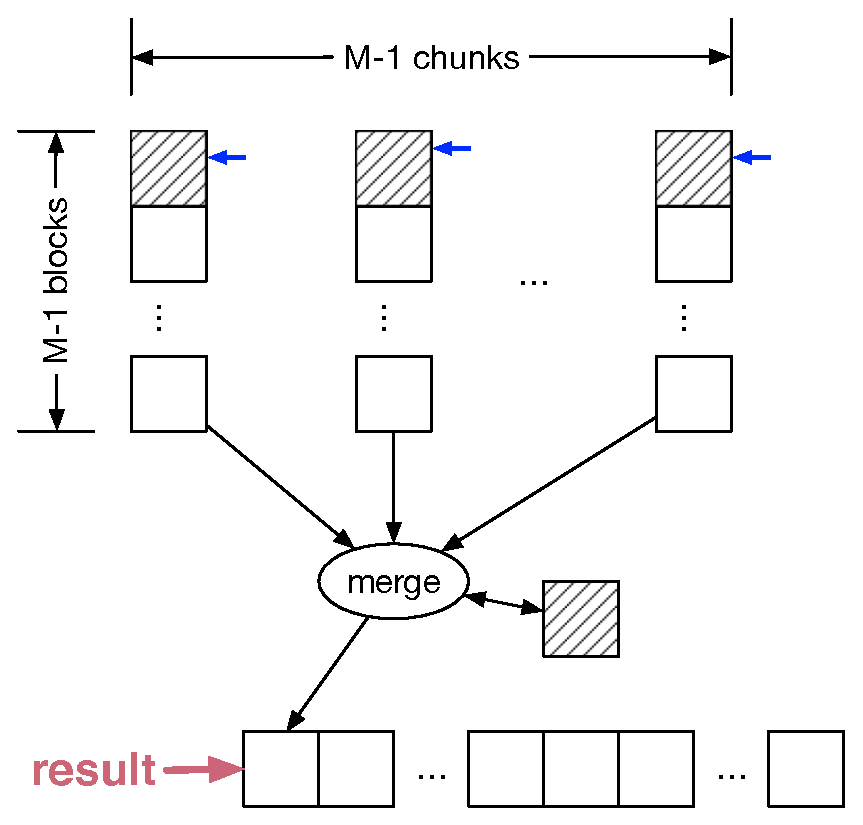
\includegraphics[width=0.5\textwidth]{figures/mergesort/step4.eps}};}
\onslide<2|handout:0>{\node at (0,0) {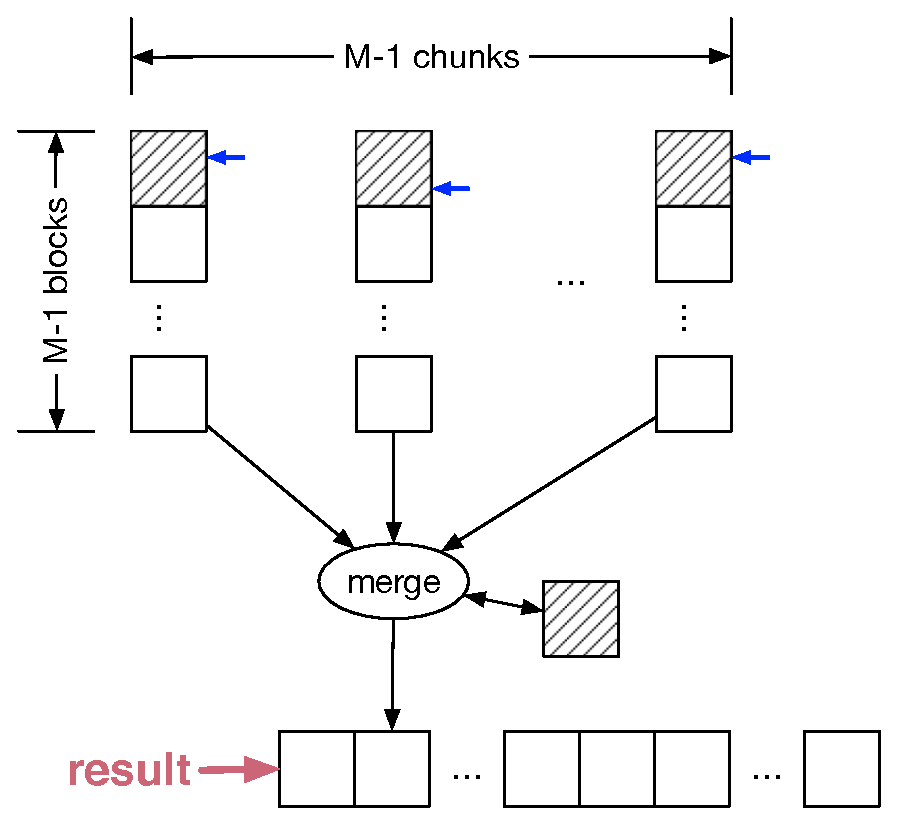
\includegraphics[width=0.5\textwidth]{figures/mergesort/step5.eps}};}
\onslide<3-|handout:1>{\node at (0,0) {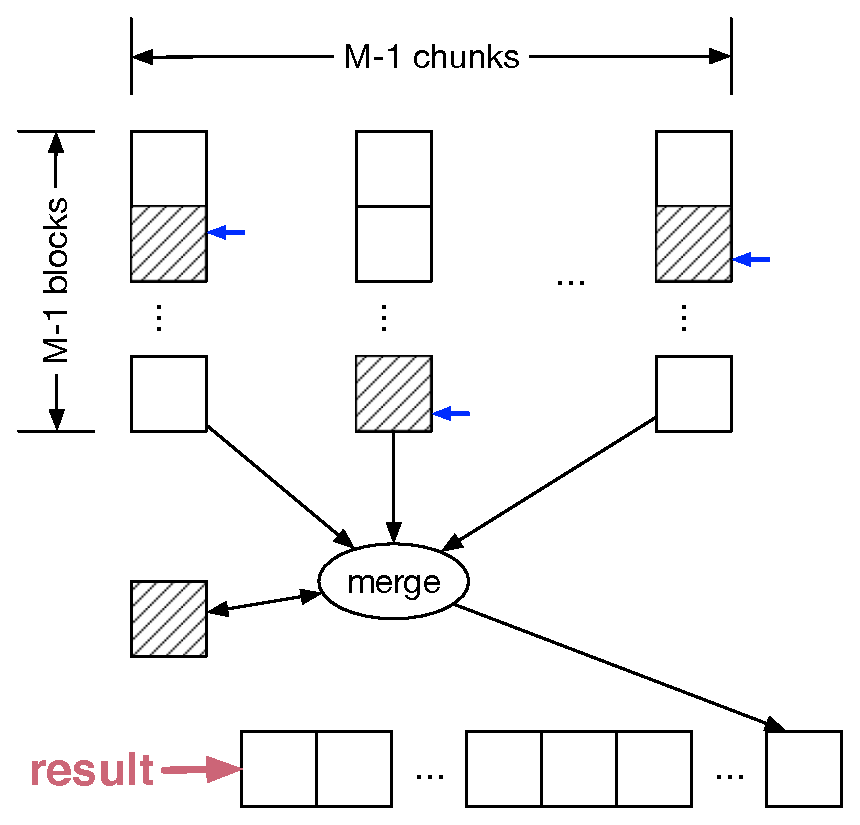
\includegraphics[width=0.5\textwidth]{figures/mergesort/step6.eps}};}
\end{tikzpicture}
\end{center}

\vskip1em

\onslide<4|handout:1>{When $N\leq M-1$ only one merge operation is needed.}

\end{frame}


%
% --------------------------------------------------------------------------
%
\begin{frame}

\textbf{Step 2 revisited} \alert{when $N > M-1$}:

\begin{center}
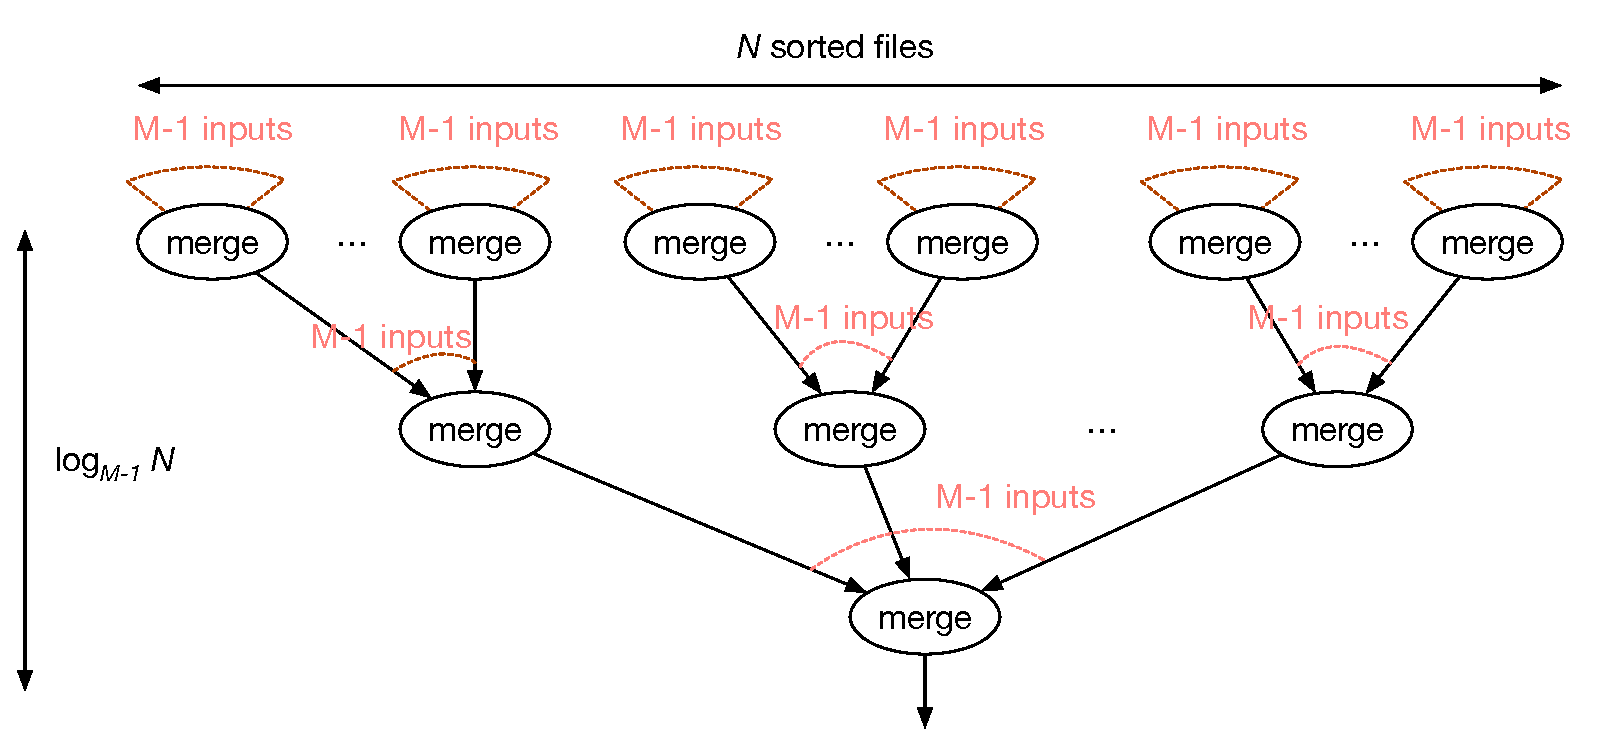
\includegraphics[width=0.85\textwidth]{figures/mergesort/merge_sort_part2_FULL}
\end{center}

This is like in-RAM mergesort, except that each merge steps has $M-1$ inputs \textbf{instead of} two.
\begin{itemize}[-,noitemsep,topsep=-0.5em]
\item The tree has $\ceil*{\log_{M-1}N}$ levels.
\item The entire table is read and written in each level, for a total I/O cost of \fbox{$O(|R|\ceil*{\log_{M-1}N})$}
\end{itemize}
\end{frame}

\begin{frame}

\vskip1em

\textbf{External multi-way mergesort}:\\
$M:$ buffers available; $|R|$: blocks to sort; $N=\ceil*{\frac{|R|}{M-1}}$: chunks.

\begin{itemize}[-]
\item \textbf{Sort phase:} load, sort and write each chunk.
\item \textbf{Merge phase:} start with $\mathit{pass} = 1$
\begin{enumerate}[(1)]
\item Merge the sorted chunks, $M-1$ at a time.
\item If the pass produced $2$ or more chunks, increment $\mathit{pass}$ and repeat step (1).
\end{enumerate}
\end{itemize}

\vskip1em

\begin{block}{How much I/O in total? }

In \blue{each pass} on the file we \alert{read and write} the same amount of data (i.e., the size of the file itself):
\begin{itemize}[-,noitemsep,topsep=-0.5em]
\item Sort phase: $2\cdot |R|$
\item Merge phase: $2 \cdot \ceil*{\log_{M-1}N}|R|$
\end{itemize}

\end{block}
\end{frame}

%
% --------------------------------------------------------------------------
%
\begin{frame}[fragile]

\textbf{Example:} sorting relation \lstinline[style=SQL]{Member(name, class)} on \lstinline[style=SQL]!class! with $M=3$.

\vskip2em

\begin{center}
\begin{tikzpicture}
\onslide<1|handout:0>{\node at (0,0) {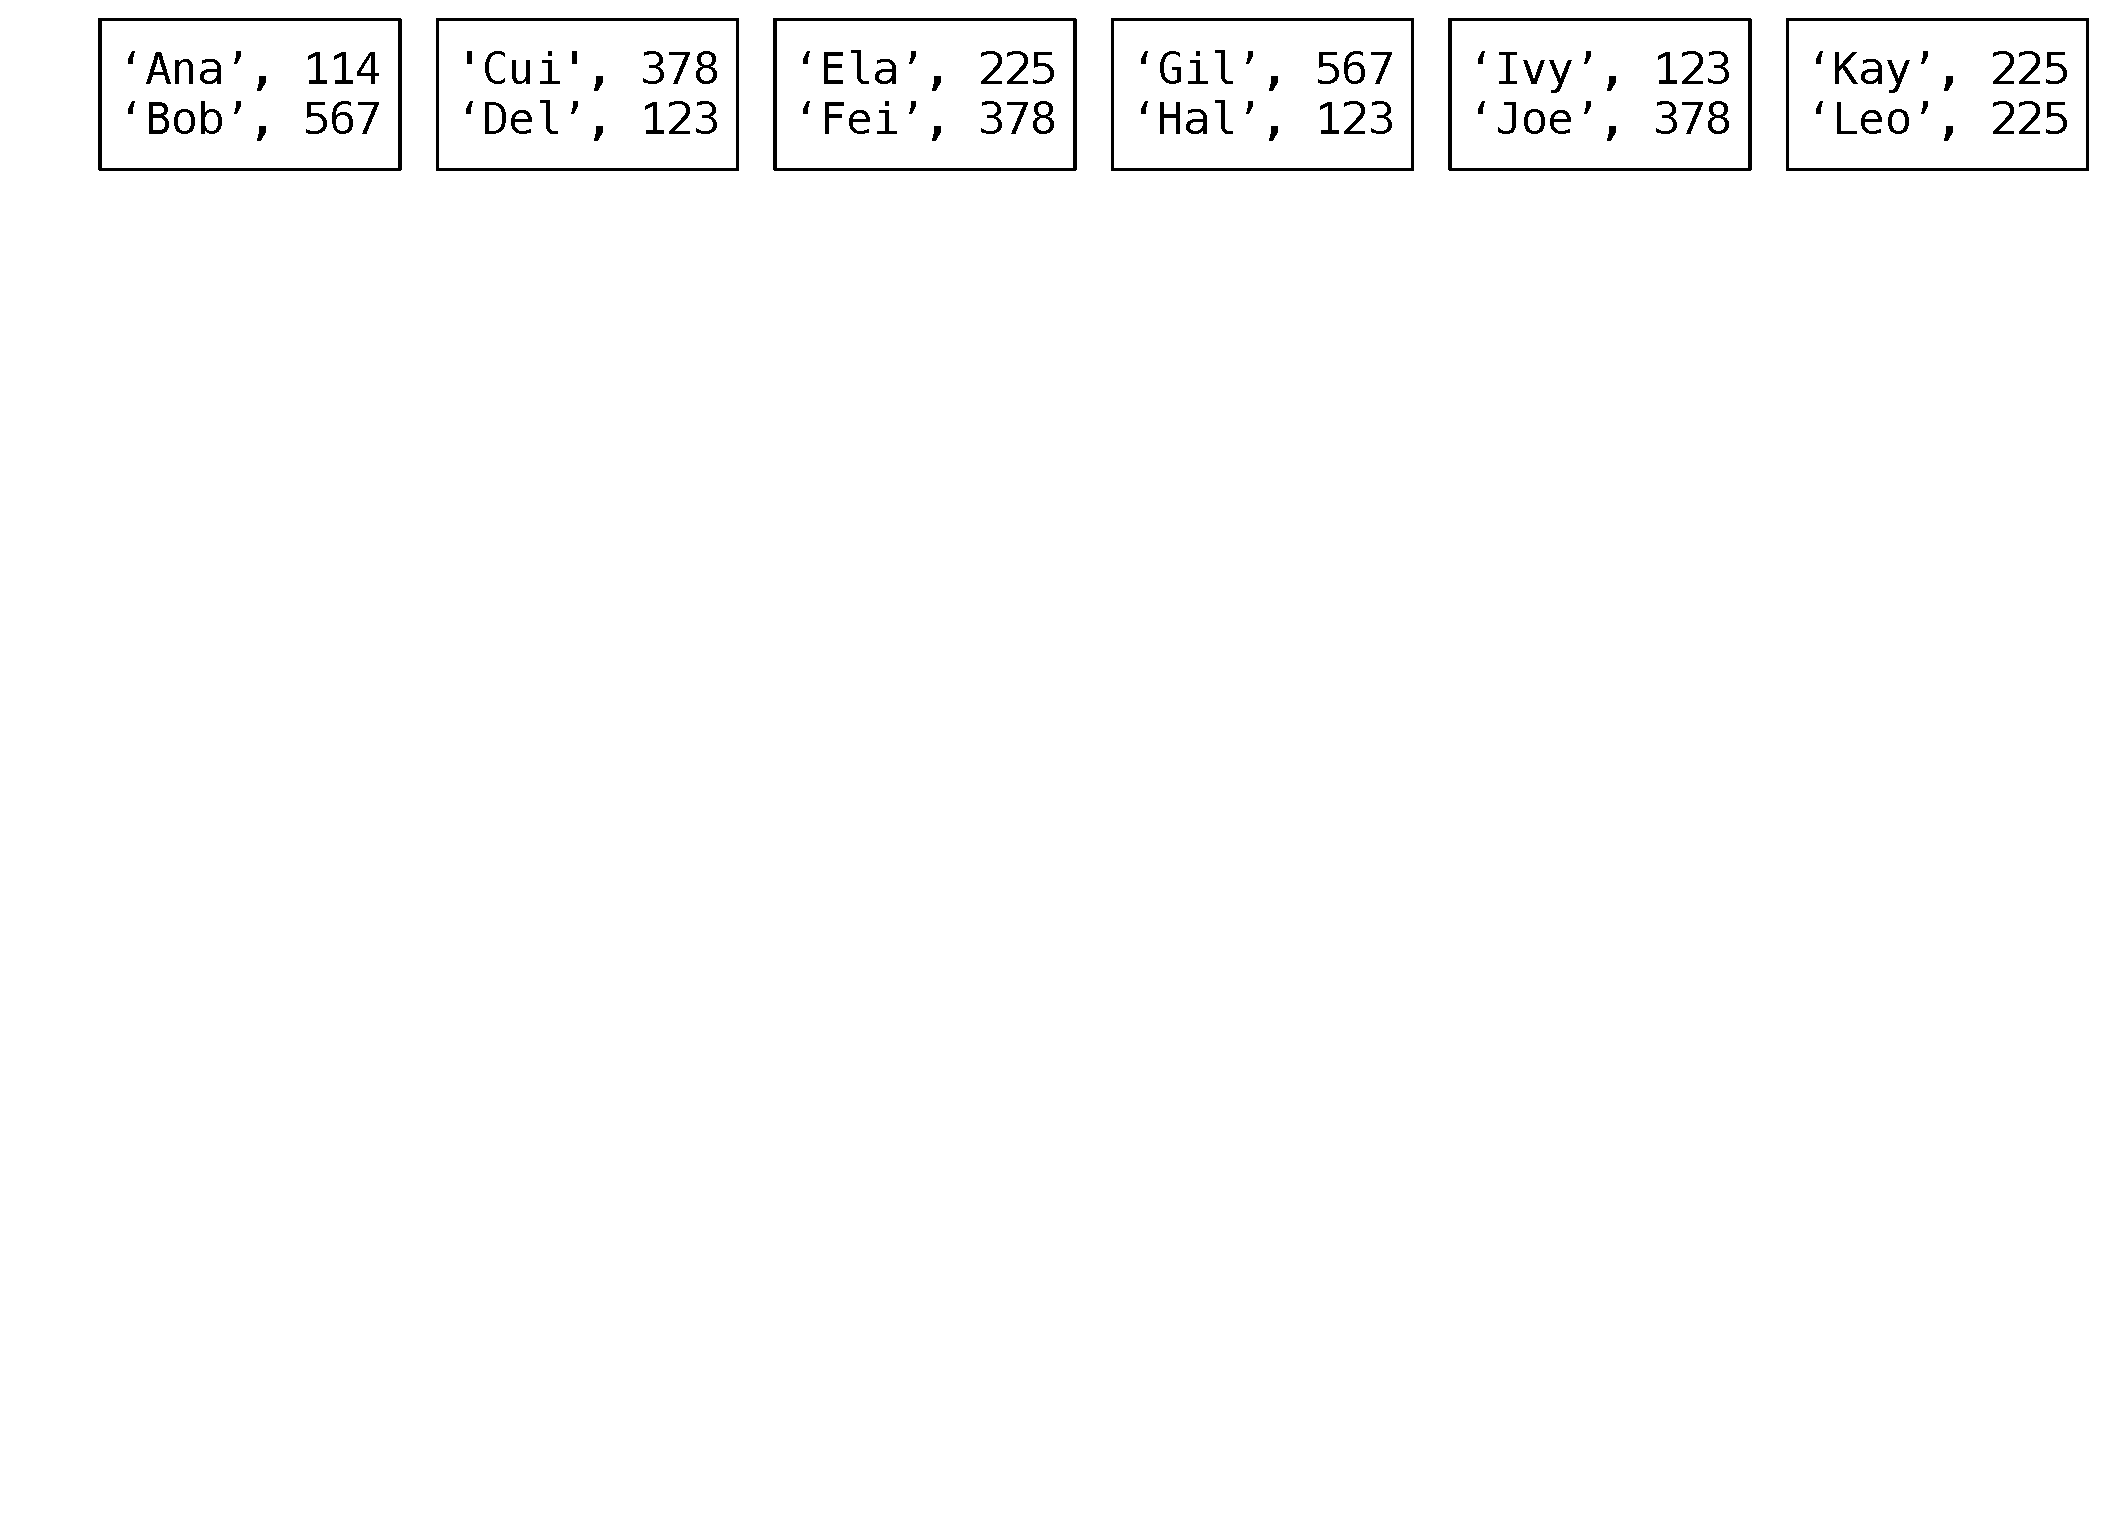
\includegraphics[width=0.9\textwidth]{figures/mergesort_example/step1.eps}};}
\onslide<2|handout:0>{\node at (0,0) {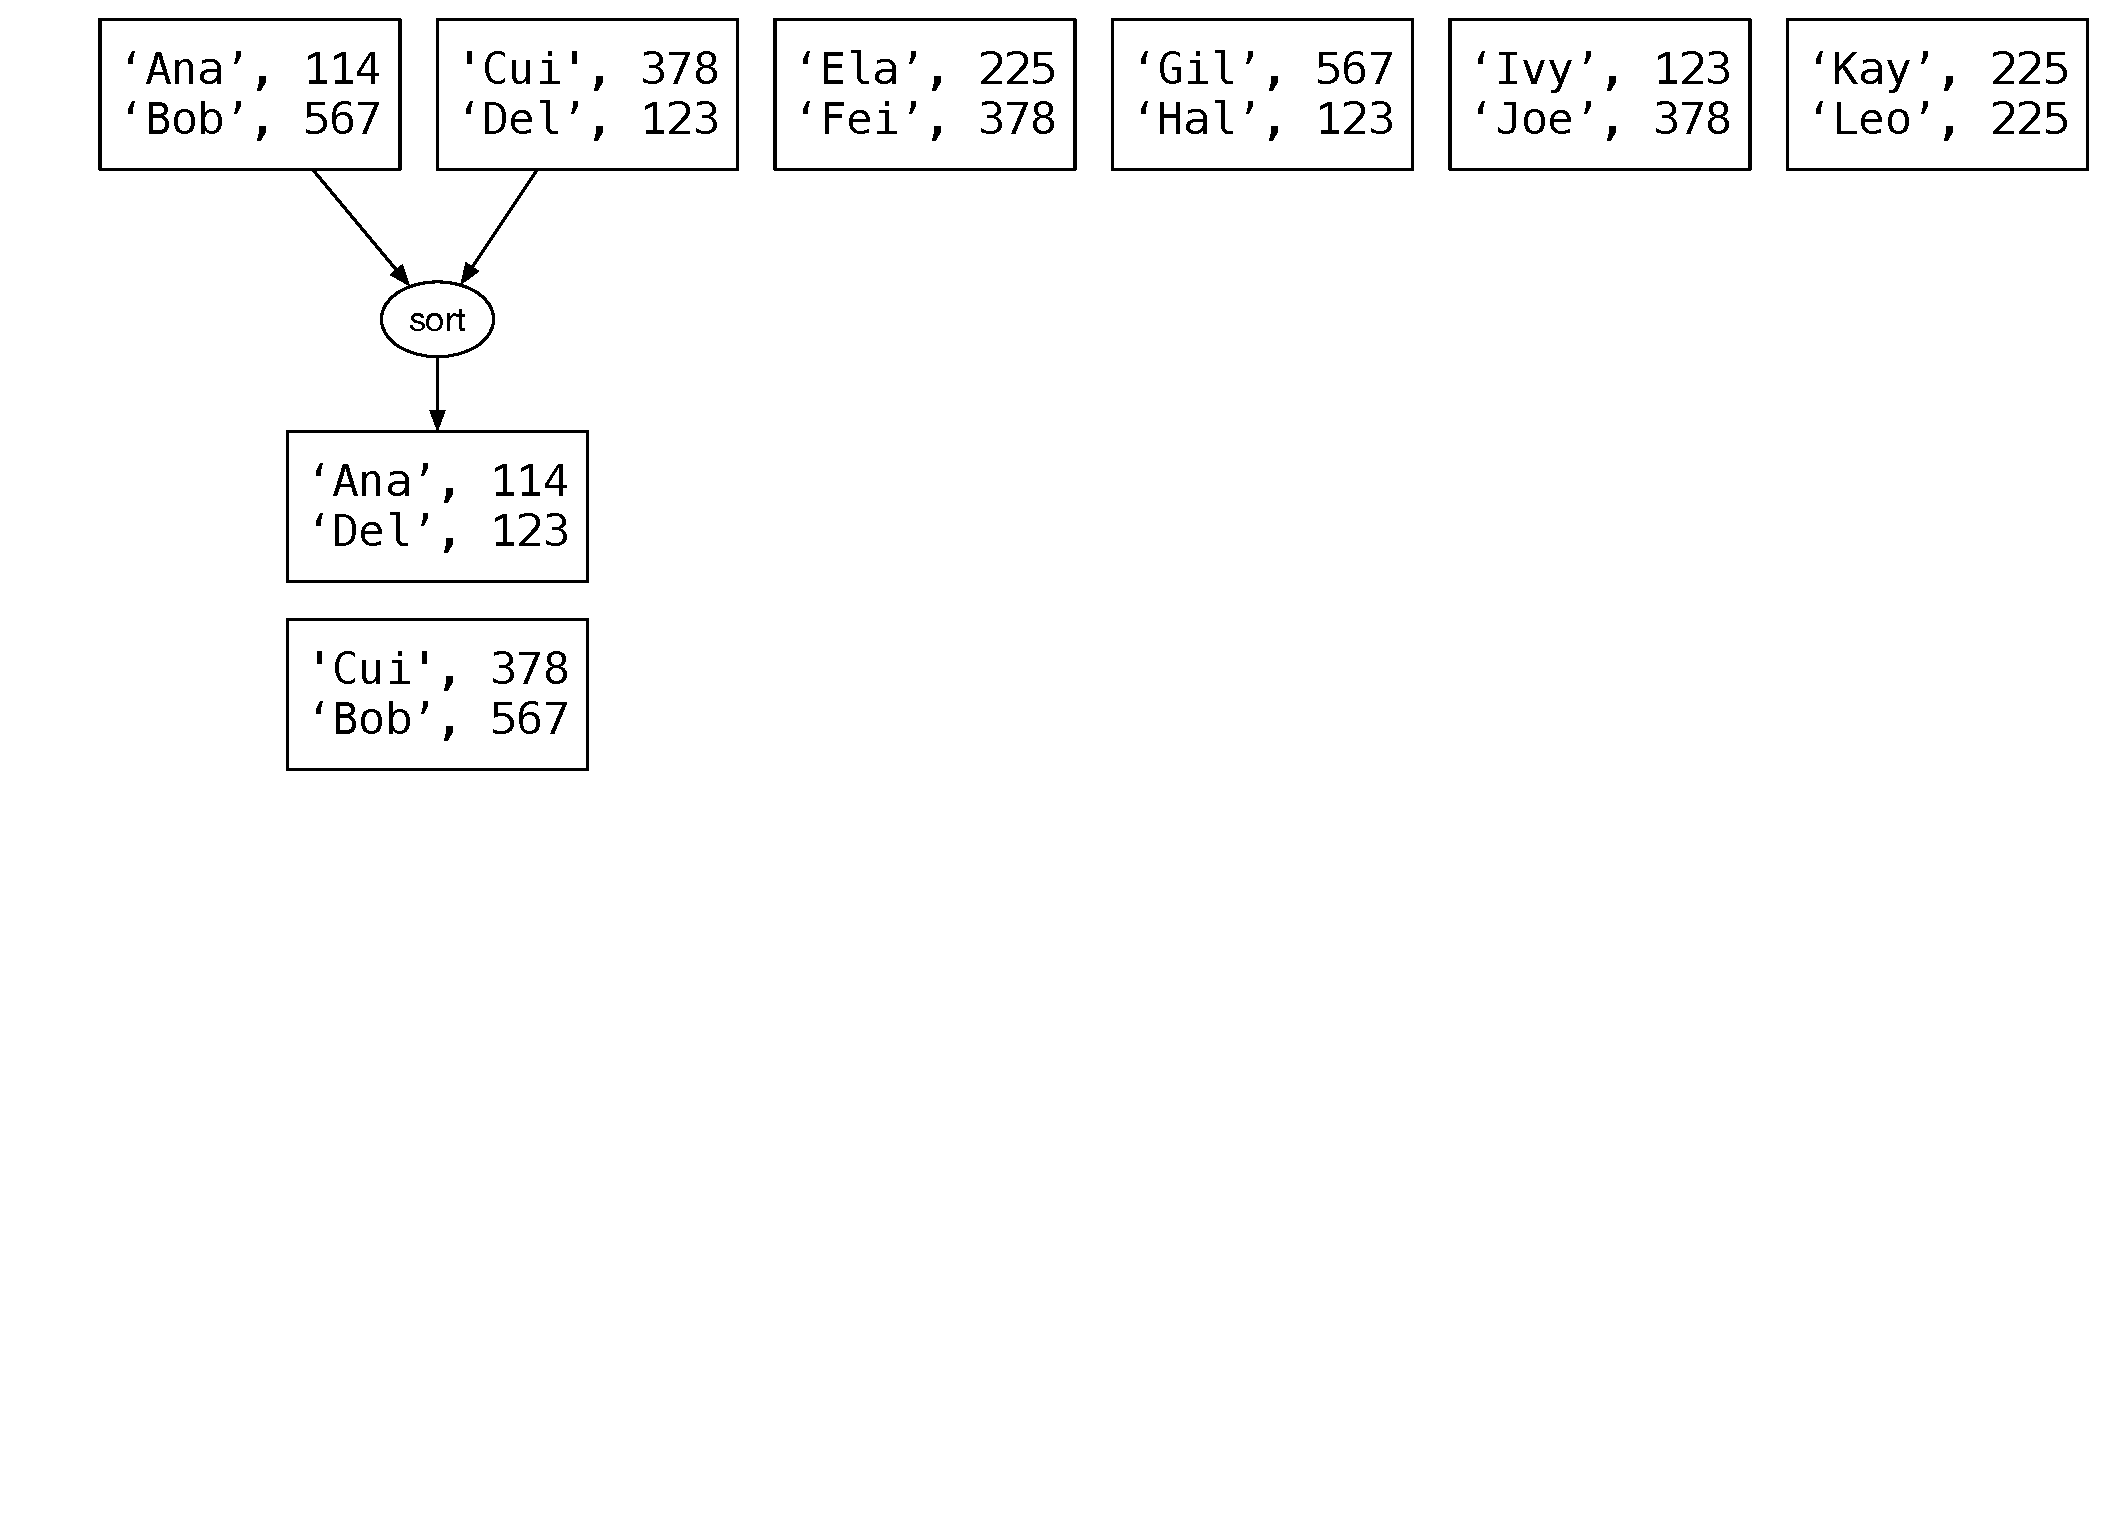
\includegraphics[width=0.9\textwidth]{figures/mergesort_example/step2.eps}};}
\onslide<3|handout:0>{\node at (0,0) {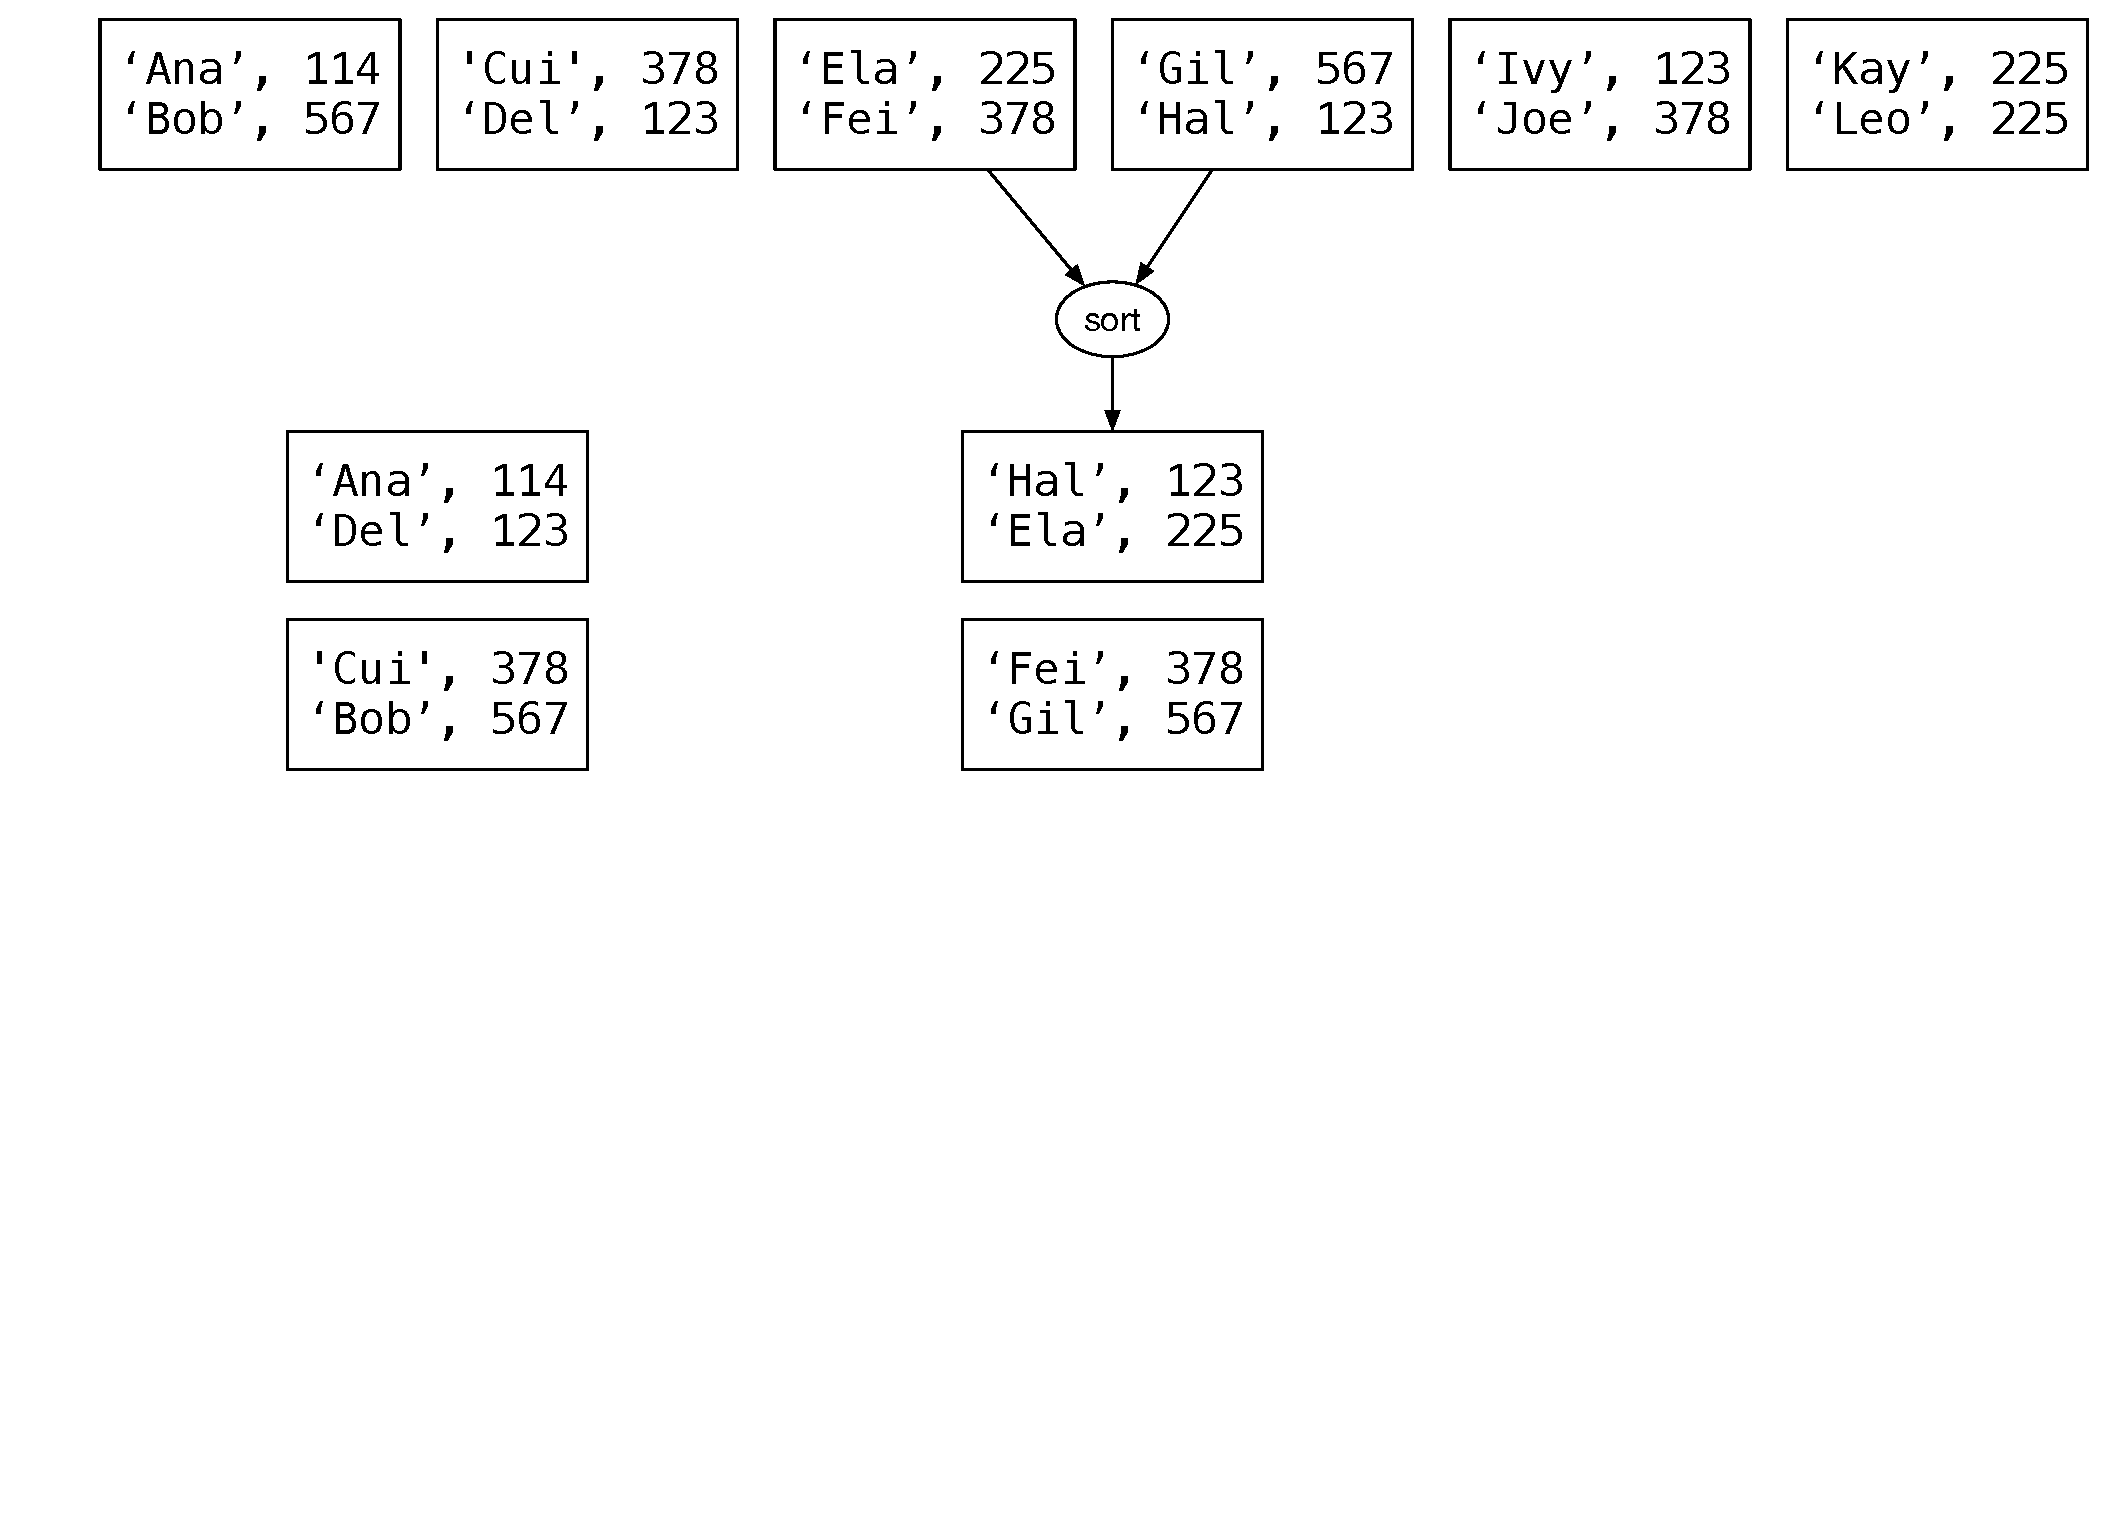
\includegraphics[width=0.9\textwidth]{figures/mergesort_example/step3.eps}};}
\onslide<4|handout:0>{\node at (0,0) {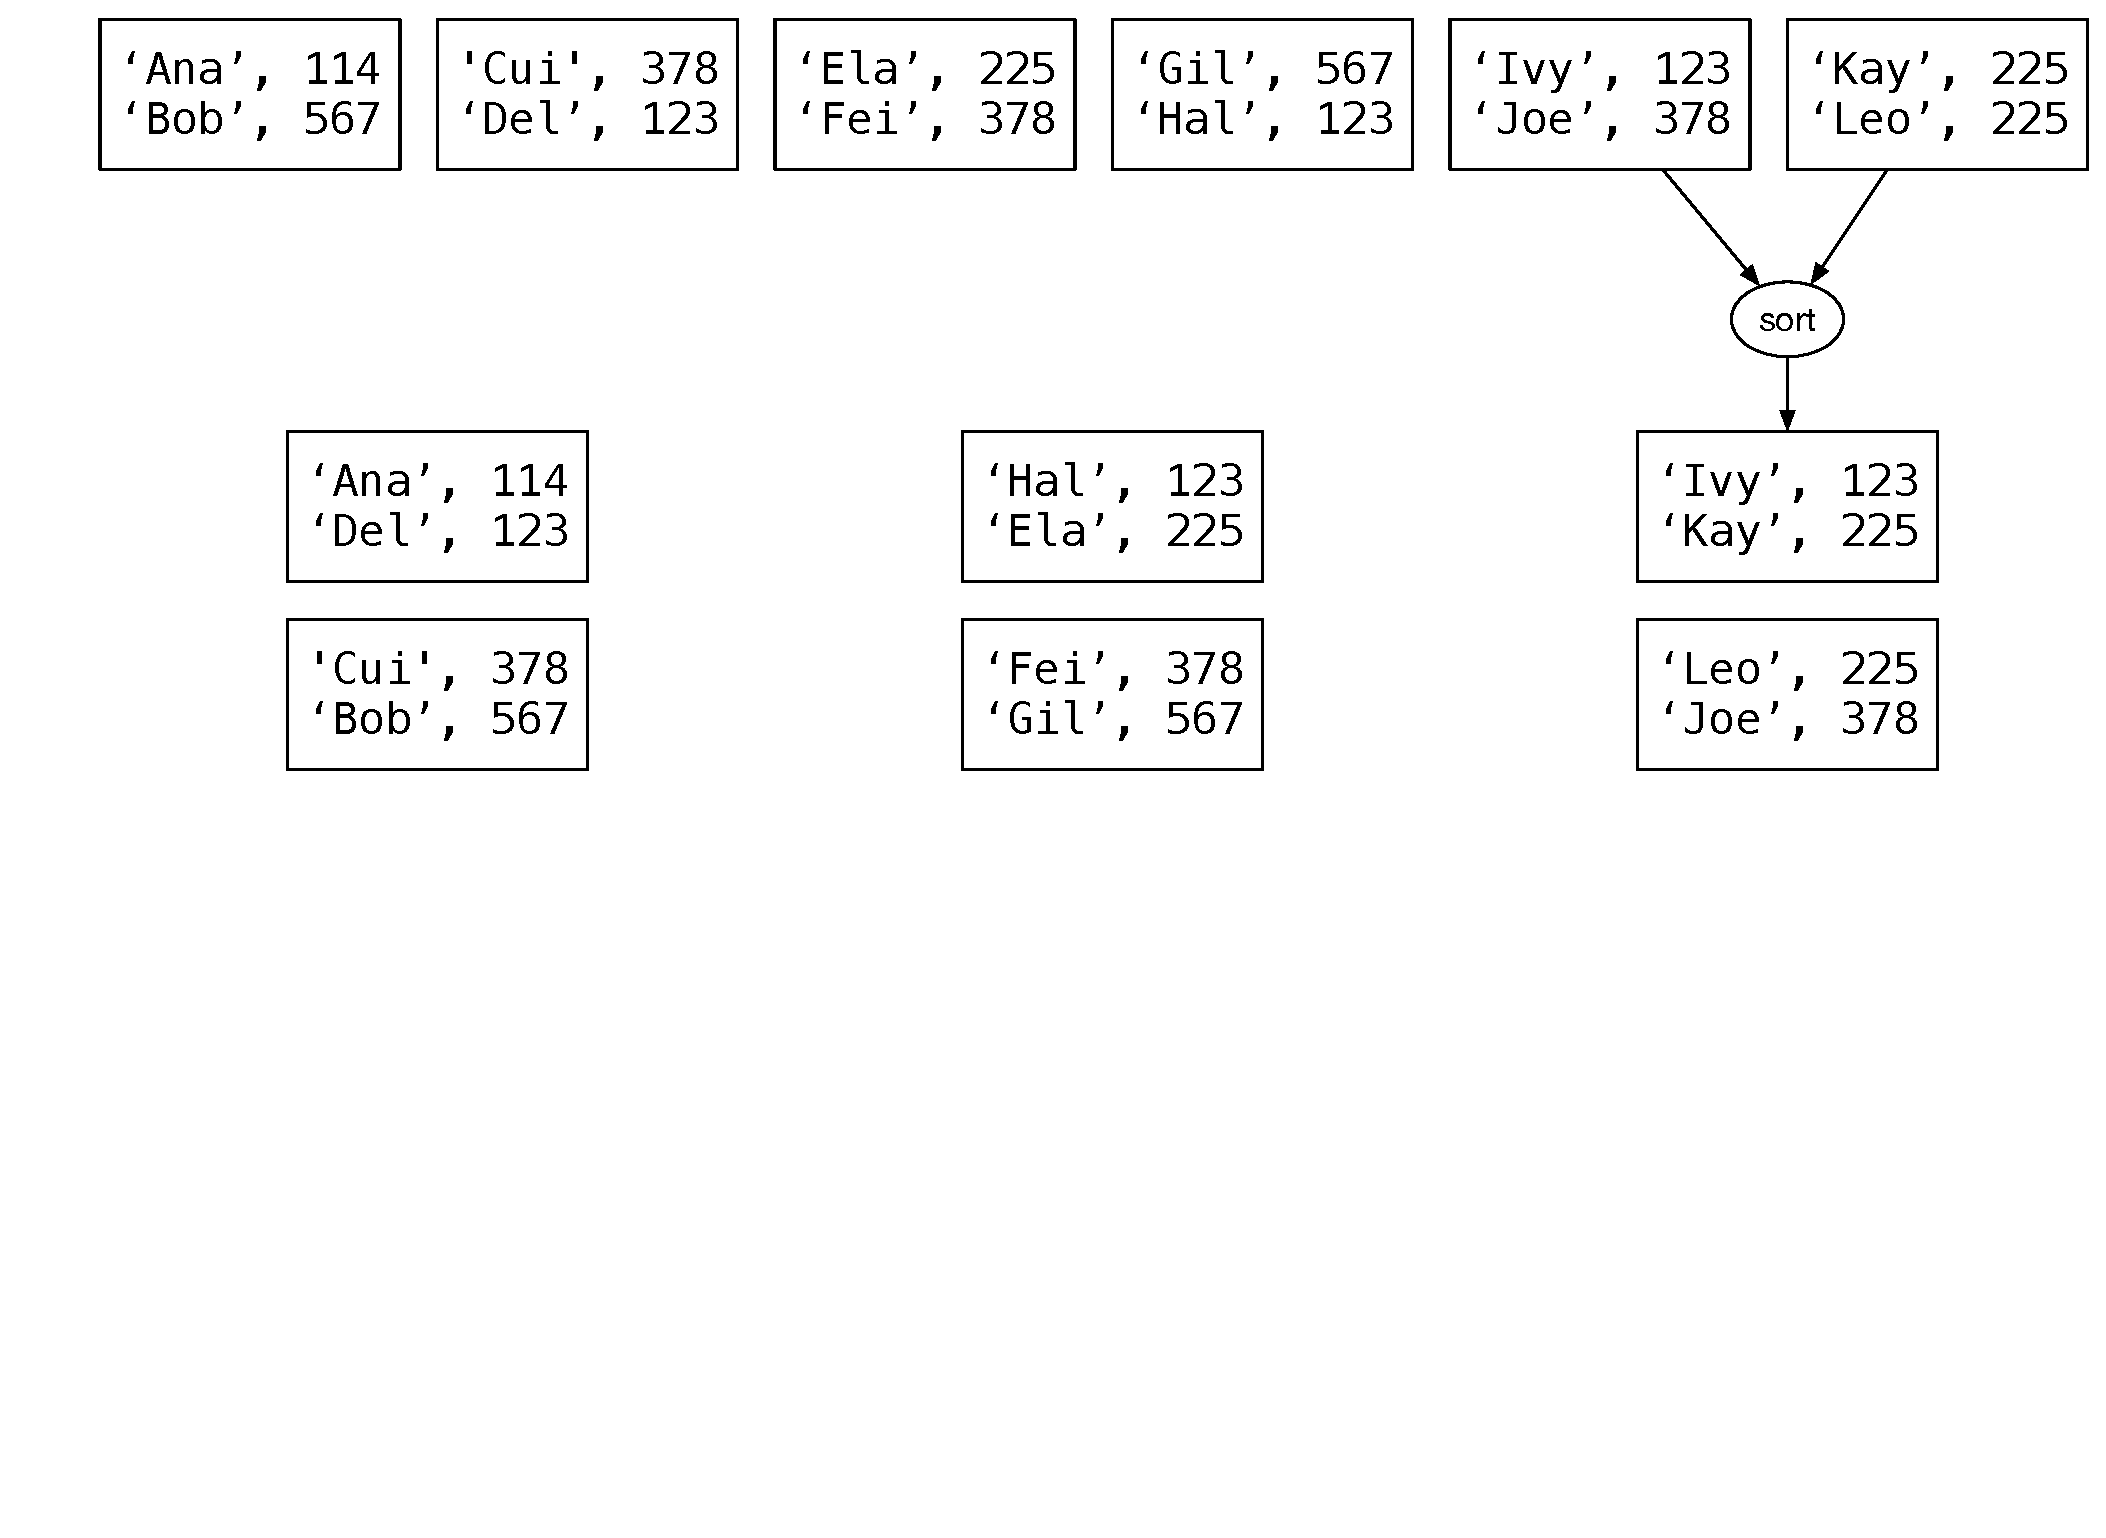
\includegraphics[width=0.9\textwidth]{figures/mergesort_example/step4.eps}};}
\onslide<5|handout:0>{\node at (0,0) {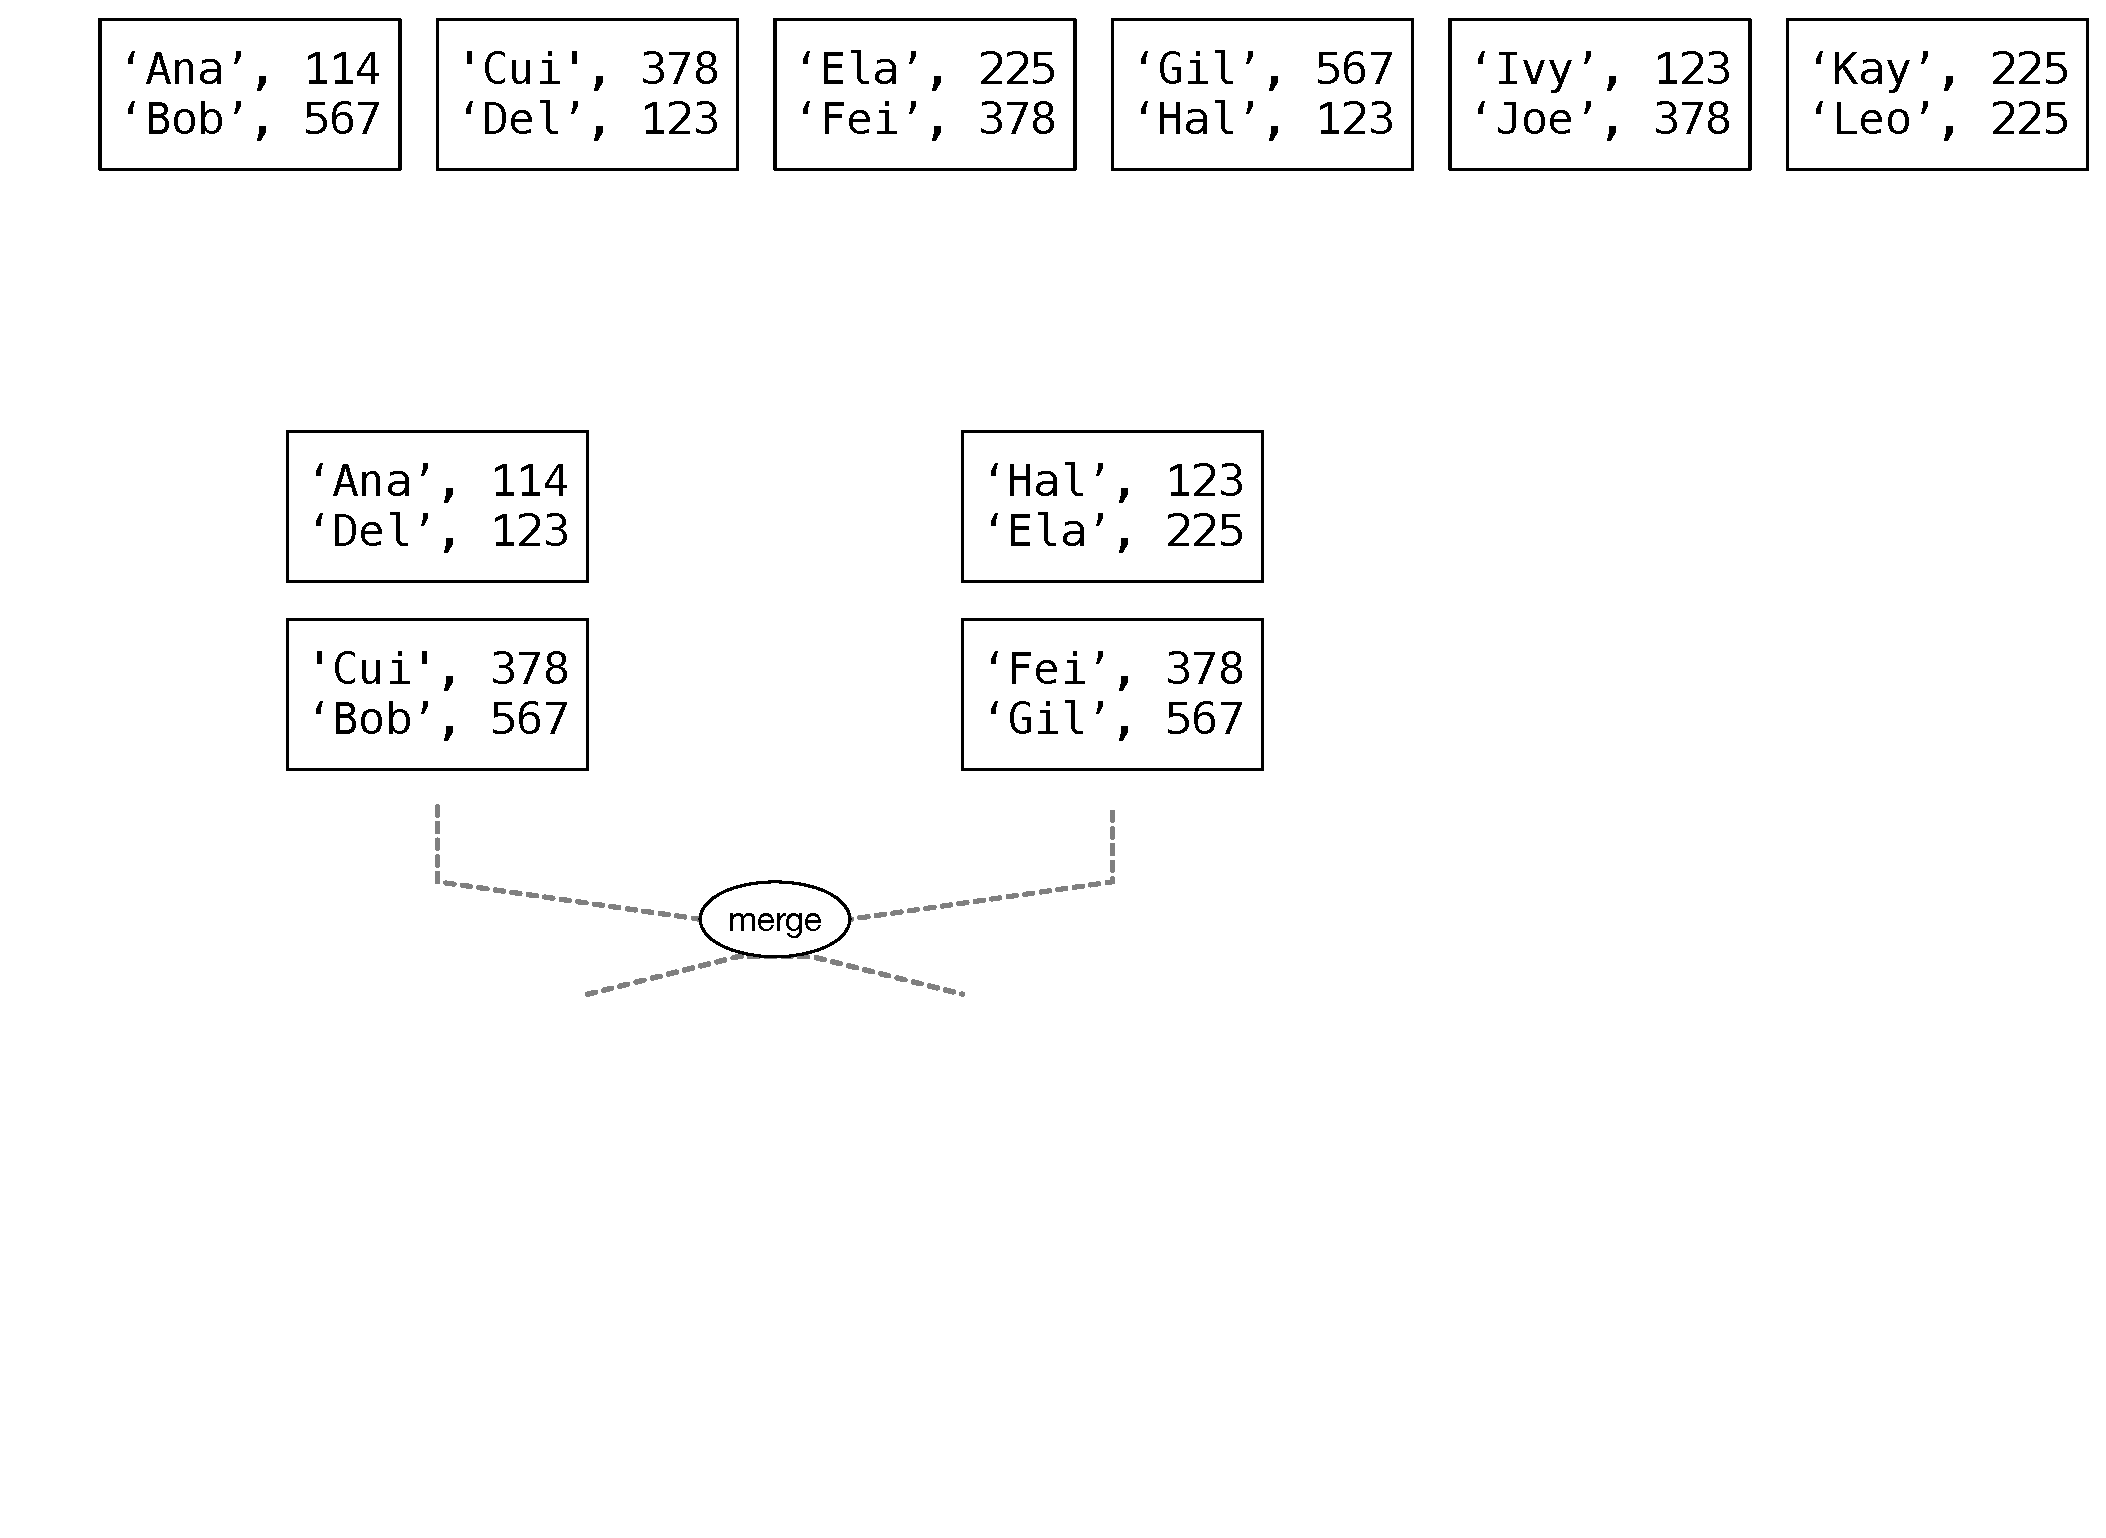
\includegraphics[width=0.9\textwidth]{figures/mergesort_example/step5.eps}};}
\onslide<6|handout:0>{\node at (0,0) {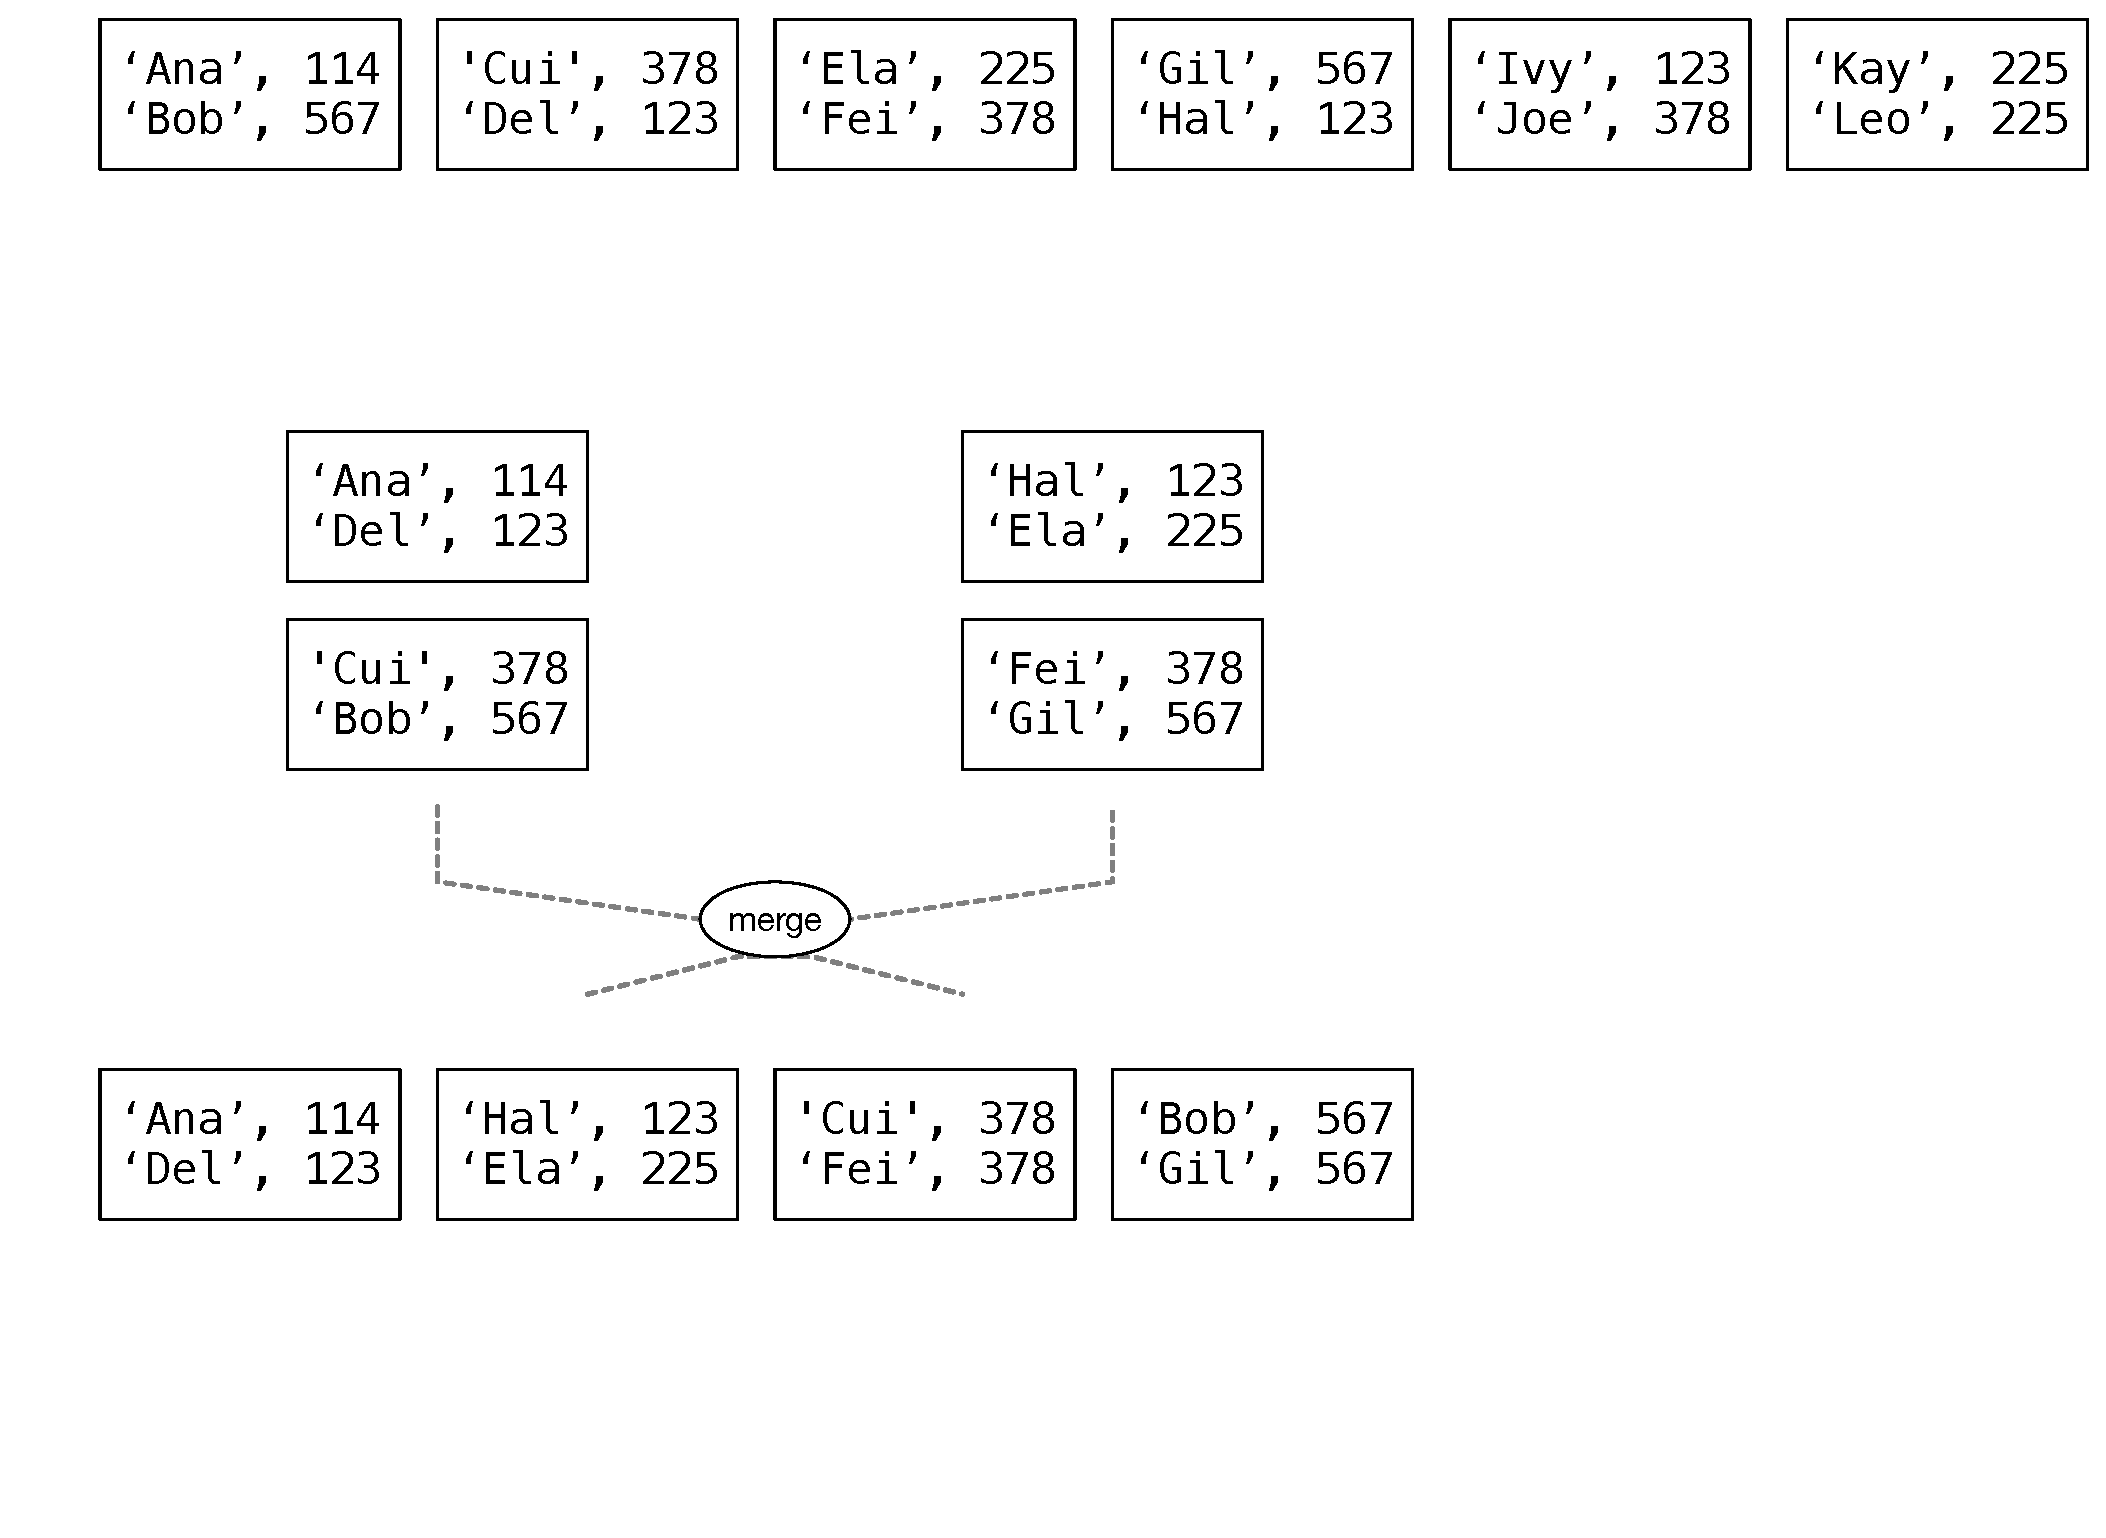
\includegraphics[width=0.9\textwidth]{figures/mergesort_example/step6.eps}};}
\onslide<7|handout:0>{\node at (0,0) {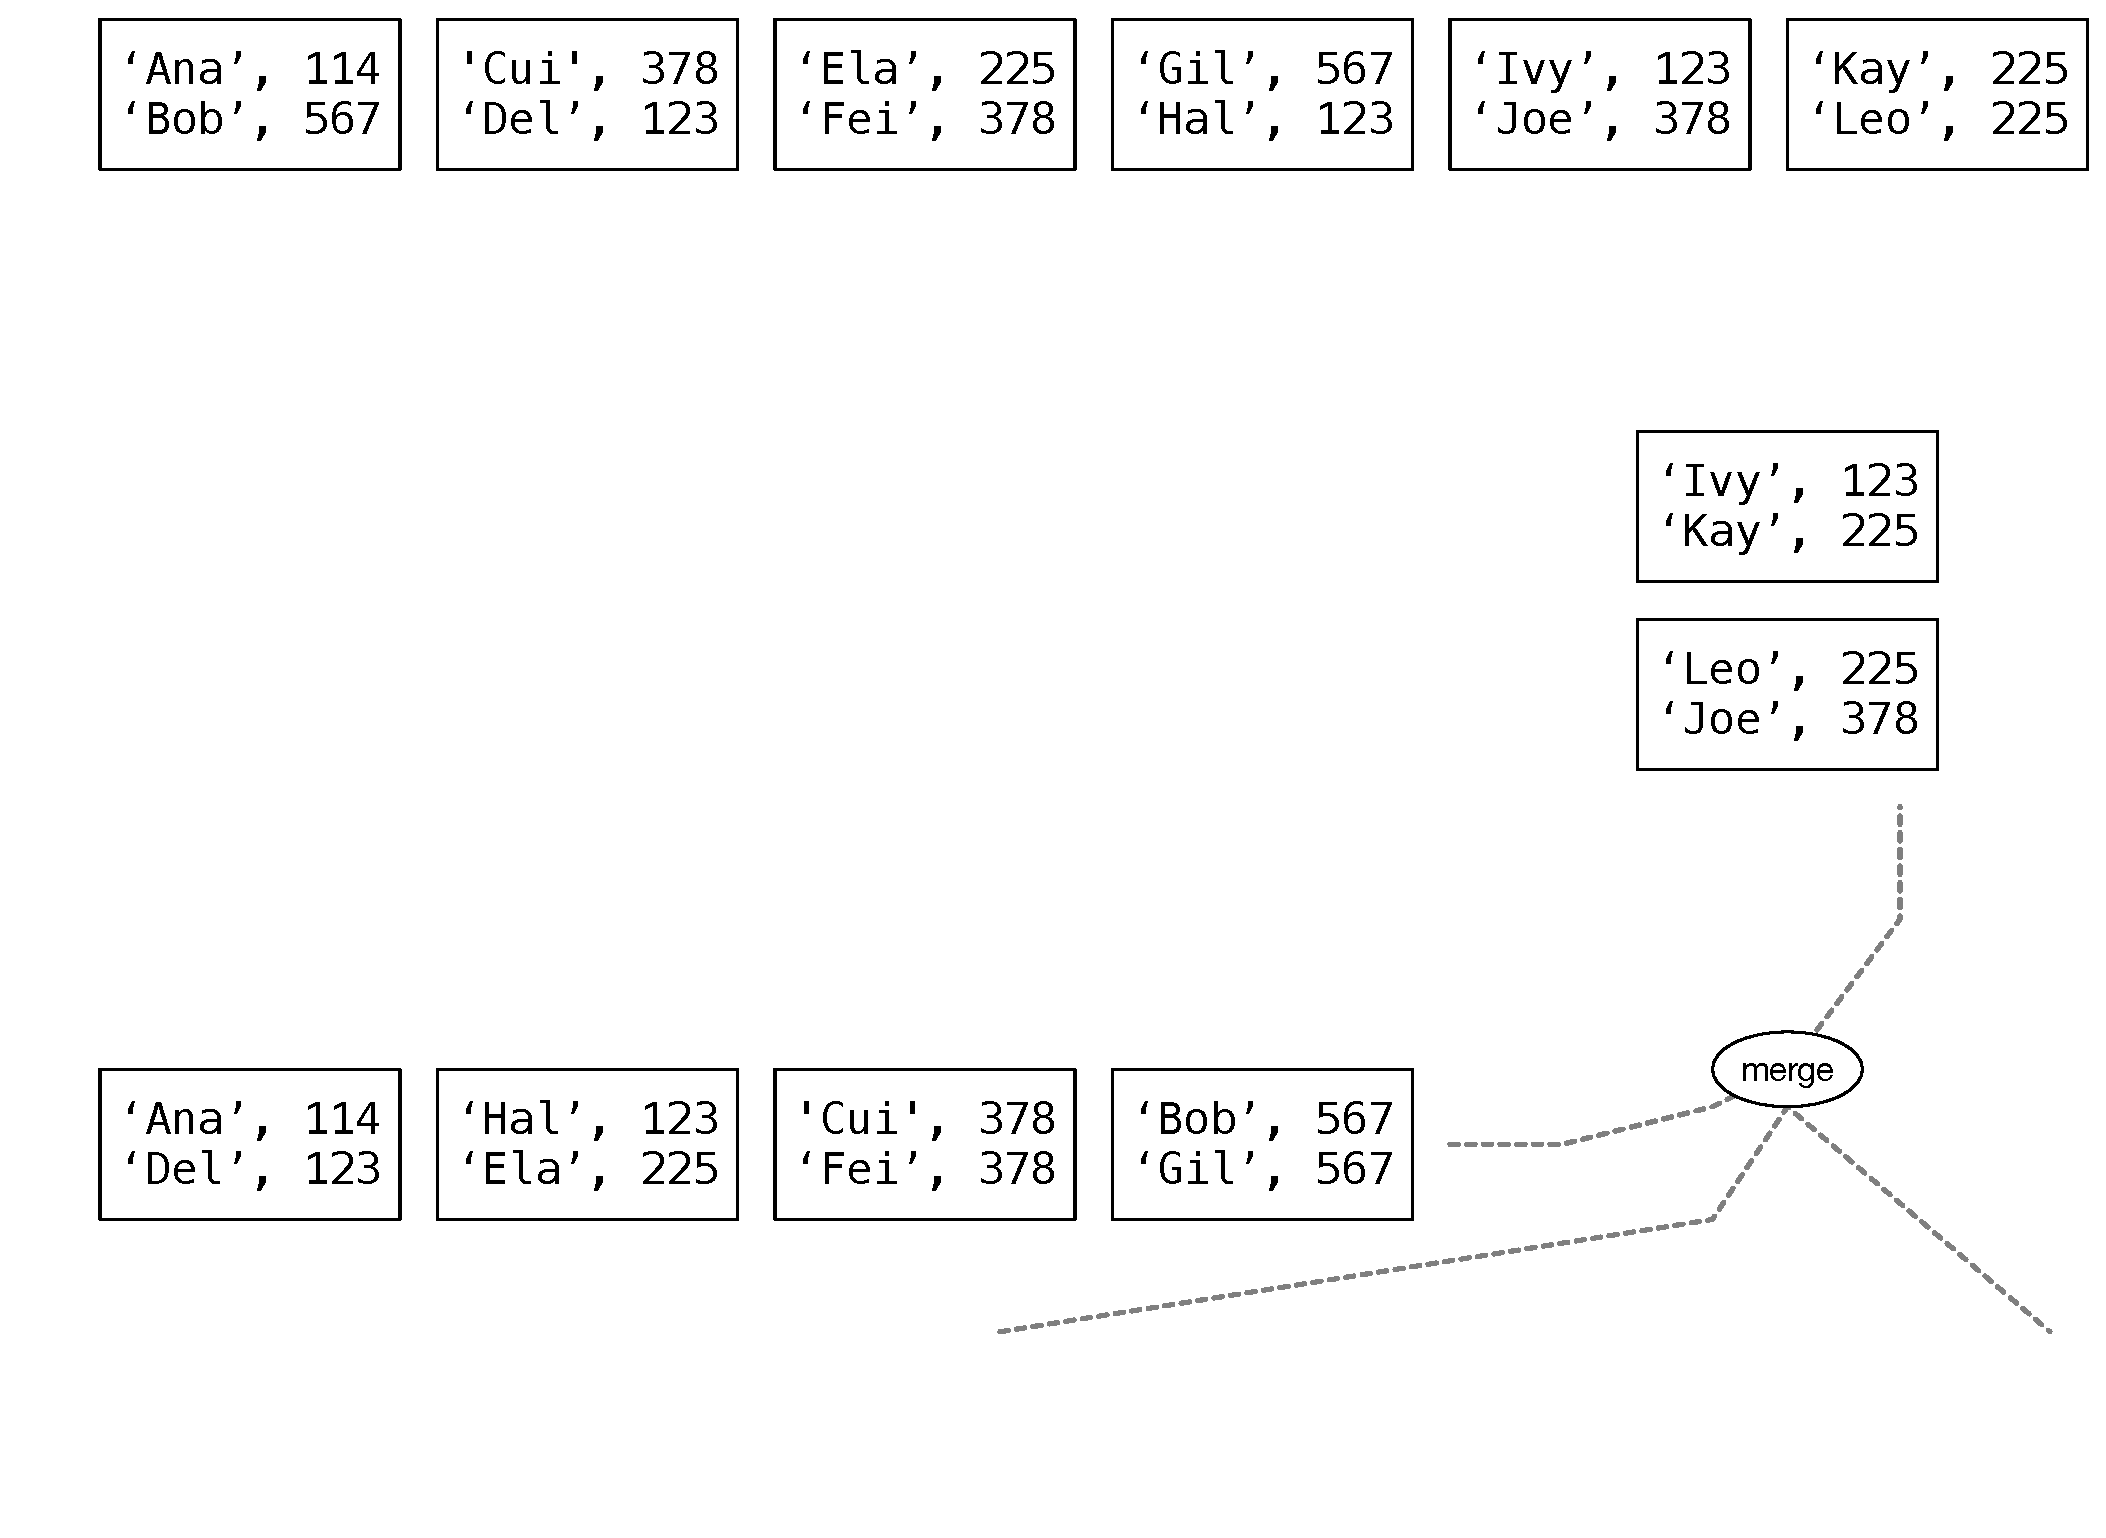
\includegraphics[width=0.9\textwidth]{figures/mergesort_example/step7.eps}};}
\onslide<8|handout:0>{\node at (0,0) {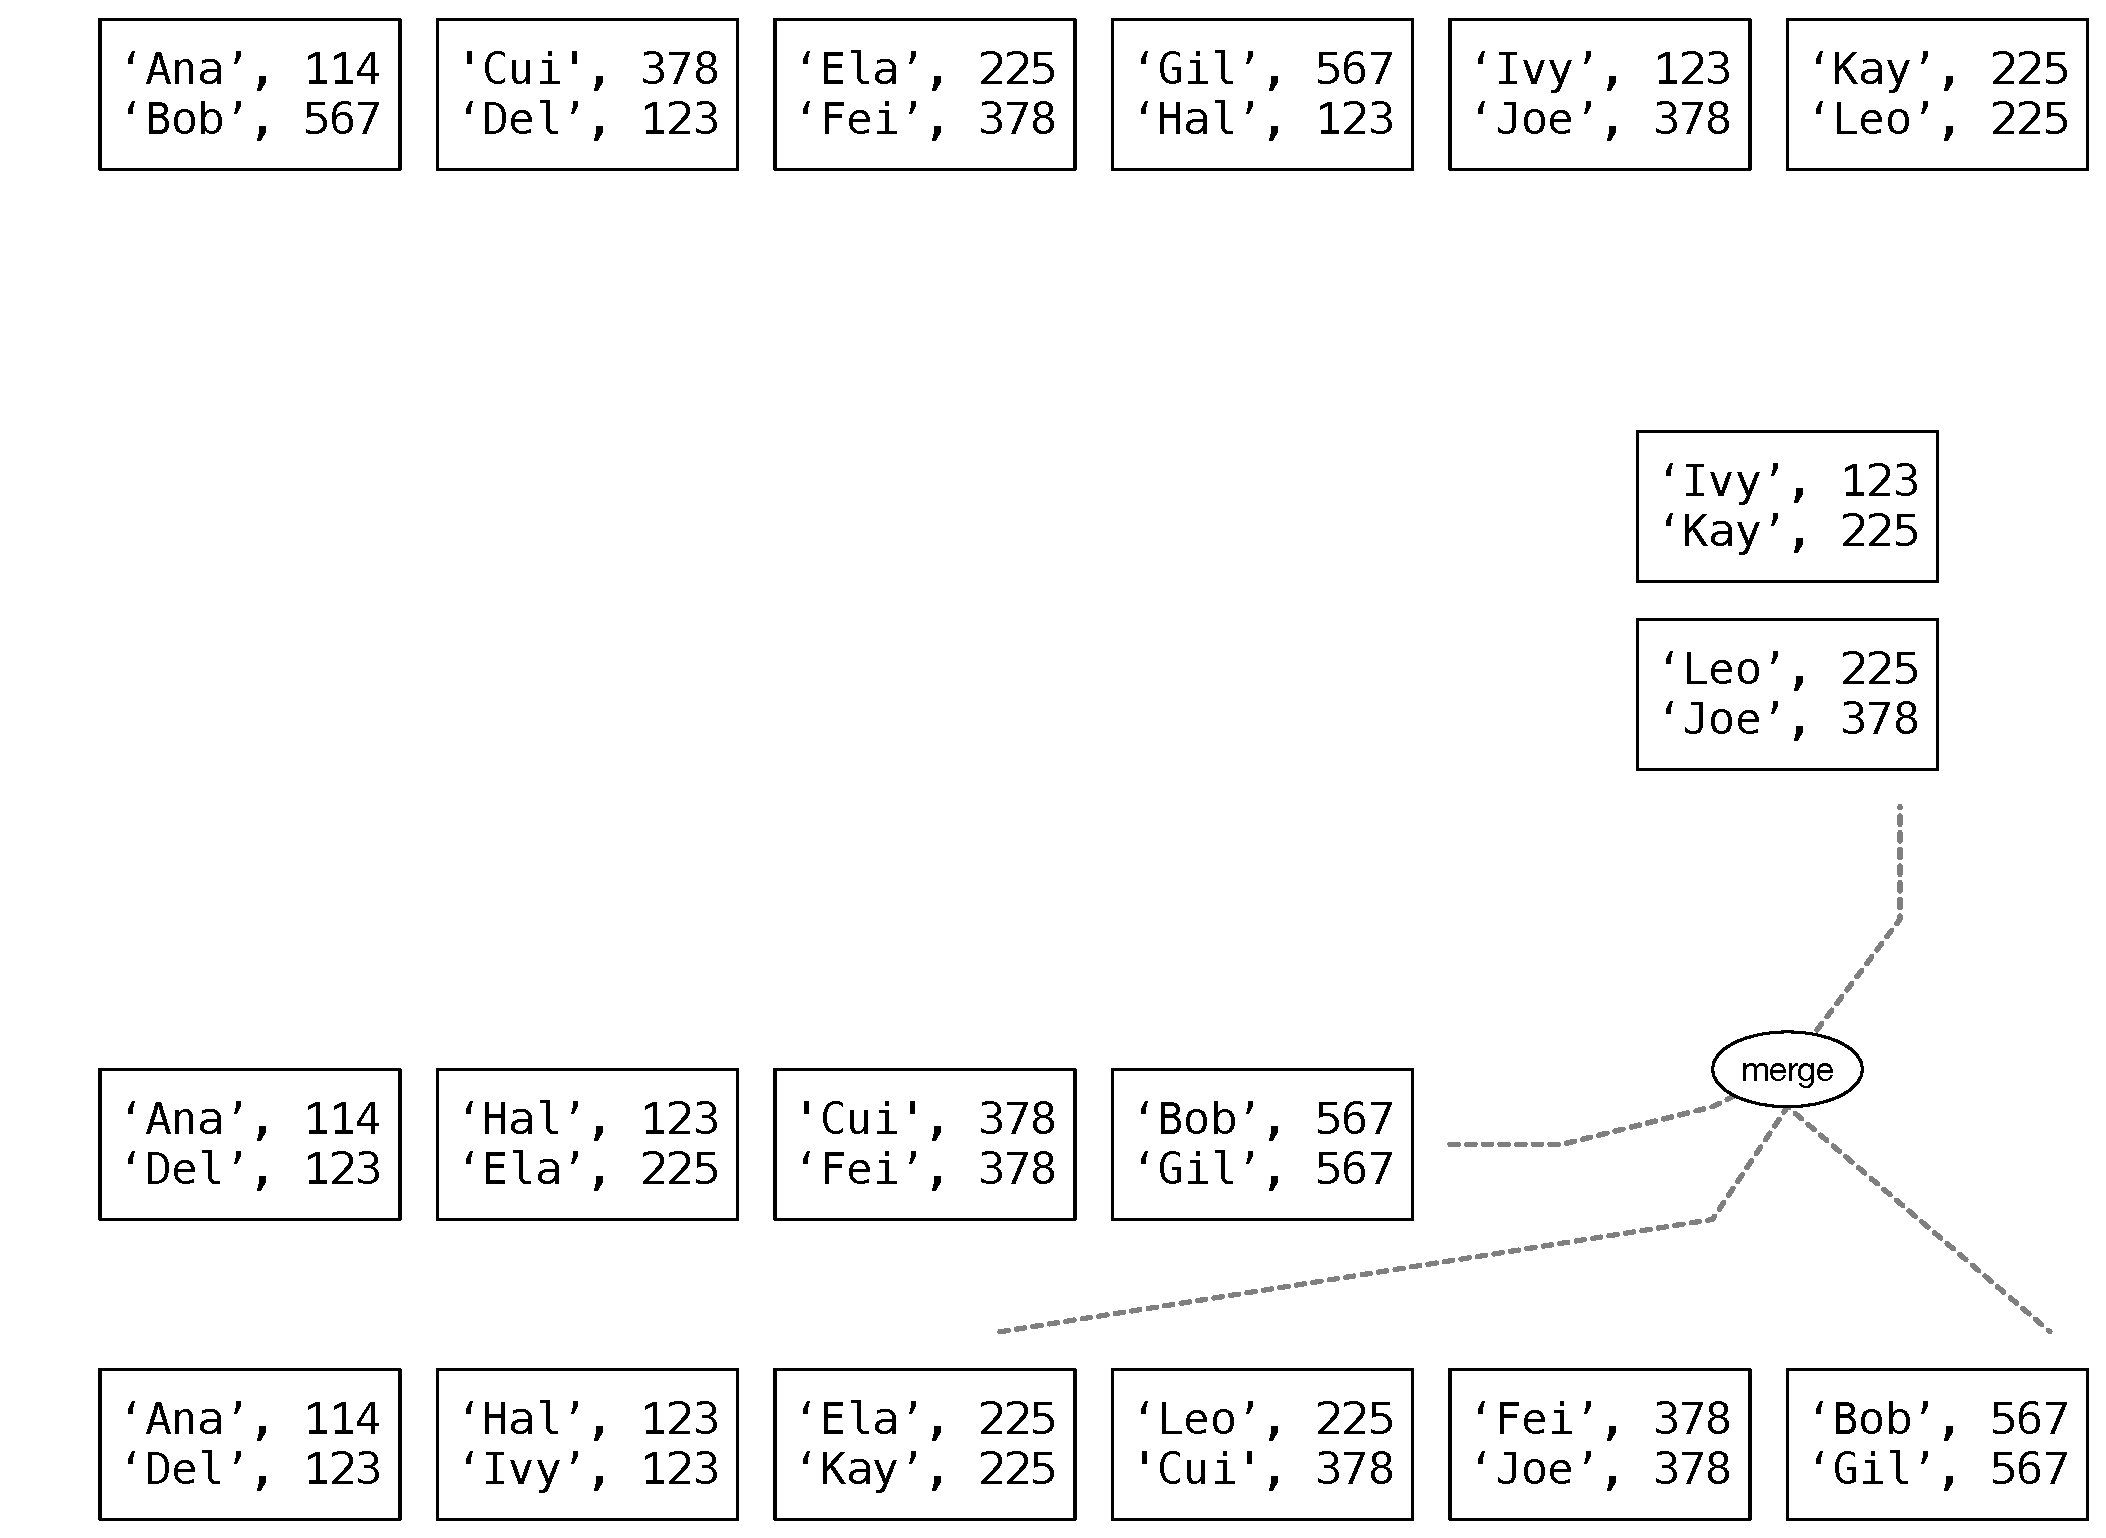
\includegraphics[width=0.9\textwidth]{figures/mergesort_example/step8.eps}};}
\onslide<9|handout:1>{\node at (0,0) {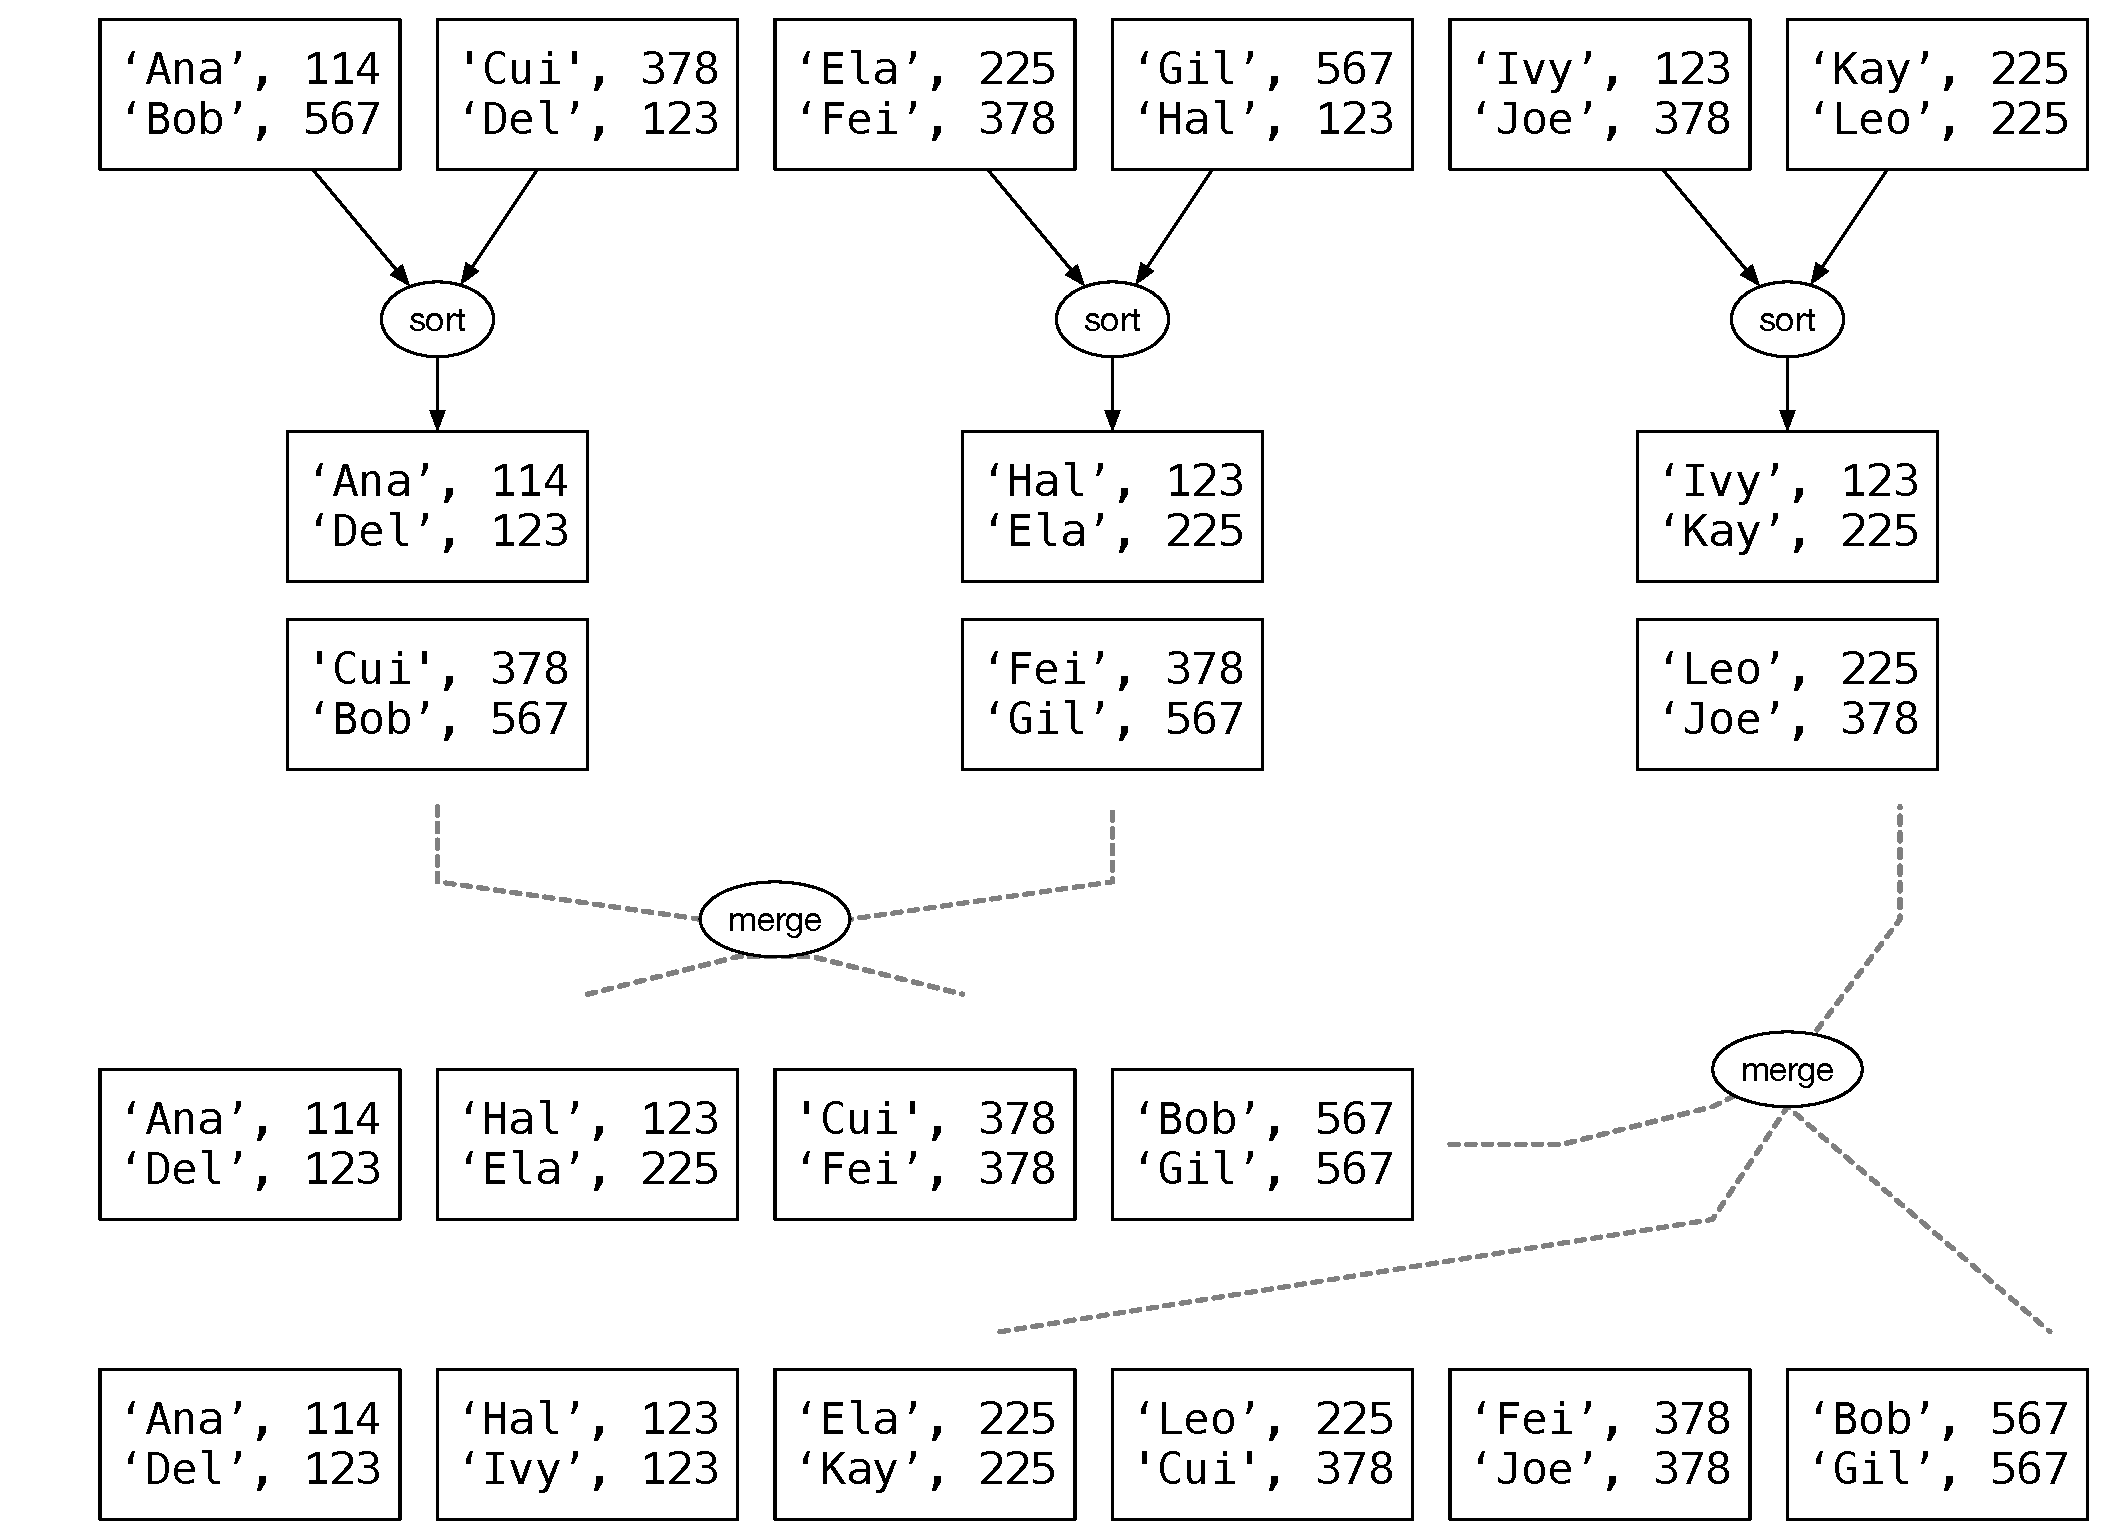
\includegraphics[width=0.9\textwidth]{figures/mergesort_example/final.eps}};}
\end{tikzpicture}
\end{center}

\end{frame}

%
% --------------------------------------------------------------------------
%
\begin{frame}{Sort-based Equality Join $R.a = S.b$}
\label{sort_based_equality_join_idea}

\begin{enumerate}[label=(\arabic*)]
\item Make a sorted copy of $R$ (on \lstinline{R.a}) and another of $S$ (on \lstinline{S.b}) using the external merge-sort algorithm.
\item Scan the two sorted relations looking for tuples that match:
\begin{itemize}%[label=(\roman*)]
\item[$t_{R}$] : current tuple of $R$
\item[$t_{S1}$] : first tuple in $S$ such that $t_R.a = t_{S1}.b$
\item[$t_{S2}$] : current tuple in $S$ such that $t_R.a = t_{S2}.b$
\end{itemize}
\end{enumerate}

\vskip2em

\begin{center}
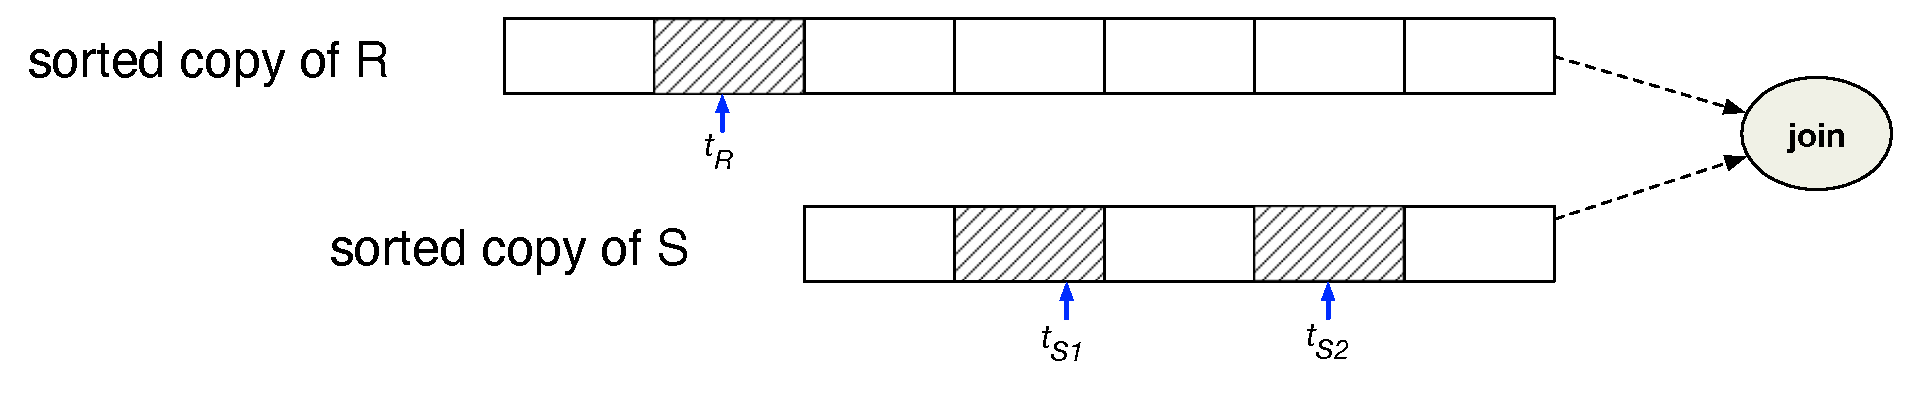
\includegraphics[width=\textwidth]{figures/sort_based_join}
\end{center}
\end{frame}

%
% --------------------------------------------------------------------------
%
\begin{frame}[fragile]

\textbf{Example:} \lstinline[style=SQL]!SELECT name, time FROM Member JOIN Schedule!

\vskip2em

\begin{center}
\begin{tikzpicture}
\node at (-1.05,4) {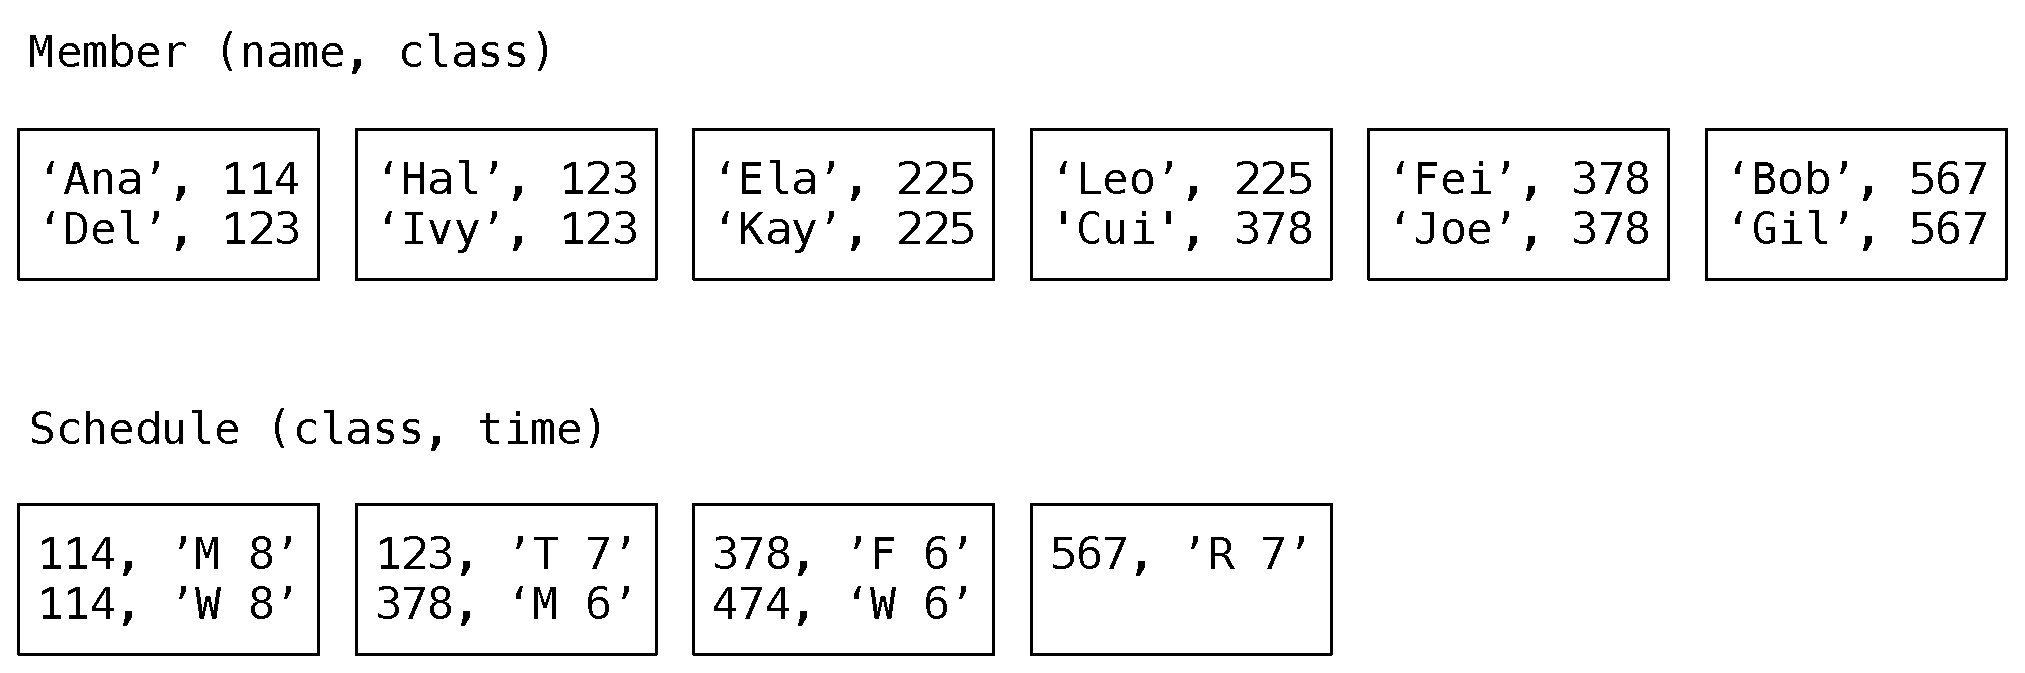
\includegraphics[width=0.85\textwidth]{figures/sort_join/sorted_tables.eps}};
\onslide<1|handout:0>{\node at (0,0) {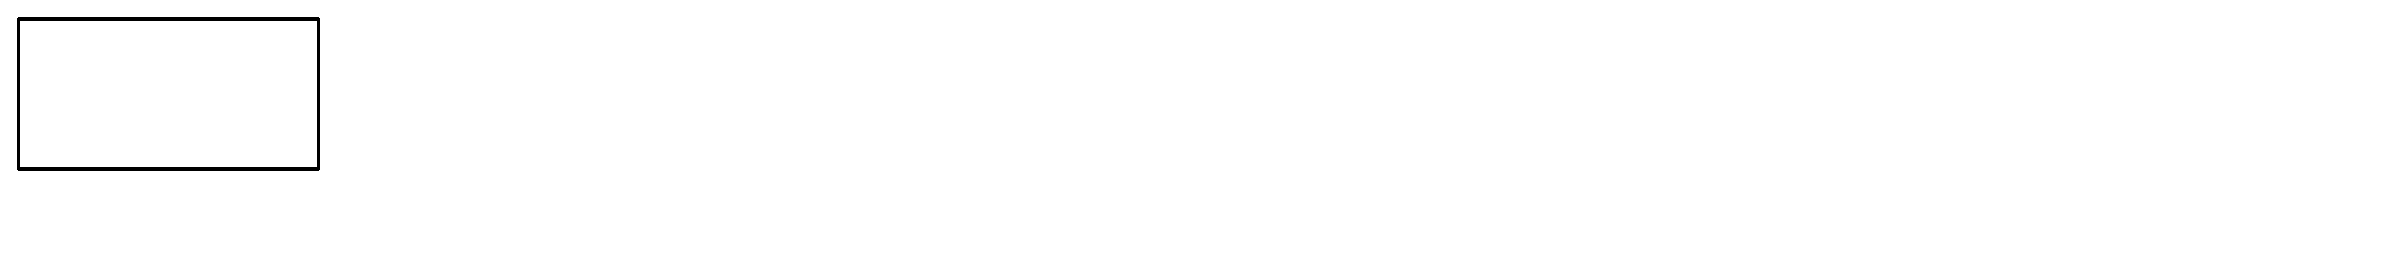
\includegraphics[width=1.05\textwidth]{figures/sort_join/empty_block.eps}};}
\onslide<2|handout:0>{\node at (0,0) {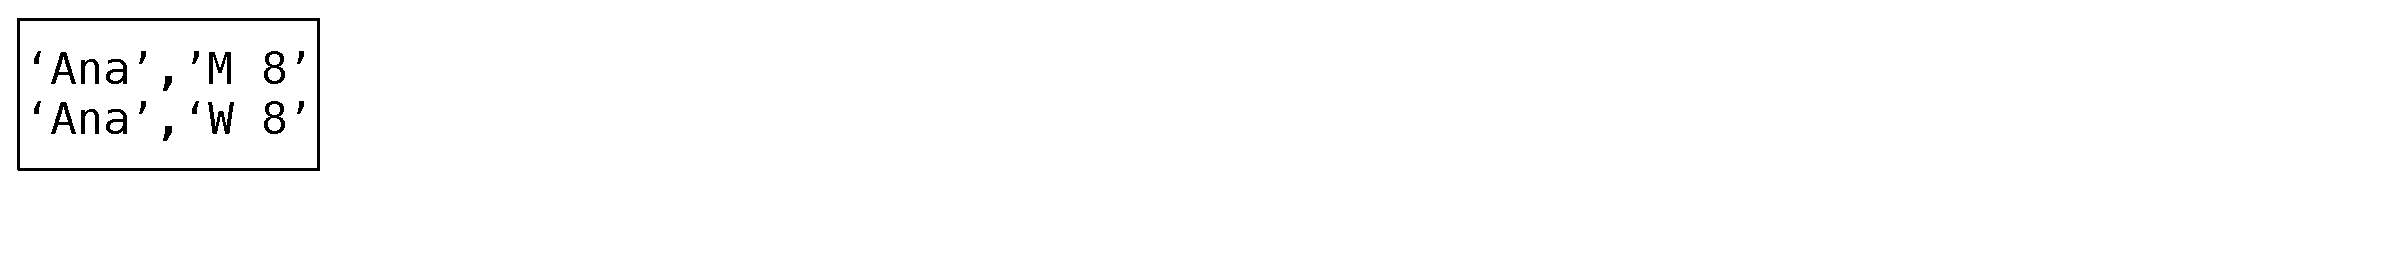
\includegraphics[width=1.05\textwidth]{figures/sort_join/step1.eps}};}
\onslide<3|handout:0>{\node at (0,0) {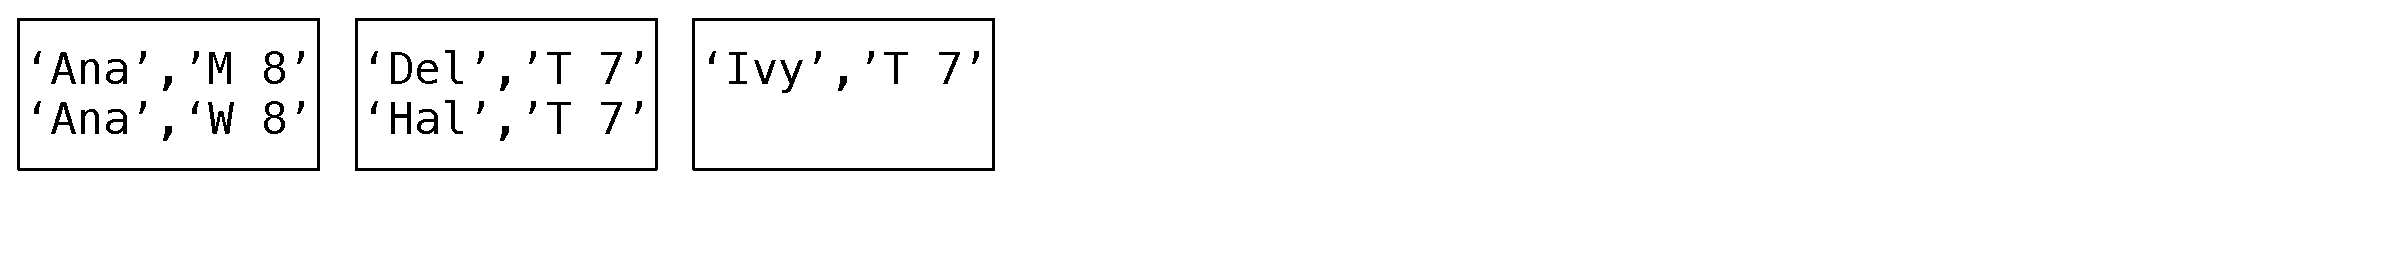
\includegraphics[width=1.05\textwidth]{figures/sort_join/step2.eps}};}
\onslide<4|handout:0>{\node at (0,0) {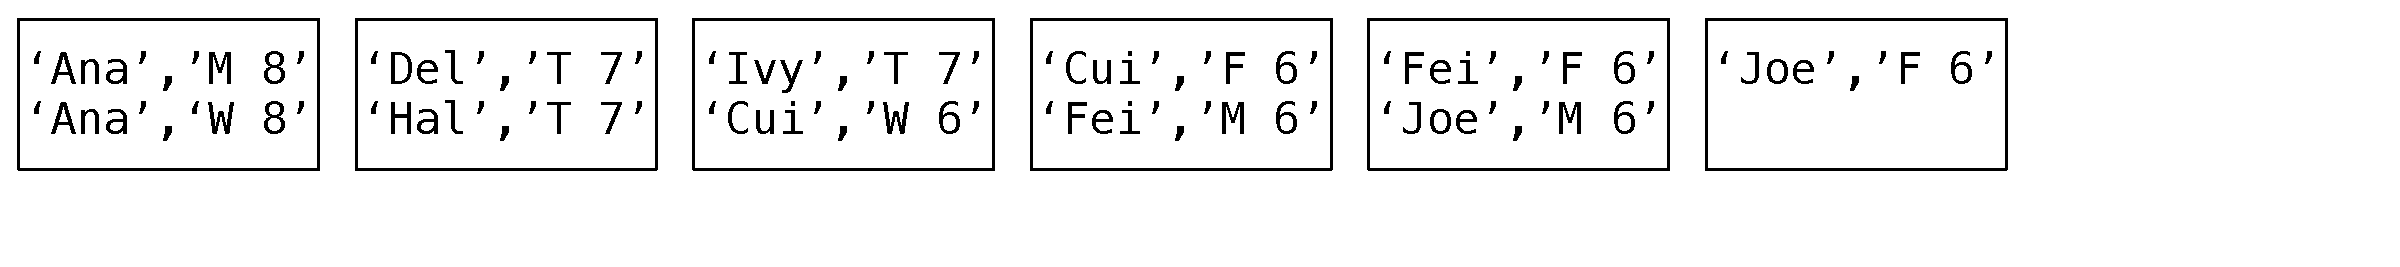
\includegraphics[width=1.05\textwidth]{figures/sort_join/step3.eps}};}
\onslide<6|handout:1>{\node at (0,0) {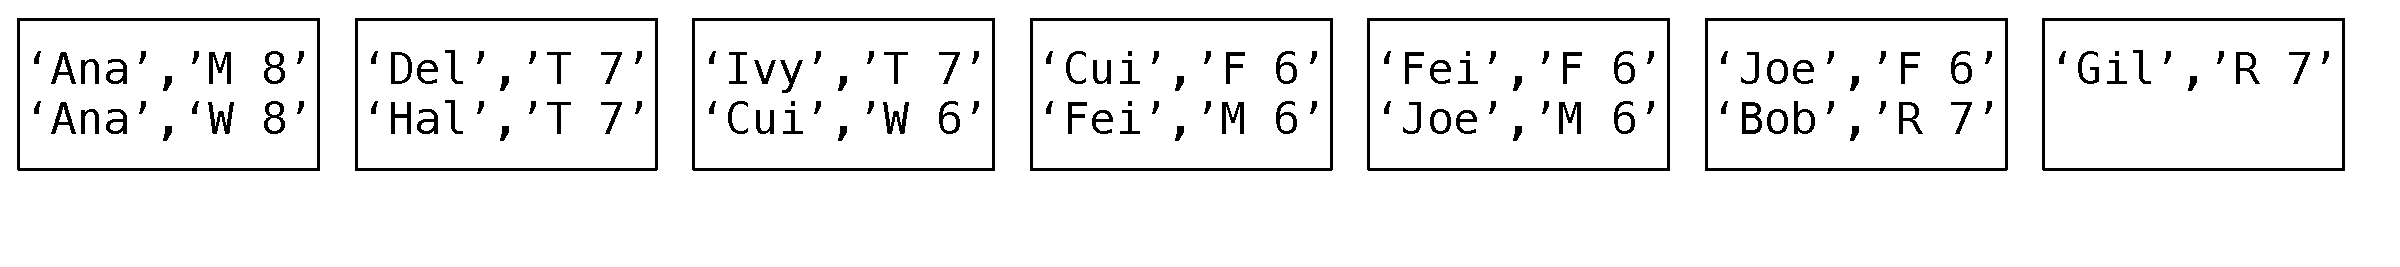
\includegraphics[width=1.05\textwidth]{figures/sort_join/step4.eps}};}
\end{tikzpicture}
\end{center}


\end{frame}


%
% --------------------------------------------------------------------------
%
\begin{frame}[fragile]
\label{sort_based_equality_join}

Pseudo-code of sort-based equality join. For simplicity, we refer to pointers to the tuples inside the sorted files.

\begin{center}
\scalebox{0.75}{\begin{minipage}{1.25\textwidth}%

\begin{algorithm}[H]
\begin{algorithmic}[1]
\caption*{\textbf{Open()} for sort-based evaluation of $R\Join_{R.a=S.b} S$}
\State $t_R \leftarrow $ first tuple in $R$; $t_{S1} \leftarrow $ first tuple in $S$; $t_{S2} \leftarrow t_{S1}$ 
\end{algorithmic}
\end{algorithm}
\end{minipage}}

\vskip0.75em

\scalebox{0.75}{\begin{minipage}{1.25\textwidth}%
\begin{algorithm}[H]
\begin{algorithmic}[1]
\caption*{\textbf{GetNext()} for sort-based evaluation of $R\Join_{R.a=S.b} S$}
	\While {$t_R.a \neq t_{S1}.b$} 
		\State \algorithmicif $t_R.a < t_{S1}.b$ 
			\algorithmicthen\  \alert{advance} $t_R$
			\algorithmicelse\  \alert{advance} $t_{S1}$ ; $t_{S2} = t_{S1}$
	\EndWhile
	\If {\lstinline[style=Python,mathescape]!$t_R = \ $ EOF!} \Comment {stop when there are no more tuples in $R$ to be joined}
		\State \Return \lstinline[style=Python,mathescape]!EOF!
	\EndIf
	\If {$t_R.a = t_{S2}.b$} 
		\State \lstinline[style=Python,mathescape]!$t \leftarrow$ join($t_R$, $t_{S2}$)!
		\State \alert{advance} $t_{S2}$
		\If {\lstinline[style=Python,mathescape]!$t_{S2} = \ $ EOF! \textbf{OR} 
		     \lstinline[style=Python,mathescape]!$t_{S2}.b > t_R.a$!} \Comment {all matches of the current $t_R$ found}
			\State \alert{advance} $t_R$ \Comment {the next call to \textbf{GetNext()} will find matches of the next $t_R$}
		\EndIf
		\State \lstinline[style=Python,mathescape]!yield $\ t$!
	\EndIf

\end{algorithmic}
\end{algorithm}
\end{minipage}}
\end{center}
\end{frame}

%
% --------------------------------------------------------------------------
%
\begin{frame}{Merge-Join on equality $R.a=S.b$}
\label{merge_join_algorithm}

If there are enough buffers to read all chunks of $R$ and $S$ concurrently, one can perform the join itself during the ``merge'' phase on the previous algorithm.

\textbf{Gist:} let $p$ point to the ``smallest'' tuple in $R$; find all matching tuples in $S$ (as in the previous algorithm); advance $p$; repeat.

\vskip1em

\begin{center}
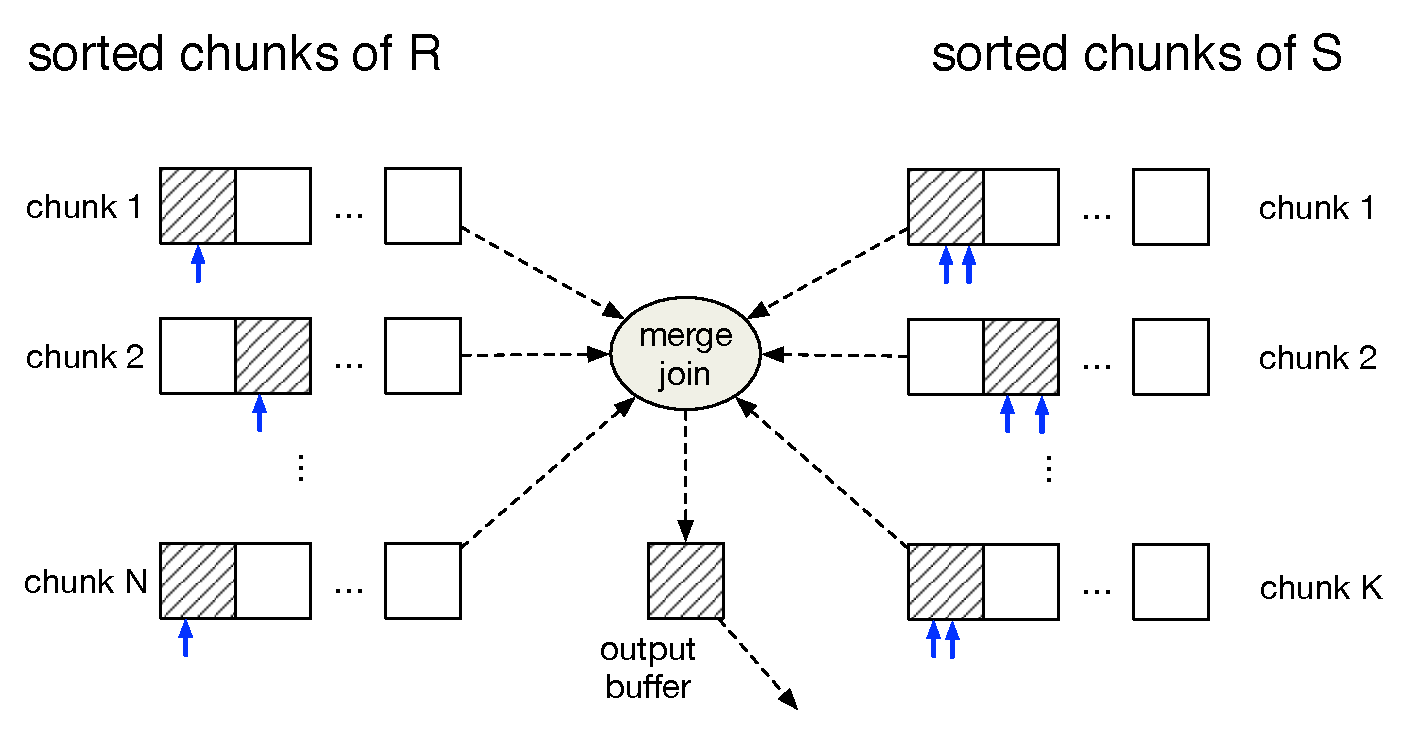
\includegraphics[width=0.75\textwidth]{figures/merge_join.pdf}
\end{center}
\end{frame}


%
% --------------------------------------------------------------------------
%
\begin{frame}
Example of merge-join:

\vskip2em

\begin{center}
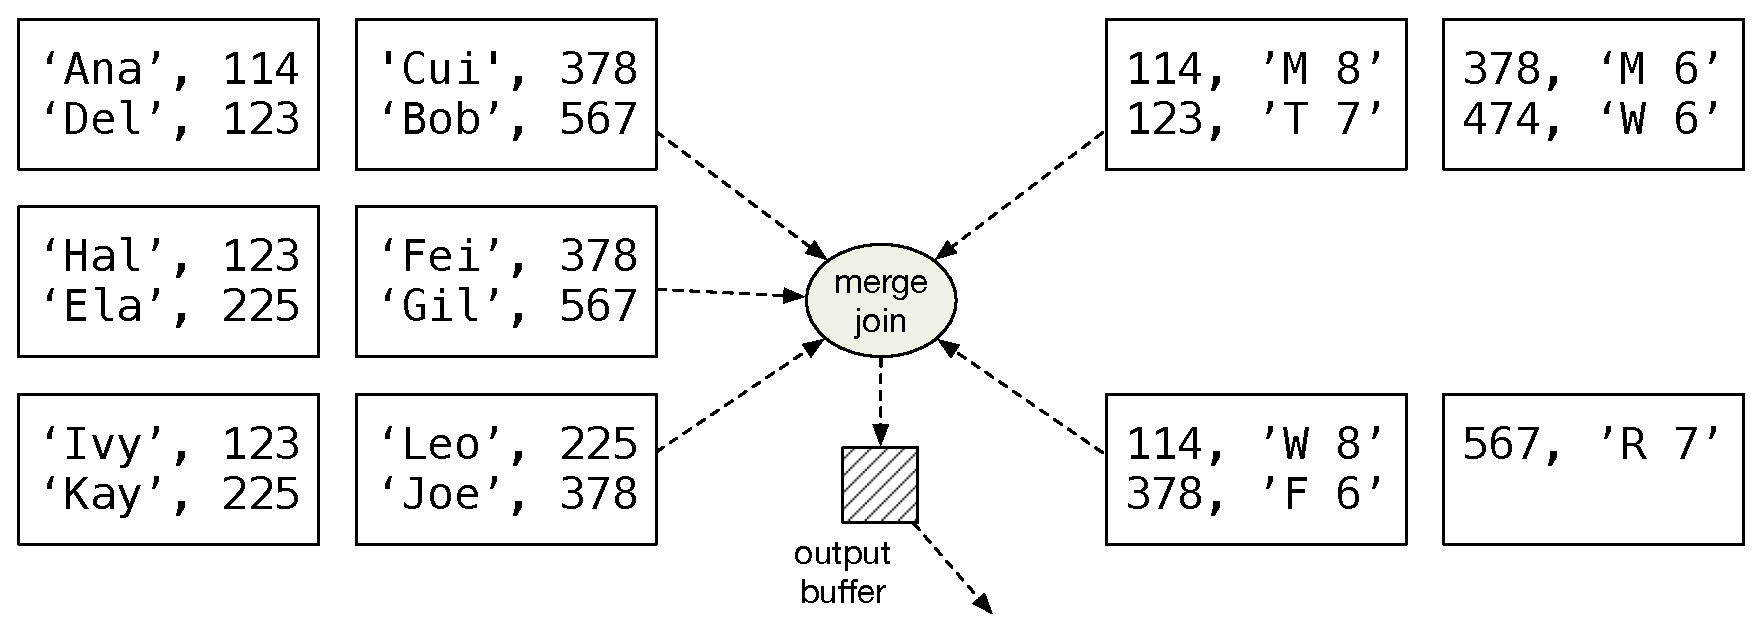
\includegraphics[width=0.9\textwidth]{figures/merge_join_example.eps}
\end{center}

\end{frame}

%
% --------------------------------------------------------------------------
%
\begin{frame}{Sort-based algorithms for other binary operators}
\label{generic_sort_merge_set_operator}

The same ``sort-merge'' framework can be used for the other binary operators.

\textbf{Set Union $R\cup S$}: copy the next ``smallest'' tuple amongst all pointers (in either $R$ and $S$) to the output; advance all pointers to duplicates of that tuple until they point to something else.

\begin{center}
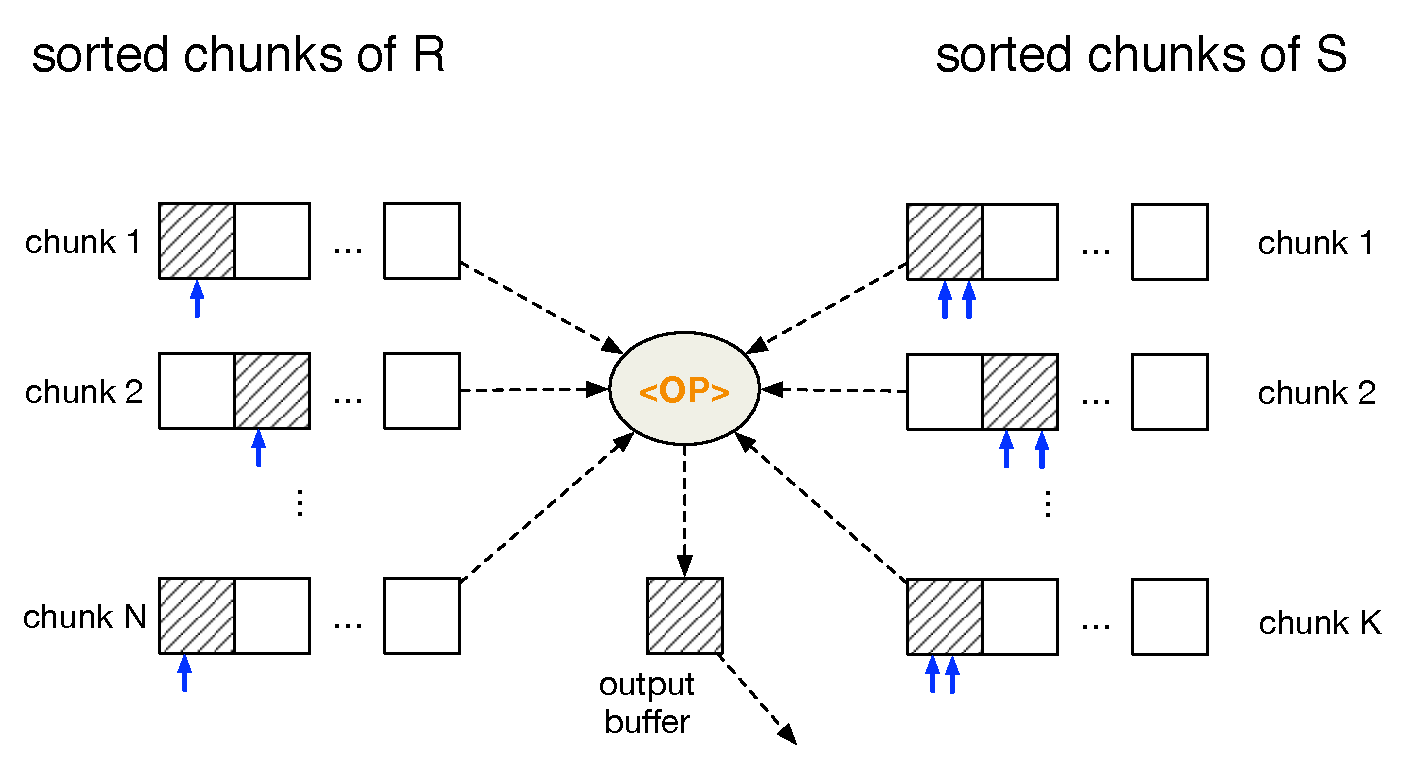
\includegraphics[width=0.75\textwidth]{figures/merge_OP.pdf}
\end{center}
\end{frame}


%
% --------------------------------------------------------------------------
%
\begin{frame}


\textbf{Set Intersection $R\cap S$}: copy the next ``smallest'' tuple that appears in both $R$ and $S$ to the output; advance all pointers to duplicates of that tuple until they point to something else.

\textbf{Set difference $R-S$}: copy the next ``smallest'' tuple in $R$ but not in $S$ (or vice-versa for $S-R$); advance all pointers on $R$ (or $S$, for $S-R$) until a new ``smallest'' tuple is found.

\begin{center}
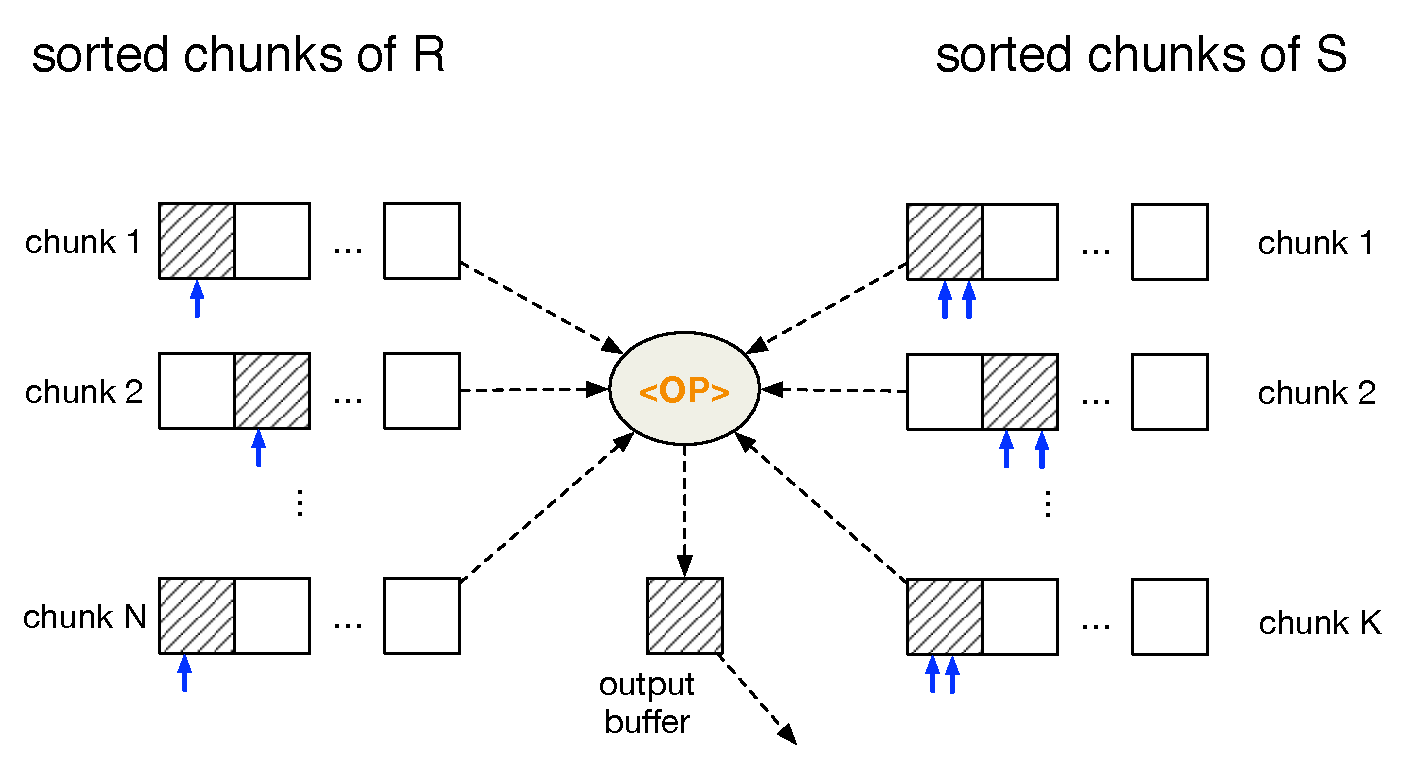
\includegraphics[width=0.75\textwidth]{figures/merge_OP.pdf}
\end{center}
\end{frame}

%%%%%%%%%%%%%%%% ------------------------

\section{Cost Estimation}
%!TEX root = lec05_query_processing.tex

%
% ------------------------------------------------------------------------
%
\begin{frame}{Which plan is better?}

Consider the two following plans that compute the same answer. 

They have the same I/O and memory cost. \blue{Which one will take the least \textbf{time} to execute?}

\vskip3em

\begin{center}
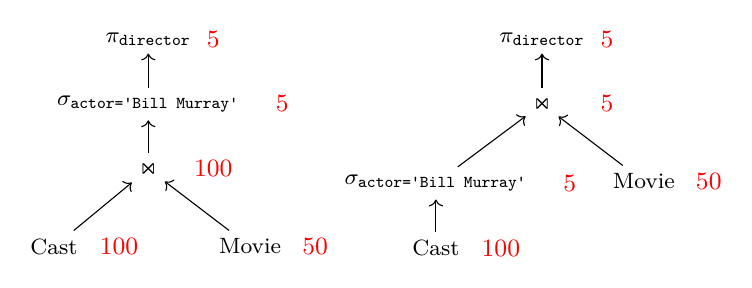
\begin{tikzpicture}[node distance=0.825cm,every node/.style={inner sep=1,outer sep=2,font=\footnotesize}]
    \node (1) at (0,0) {$\pi_{\texttt{director}}$};
    \node (2) [below of=1] {$\sigma_{\texttt{actor='Bill Murray'}}$};
    \node (3) [below of=2] {$\Join$};
    \node (4) [below right= of 3] {\lstinline{Movie}};
    \node (5) [below left= of 3] {\lstinline{Cast}};
    \path[commutative diagrams/.cd, every arrow, every label]
        (2) edge node {} (1)
        (3) edge node {} (2)
        (4) edge node {} (3)
        (5) edge node {} (3);   

    \tikzset{sizeEst/.style={color=red,font=\small}}
    \node [sizeEst,right of=1] {5};
    \node [sizeEst,right = 0.25cm of 2] {5};
    \node [sizeEst,right of=3] {100};
    \node [sizeEst,right of=4] {50};
    \node [sizeEst,right of=5] {100};

    \node (1) at (5,0) {$\pi_{\texttt{director}}$};
    \node (2) [below of=1] {$\Join$};
    \node (3) [below right= of 2] {\lstinline{Movie}};
    \node (4) [below left= 0.6cm and -0.125cm  of 2] {$\sigma_{\texttt{actor='Bill Murray'}}$};
    \node (5) [below of=4] {\lstinline{Cast}};
    \path[commutative diagrams/.cd, every arrow, every label]
        (2) edge node {} (1)
        (3) edge node {} (2)
        (4) edge node {} (2)
        (5) edge node {} (4);

    \tikzset{sizeEst/.style={color=red,font=\small}}
    \node [sizeEst,right of=5] {100};
    \node [sizeEst,right of=3] {50};
    \pause
    \node [sizeEst,right= 0.25cm of 4] {5};
    \pause
    \node [sizeEst,right of=2] {5};
    \node [sizeEst,right of=1] {5};
\end{tikzpicture}
\end{center}
\vskip2em
\end{frame}

%
% ------------------------------------------------------------------------
%
\begin{frame}

The previous example seems trivial: the DBMS can never do worse by performing the selection $\sigma_{\texttt{actor='Bill Murray'}}$ before the join.

\vskip1em

Sometimes the DBMS faces choices which are far from trivial.

\alert{Example 1:} if a query joins 3 tables $R, S, T$, should they be joined like this $(R\Join S)\Join T$? Or is there a better ordering?


\alert{Example 2:} if there exists a secondary index on a table, should it be used or should the DBMS scan the table instead?

\vskip2em

The next slides look into how the DBMS can choose a plan among several alternatives.

\end{frame}

%
% ------------------------------------------------------------------------
%
\begin{frame}{Result sizes and query time}

As we just saw, two plans for the same query, with the same I/O and memory cost can have different execution time, depending on the number of tuples that are computed by intermediate results.

However, the DBMS cannot execute various plans to know the exact size of their intermediate results.

\vskip1em

Instead, the DBMS needs to \textbf{estimate} those sizes for any given plan, using statistics about the database.

\begin{BOX}{Estimated vs Real Cost}
Using estimated costs, the DBMS can evaluate many candidate plans in less time than it would take to execute any of them. In practice estimated cost is correlated with actual cost.
\end{BOX}

\end{frame}

%
% ------------------------------------------------------------------------
%
\begin{frame}{Database statistics}
\label{dbms_table_statistics}
The following are the simplest statistics (per relation $R$ in the database) the DBMS can use to estimate the cost of a query plan.

\begin{center}
\begin{tabular}{rl}
$B(R)$& number of of blocks to hold all tuples in $R$ \\
$T(R)$ & number of tuples in $R$ \\
$S(R)$ & number of of bytes per tuple in $R$ \\
$V(R, a)$ & number of distinct values of $a$ in $R$
\end{tabular}
\end{center}

\vskip1em

The DBMS might also keep the lowest and the highest values of numeric attributes:

\begin{center}
\begin{tabular}{rl}
$\MIN(R, a)$ & lowest value of $a$ in $R$\\
$\MAX(R, a)$ & highest value of $a$ in $R$
\end{tabular}
\end{center}


\end{frame}

%
% ------------------------------------------------------------------------
%
\begin{frame}

\begin{columns}[onlytextwidth]
\begin{column}{0.375\textwidth}
\textbf{Example}
\vskip2em

\small
Assume:\\
- \lstinline[style=C]{sizeOf(int)} = 4 bytes\\
- \lstinline[style=C]{sizeOf(char)} = 2 bytes\\
- \lstinline[style=C]{sizeOf(float)} = 8 bytes
\end{column}
\begin{column}{0.6\textwidth}
\scalebox{0.75}{\usebox{\SimplifiedMovieTableDDL}}
\vskip1em
\scalebox{0.75}{\usebox{\MovieTable}}
\end{column}
\end{columns}

\vskip2em

\small
\begin{tabular}{l|l|l}
$T(\texttt{Movie}) = 5$ & $V(\texttt{Movie}, \texttt{title}) = 4$ & $\MIN(\texttt{Movie}, \texttt{year}) = 1984$\\
$S(\texttt{Movie}) = 92$ & $V(\texttt{Movie}, \texttt{year}) = 5$ & $\MAX(\texttt{Movie}, \texttt{year}) = 2016$\\
 & $V(\texttt{Movie}, \texttt{imdb}) = 4$ & $\MIN(\texttt{Movie}, \texttt{imdb}) = 5.3$\\
 & $V(\texttt{Movie}, \texttt{director}) = 5$ & $\MAX(\texttt{Movie}, \texttt{imdb}) = 8.1$\\
\end{tabular}
\normalsize
\end{frame}


%
%
%
\begin{frame}{Result Size Estimation}

To estimate the size of a query or sub-expression $Q$ we need to know $T(Q)$ and $S(Q)$. 

Since memory buffers have a fixed size, we can always estimate the number of buffers (and thus how much RAM) is needed as 
\[B(Q)=\ceil*{\frac{T(Q)\cdot S(Q)}{\text{buffer size}}}\]

\vskip1em

For simplicity, we consider here the cases where all tuples are of fixed size. For variable-sized tuples, the DBMS can use the average tuple size, for example, to get a reasonable estimate.

\end{frame}

%
% ------------------------------------------------------------------------
%
\begin{frame}{Estimates with Selections}

Let $Q: \sigma_{a_i=v}(R)$. 

What are good estimates for $S(Q)$ and $T(Q)$ and $V(Q,\cdot)$?
\begin{align*}
S(Q) &= S(R) \ \ \ \alert{^\dagger}\\
V(Q,a_i) &= 1 \ \ \alert{^\ddagger}\\
V(Q,a_j) &= V(R,a_j) \qquad j\neq i
\end{align*}

\vskip1em 

$\alert{^\dagger}$ Since the selection does not change the tuples.

$\alert{^\ddagger}$ For numeric attributes we can do better by checking if $\MIN(R,a_i) \leq v \leq\MAX(R,a_i)$ and assume 0 otherwise. For non-numeric attributes, such analysis is much harder.

\end{frame}


%
% ------------------------------------------------------------------------
%
\begin{frame}

What about $T(Q)$? How many tuples of $R$ should have $a_i=v$? 

\vskip1em

\begin{block}{\blue{Predicate selectivity}}
The selectivity of predicate $c_i$ is defined as \[s(R,c_i)=\frac{T(\sigma_{c_i}(R))}{T(R)}\]
and estimated as in the previous slides.
\end{block}


\vskip1em

In general, $T(\sigma_{c_i}(R)) = \ceil*{s(R, c_i)\cdot T(R)}$, for any expression $R$ (not just base tables).

\end{frame}

\begin{frame}

\textbf{\blue{Estimating} predicate selectivity}:

\vskip1em

We \alert{need to make assumptions} about how the values are distributed in order to make any estimates. 

One common assumption in cost estimation is that the values are \textbf{uniformly distributed} across the table, meaning that, for any given attribute $a_i$:
\begin{itemize}[-,topsep=-0.5em,noitemsep]
\item All $V(R,a_i)$ distinct values appear the same number of times.
\item All values are \emph{equally likely} to appear in any given tuple $t$.
\end{itemize}

\vskip2em
 
Thus:  \qquad \fbox{$s(R, \sigma_{a_i = v}) = \frac{1}{V(R, a_i)}; \qquad T(Q)= \ceil*{\frac{1}{V(R,a_i)} \cdot T(R)}$}.

\end{frame}

%
% ------------------------------------------------------------------------
%
\begin{frame}[fragile]

An alternative estimate is to assume all values \underline{in the domain} are \alert{equally likely}. This, of course, only makes sense for attributes with a discrete domain. 

In this case, we'd have $s(R, a_i=v)= \frac{1}{|\text{domain}(a_i)|}$

\vskip1em

\textbf{Example:}

\begin{center}
\begin{lstlisting}[style=SQL,basicstyle=\ttfamily\footnotesize]
CREATE TABLE Instructor(name TEXT, faculty TEXT, email TEXT, 
    CHECK (faculty IN ('Arts','Science','Engineering',
                       'Business','Law','Medicine')));
\end{lstlisting}
\end{center}

$T(\sigma_{\texttt{faculty='Arts'}}(\texttt{Instructor}))= \ceil*{\frac{1}{6} \cdot T(\texttt{Instructor})}$

\vskip1em

The estimate is always the same for values that belong to the domain, and 0 for values not in the domain.


\end{frame}


%
% ------------------------------------------------------------------------
%
\begin{frame}[fragile]{Selections With Ranges}

When the selection in based on a range of values $Q=\sigma_{a_i > v}(R)$ the estimates for $T(Q)$ and $V(Q,a_i)$ need to be adjusted.

With \emph{low}/\emph{high} statistics, we can make some reasonable estimates. If $\MIN(R,a_i)\leq v \leq \MAX(R,a_i)$\footnote{The boundary cases when $v$ is out of that range are left as an exercise.}, we can use:

\[
T(Q) = \ceil*{\frac{\MAX(R,a_i)-v}{\MAX(R,a_i)-\MIN(R,a_i)}T(R)} \text { and }\]
\[V(Q,a_i) = \ceil*{\frac{\MAX(R,a_i)-v}{\MAX(R,a_i)-\MIN(R,a_i)}V(R,a_i)}\]

Estimates for $Q=\sigma_{a_i < v}(R)$ are computed analogously.

\vskip1em

\end{frame}

%
% ------------------------------------------------------------------------
%
\begin{frame}

\textbf{Example:} $Q=\sigma_{\texttt{imdb>7} }(\texttt{Movie})$.

\[T(Q) = \ceil*{\frac{\textcolor{red}{8.1}-\alert{7}}{\textcolor{red}{8.1}-\textcolor{blue}{5.3}}\ T(\texttt{Movie})} = \ceil{1.96} =2\]

\[V(Q,\texttt{imdb}) = \ceil*{\frac{\textcolor{red}{8.1}-\alert{7}}{\textcolor{red}{8.1}-\textcolor{blue}{5.3}}\ V(\texttt{Movie},\texttt{imdb})} = \ceil{1.57} =2\]

\vskip1em

\begin{block}{}
These estimates are not great because the imdb values are \textbf{not} uniformly distributed. We would need better statistics to be more accurate here.
\end{block}

\end{frame}

%
% ------------------------------------------------------------------------
%
\newsavebox{\histogramExample}
\savebox{\histogramExample}{
    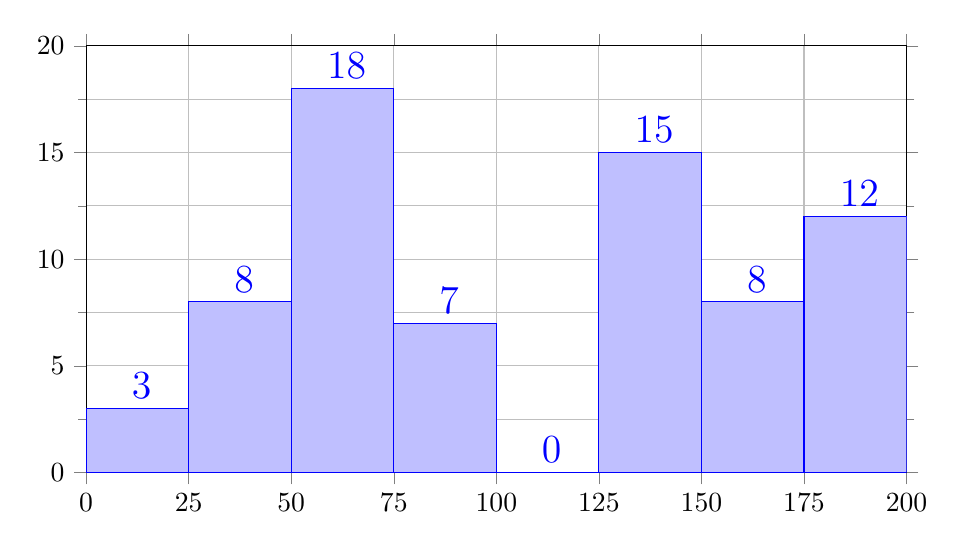
\begin{tikzpicture}
        \begin{axis}[
            height=7cm,
            width=12cm,
%            ybar interval,      % <-- this causes the `xticks' to be centered
            ymin=0,ymax=20,
            xmin=0,xmax=200,
            grid=both,
            minor y tick num=1,
            yminorgrids=true,
            xtick distance={25},
            tick align=outside, % <-- this positions the ticks "outside"
         ]
            \addplot+ [
                ybar interval,
                mark=none,
                fill=blue!25,   % fill the bars again
                nodes near coords,
                every node near coord/.append style={font=\Large,xshift=20},
            ] coordinates {
                (0,3)(25,8)(50,18)(75,7)(100,0)
                (125,15)(150,8)(175,12)
            };
            \addplot [ybar interval, % the second plot is needed to hide the
              % count of zero in the last bin.
                mark=none,
                color=blue,
                fill=blue!25,   
            ] coordinates {(175,12) (200,0)};
        \end{axis}
    \end{tikzpicture}
}

\begin{frame}{Better estimations with histograms}

\emph{Histograms} are statistical summaries of data that record the number of values that fall within predefined \textbf{bins}. 

In an \emph{equi-width} histogram, all bins have the same width, and cover the same number of elements in the domain.

\begin{center}
\scalebox{0.75}{
\begin{tikzpicture}
\node at (0,0) [anchor=north west] {\scalebox{0.5}{\usebox{\histogramExample}}};
\draw [color=accent,decorate,decoration={brace,amplitude=8pt,raise=3pt},yshift=0pt]
		(0.15,-3.15) -- (0.15,-0.25) node [midway,xshift=-1cm] {\small counts};

\draw [color=accent,decorate,decoration={brace,amplitude=8pt,raise=-3pt},yshift=0pt]
		(5.75,-3.5) -- (0.5,-3.5) node [midway,yshift=-0.35cm] {\small bins};

\draw [red] (3.75,-0.885) rectangle (4.5,-3);

\node (0) [red] at (8,-0.5) {
	\begin{minipage}{2.25cm}\baselineskip=0.75\baselineskip \centering\small
		15 values $125 \leq x <150$
	\end{minipage}
		};
\draw [red,->] (0) -- (4.56,-1);
\end{tikzpicture}}
\end{center}

We can estimate the the probability of a tuple satisfying a selection condition with a histogram of the attribute in the selection.


\end{frame}

%
% ------------------------------------------------------------------------
%
\begin{frame}

\begin{columns}[onlytextwidth]
\begin{column}{0.5\textwidth}

\[
s(R, a_i=x) = \frac{\mathit{count}(\mathit{bin}(x))}{T(R)}
\]

\vskip1em

\textbf{Examples:}
\begin{itemize}[-,noitemsep,topsep=-0.5em]
 \item $s(R, a_i=180)= 12/71$
 \item $s(R, a_i=60)= 18/71$
 \item $s(R, a_i=110)= 0$
\end{itemize}

\end{column}
\begin{column}{0.5\textwidth}
\begin{center}\scalebox{0.75}{
\begin{tikzpicture}
\node at (0,0) [anchor=north west] {\scalebox{0.5}{\usebox{\histogramExample}}};
\draw [color=accent,decorate,decoration={brace,amplitude=8pt,raise=3pt},yshift=0pt]
        (0.15,-3.15) -- (0.15,-0.25) node [midway,xshift=-1cm] {\small counts};

\draw [color=accent,decorate,decoration={brace,amplitude=8pt,raise=-3pt},yshift=0pt]
        (5.75,-3.5) -- (0.5,-3.5) node [midway,yshift=-0.35cm] {\small bins};
\end{tikzpicture}}
\end{center}
\end{column}
\end{columns}

\vskip2em

\textbf{For \alert{ranges}}, sum-up across bins overlapping with the range:
\begin{itemize}[-, noitemsep, topsep=-0.5em]
\item  $s(R, a_i \geq 100)= (0+15+8+12)/71$
\item  $s(R, 10\leq a_i <50)= (3+8)/71$
\end{itemize}

\vskip1em

For $V(Q,a_i)$ we can use either the number of values in the range (as before) or the sum of counts in the respective bins, whichever is smaller.

\end{frame}


\begin{frame}[fragile]

Histograms are an example of how \alert{better statistics offer more accurate predictions}.

The \blue{trade-off} is keeping the histogram up-to-date.
\begin{itemize}[-,topsep=-0.5em]
\item Update the histogram after every database update \textbf{or} only when the database goes offline for maintenance?
\end{itemize}

\vskip1em

\alert{What about textual attributes?}

Histograms defined by equally-spaced strings (e.g., "A", "C", "E", ...) could help with equality queries... but not \emph{wild-card queries}:

\begin{center}
\begin{lstlisting}[style=SQL]
SELECT title, imdb 
FROM Movie 
WHERE title LIKE "%space%"
\end{lstlisting}

\end{center}

Getting accurate estimates is not easy!

\end{frame}

%
% ------------------------------------------------------------------------
%
\begin{frame}

\vskip1em

What about $Q =  \alert\sigma_{\alert{c_1 \wedge \cdots \wedge c_n}}(R)$?

How many tuples satisfy \underline{all of the conditions} at the same time? This can be estimated with a bit of probability theory.

% \end{frame}

% \begin{frame}

Using $s(R, c_i)$ as the probability that a tuple in $R$ satisfies $c_i$, and assuming attribute values are \emph{independent} of each other, we have

\[
T(\sigma_{c_1 \wedge \cdots \wedge c_n}(R)) = \ceil*{\left( \prod_{1\leq i \leq n} s(R,c_i) \right) T(R)}
\]

\vskip1em

\textbf{Example:} $Q=\sigma_{\texttt{imdb>7 } \wedge \texttt{ year=2016}}(\texttt{Movie})$.

\begin{align*}
T(Q) = \ceil*{\left(\frac{2}{5} \cdot \frac{1}{5}\right) \cdot 5} = \ceil*{\frac{2}{5}} = 1
\end{align*}
\end{frame}


\begin{frame}

\vskip1em

Also using $s(R,c_i)$ as the probability that a tuple in $R$ satisfies $c_i$, and assuming attribute values are \emph{independent} of each other, we can estimate the size of a disjunction as:

\[
T(\sigma_{c_1 \vee \cdots \vee c_n}(R)) = \ceil*{\left(1 - \prod_{1\leq i \leq n} 1- s(R,c_i) \right) T(R)}
\]

The \underline{double negation} computes the probably that \alert{at least one $c_i$ is satisfied} as the complement of the probability that \emph{none} is.

\vskip1em

\textbf{Example:} $Q=\sigma_{\texttt{imdb>7 } \vee \texttt{ year=2016}}(\texttt{Movie})$.

\begin{align*}
T(Q) = \ceil*{\left(1 - \left(\frac{3}{5} \cdot \frac{4}{5}\right)\right) \cdot 5} = \ceil*{\frac{65}{25}} = 3
\end{align*}
\end{frame}


%
% ------------------------------------------------------------------------
%
\begin{frame}{Estimates with Projections}

If $Q=\pi_{a_1,\ldots,a_n}(R)$, what are good estimates for $S(Q), T(Q)$ and $V(Q,\cdot)$?
\begin{align*}
T(Q) = & T(R) \ \ \ \alert{^\dagger}\\
S(Q) = & \texttt{sizeOf}(a_1) + \cdots + \texttt{sizeOf}(a_n)\\
V(Q,a_i) = & V(R,a_i) \ \text{ if } a_i \text{ in project list}
\end{align*}

$\alert{^\dagger}$ The projection operator in SQL does not remove duplicates.

\end{frame}

%
% ------------------------------------------------------------------------
%
\begin{frame}{Estimates with Cartesian Products}

What about $Q=R_1 \times R_2$?
\begin{align*}
T(Q) = & T(R_1)T(R_2) \ \ \ \alert{^\dagger}\\
S(Q) = & S(R_1) + S(R_2) \ \ \ \alert{^\ddagger}\\
V(Q,a_i) = & \left\{\begin{array}{ll}
V(R_1,a_i) & \text{ if } a_i\in R_1\\
V(R_2, a_i) & \text{ if } a_i \in R_2
\end{array}\right.
\end{align*}

\vskip1em

$\alert{^\dagger}$ the Cartesian product produces \textbf{all pairings} of tuples.

$\alert{^\ddagger}$ the Cartesian product \textbf{concatenates} tuples together.

\end{frame}

%
% ------------------------------------------------------------------------
%
\begin{frame}{Estimates with Joins}

\alert{\textbf{Case \#1}}: A natural join $Q=R_1\Join R_2$ where $R_1$ and $R_2$ share a common attribute $a_i$.

\vskip0.5em

We immediately know that \fbox{$S(Q) = S(R_1)+S(R_2) - \texttt{sizeOf}(a_i)$} 

\vskip2em

We also know that \fbox{\alert{$0 \leq T(Q) \leq T(R_1)T(R_2)$}}... but can we get a better estimate?

\vskip0.5em

\alert{If $R_1.a_i$ is the primary key of $R_1$} and \alert{$R_2.a_i$ is a foreign key} referencing $R_1$, we know that every tuple in $R_2$ can match \blue{at most one tuple} in $R_1$, resulting in that $T(Q)=T(R_2)$.

\end{frame}


\begin{frame}

\alert{What if $a_i$ is not a key of either relation?} We need to make assumptions to estimate $T(Q)$ and $V(Q,\cdot)$.

We assume that either $R_1.a_i\subseteq R_2.a_i$ or $R_2.a_i\subseteq R_1.a_i$. That is, all values of the join attribute in the relation with the least unique values appear in the other relation\footnote{This is called the \textbf{Containment of Value Sets} Assumption.}.

\vskip1em

Then, \fbox{$V(Q,a_i) = \min\left(V(R_1, a_i), V(R_2, a_i)\right)$}.

\vskip1em

We also assume that the number of values among attributes $a_j\neq a_i$ not involved in the join are \emph{preserved}:
\[
V(Q,a_j)\ = \left\{\begin{array}{ll}
V(R_1,a_j) & \text{ if } a_j\in R_1\\
V(R_2, a_j) & \text{ if } a_j \in R_2
\end{array}\right.
\]

\end{frame}

%
% ------------------------------------------------------------------------
%
\begin{frame}

\vskip1em

To estimate $T(R_1 \Join R_2)$, consider first:

\begin{block}{How many tuples of $R_2$ will match a tuple $t\in R_1$?}
This is the same as estimating $T(\sigma_{a_i=\alert{v}}(R_2))$ where $\alert{v=t.a_i}$.
\end{block}

\vskip1em

Since \(T(\sigma_{a_i=\alert{t.a_i}}(R_2)) = \ceil*{\frac{1}{V(R_2, a_i)}\cdot T(R_2)}\), and since we assumed that \blue{every tuple} in $R_1$ will match at least one tuple in $R_2$, we have:

\[T(R_1 \Join R_2) = \ceil*{\alert{T(R_1)}\cdot\frac{T(R_2)}{V(R_2,a_i)}}\]

\end{frame}

\begin{frame}

Swapping $R_1$ and $R_2$ in the analysis above gives another estimate:

\[T(R_1 \Join R_2) = \ceil*{\alert{T(R_2)}\cdot\frac{T(R_1)}{V(R_1,a_i)}}\]

\vskip2em

If the two estimates disagree, we take the least of them, arriving at

\[
T(Q) = \ceil*{\frac{T(R_1)T(R_2)}{\alert{\max}(V(R_1,a_i), V(R_2,a_i))}}
\]
\end{frame}



\begin{frame}

Because a join is equivalent to a Cartesian product followed by a selection

\[R_1 \Join_c R_2 = \sigma_c (R_1 \times R_2)\]

\vskip1em

And because we assume that \(T(\sigma_c(R) = \ceil*{s(R, c)T(R)}\), we arrive at an expression for the selectivity of an equality predicate in a join:

\[
s(R_1 \times R_2, R_1.a_i = R_2.a_i) = \frac{1}{\max(V(R_1,a_i), V(R_2,a_i))}
\]

\end{frame}


%
% ------------------------------------------------------------------------
%
\begin{frame}

\vskip1em


Let $Q=R_1(a,b,c) \Join_{a=d} R_2(d,e)$. 

In this case, note that there are no attributes in common, so \[S(Q) = S(R_1) + S(R_2)\]

\vskip1em

But what will be a good estimate for $T(Q)$?

A similar analysis as in the case of the natural gives:

\[
s(R_1 \times R_2, R_1.a = R_2.d) = \frac{1}{\max(V(R_1,a), V(R_2,d))}
\]

Therefore:

\[T(Q)=\ceil*{\frac{T(R_1)T(R_2)}{\alert{\max}(V(R_1,a),V(R_2,d))}}\]

\end{frame}

\begin{frame}

\vskip1em

If the join has many predicates, they are treated as \emph{independent} events. 


Let $Q=R_1(a,b,c) \Join_{a=d \, \wedge \, c=e} R_2(d,e)$. Then:

\(
s(R_1 \times R_2, R_1.a = R_2.d) = \frac{1}{\max(V(R_1,a), V(R_2,d))}
\)

\(
s(R_1 \times R_2, R_1.c = R_2.e) = \frac{1}{\max(V(R_1,c), V(R_2,e))}
\)

And:


\[T(Q)=\ceil*{\frac{T(R_1)T(R_2)}{\alert{\max}(V(R_1,a),V(R_2,d)) \cdot \alert{\max}(V(R_1,c)),(V(R_2,e))}}\]
\end{frame}

%
% ------------------------------------------------------------------------
%
\begin{frame}
Let $Q=R_1\Join R_2 \Join R_3$, where all three relations have attribute $a$ in common. In this case, treat the joins $R_1\Join R_2$ and $R_2 \Join R_3$ as independent events, arriving at:

\[T(Q)=\ceil*{\frac{T(R_1)T(R_2)T(R_3)}{\alert{\max}(V(R_1,a),V(R_2,a)) \cdot \alert{\max}(V(R_2,a)),(V(R_3,a))}}\]

\vskip2em

In general, for $Q=R_1 \Join R_2 \Join \cdots \Join R_k$, we estimate $T(Q)$ by finding the selectivity of the pairwise join conditions and using their \textbf{product} for the final selectivity of the multi-way join as a whole.

Again, we do this because we assume that the events corresponding to tuples joining are independent of one another.

\end{frame}



\begin{frame}{Other Estimates...}

For joins with disjunctions $R_1 \Join_{c_1 \vee \cdots \vee c_n} R_2$ we can use the ``complement of the complements'' method to find the selectivity of the entire join predicate.

For conditions defined with inequalities $R_1 \Join_{a > b} R_2$, we can adapt ideas from predicate selectivity estimation for selections to find the selectivity.

\vskip2em

The size of queries with \textbf{aggregations} is determined by the number of groupings that exist in the table. 

Using $V(R,a_i)$ for each attribute $a_i$ in the grouping set, we can estimate the total number of groups, again assuming attributes are independent of one another.
\end{frame}


\begin{frame}

What about set operations?

Reliable estimates are possible for \textbf{set operations} that can be rewritten as conjunctions or disjunctions:
\begin{itemize}[-,topsep=-0.5em,noitemsep]
\item recall $\sigma_{c_1} (R) \cup \sigma_{c_2} (R) = \sigma_{c_1 \vee c_2} (R)$ and
\item $\sigma_{c_1} (R) \cap \sigma_{c_2} (R) = \sigma_{c_1 \wedge c_2} (R)$
\end{itemize}

\vskip2em

If that's not possible, we can at least get \emph{upper bounds} on $T(Q)$:
\begin{center}
\begin{align*}
T(R \cup S) &= T(R) + T(S)\\
T(R \cap S) &= \min(T(R), T(S))\\
T(R - S) &= T(R)
\end{align*}
\end{center}

\end{frame}


%%%%%%%%%%%%%%%% ------------------------

\section{Cost-based Query Optimization}
%!TEX root = lec05_query_processing.tex


%
% ------------------------------------------------------------------------
%
\begin{frame}{Goal of the Query Optimizer}

The goal of the query optimizer is to find \textbf{optimal query plans}. Because of \alert{\textbf{Rule \#1}} below, DBMSs aim for plans with the lowest possible \textbf{estimated}\footnote{Recall that to find the \textbf{actual} cost, the DBMS would have to execute the plan. It makes no sense to use actual costs of multiple plans.} cost.

In general, query optimization is NP-hard. In practice, the optimizer considers only a subset of the possible query plans for each query, and picks a plan with lowest estimated cost.

\vskip1em

\begin{block}{\alert{Rule \#1} of query optimization}
The time it takes the optimizer to find a good plan cannot exceed the time it would take to execute a ``reasonable'' plan.
\end{block}
\end{frame}

\newsavebox{\leftDeepTree}
\savebox{\leftDeepTree}{
	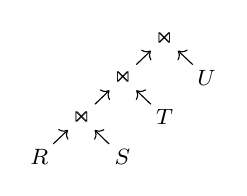
\begin{tikzpicture}[node distance=0.25cm,every node/.style={inner sep=1,outer sep=1,font=\footnotesize}]
	\node (0) {$\Join$};
	\node (1) [below left=of 0] {$\Join$};
	\node (2) [below left=of 1] {$\Join$};
	\node (R) [below left= of 2] {$R$};
	\node (S) [below right= of 2] {$S$};
	\node (T) [below right= of 1] {$T$};
	\node (U) [below right= of 0] {$U$};
    \path[->]
        (1) edge (0)
        (2) edge (1)
        (R) edge (2)
        (S) edge (2)
        (T) edge (1)
        (U) edge (0);
\end{tikzpicture}}

\newsavebox{\rightDeepTree}
\savebox{\rightDeepTree}{
	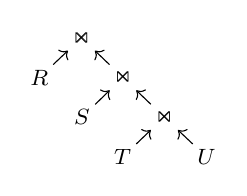
\begin{tikzpicture}[node distance=0.25cm,every node/.style={inner sep=1,outer sep=1,font=\footnotesize}]
	\node (0) {$\Join$};
	\node (1) [below right=of 0] {$\Join$};
	\node (2) [below right=of 1] {$\Join$};
	\node (R) [below left= of 0] {$R$};
	\node (S) [below left= of 1] {$S$};
	\node (T) [below left= of 2] {$T$};	
	\node (U) [below right= of 2] {$U$};
    \path[->]
        (1) edge (0)
        (2) edge (1)
        (R) edge (0)
        (S) edge (1)
        (T) edge (2)
        (U) edge (2);
\end{tikzpicture}}


\newsavebox{\bushyTree}
\savebox{\bushyTree}{
	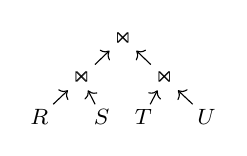
\begin{tikzpicture}[node distance=0.25cm,every node/.style={inner sep=1,outer sep=1,font=\footnotesize}]
	\node (0) {$\Join$};
	\node (1) [below left=of 0] {$\Join$};
	\node (2) [below right=of 0] {$\Join$};
	\node (R) [below left= of 1] {$R$};
	\node (S) [below right= of 1,xshift=-7.5pt] {$S$};
	\node (T) [below left= of 2,xshift=7.5pt] {$T$};	
	\node (U) [below right= of 2] {$U$};
    \path[->]
        (1) edge (0)
        (2) edge (0)
        (R) edge (1)
        (S) edge (1)
        (T) edge (2)
        (U) edge (2);
\end{tikzpicture}}

\newsavebox{\wiggleLeftTree}
\savebox{\wiggleLeftTree}{
	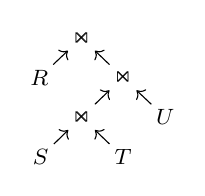
\begin{tikzpicture}[node distance=0.25cm,every node/.style={inner sep=1,outer sep=1,font=\footnotesize}]
	\node (0) {$\Join$};
	\node (1) [below right=of 0] {$\Join$};
	\node (2) [below left=of 1] {$\Join$};
	\node (R) [below left= of 0] {$R$};
	\node (S) [below left= of 2] {$S$};
	\node (T) [below right= of 2] {$T$};	
	\node (U) [below right= of 1] {$U$};
    \path[->]
        (1) edge (0)
        (2) edge (1)
        (R) edge (0)
        (S) edge (2)
        (T) edge (2)
        (U) edge (1);
\end{tikzpicture}}

\newsavebox{\wiggleRightTree}
\savebox{\wiggleRightTree}{
	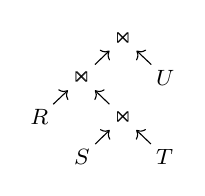
\begin{tikzpicture}[node distance=0.25cm,every node/.style={inner sep=1,outer sep=1,font=\footnotesize}]
	\node (0) {$\Join$};
	\node (1) [below left=of 0] {$\Join$};
	\node (2) [below right=of 1] {$\Join$};
	\node (R) [below left= of 1] {$R$};
	\node (S) [below left= of 2] {$S$};
	\node (T) [below right= of 2] {$T$};	
	\node (U) [below right= of 0] {$U$};
    \path[->]
        (1) edge (0)
        (2) edge (1)
        (R) edge (1)
        (S) edge (2)
        (T) edge (2)
        (U) edge (0);
\end{tikzpicture}}


%
% -----------------------------------------------------------------------------------------------
%
\begin{frame}{Query Optimization With Dynamic Programming (Sellinger, 1979)}

Dynamic programming is an algorithmic problem-solving technique suitable for optimization problems where the solution builds on solutions to sub-problems. 

\underline{Dynamic programming works bottom-up}: decompose the problem into every atomic sub-problem and solve them; the solution with $n+1$ sub-problems builds on the lowest cost solution of size $n$.

\vskip2em

\begin{center}
\begin{tikzpicture}[node distance=0.25cm,every node/.style={inner sep=1,outer sep=1,font=\footnotesize}]

\node (0) {$\pi_{a_1,\ldots,a_n}$};
\node (1) [below= of 0] {$\sigma_{c_1 \wedge c_2}$};
\node (2) [below= of 1] {$\Join$};
\node (3) [below left= of 2] {$\Join$};
\node (4) [below right= of 2] {$T$};
\node (3a) [below left= of 3] {$R$};
\node (3b) [below right= of 3] {$S$};
\path[->]
        (1) edge (0)
        (2) edge (1)
        (3) edge (2)
        (4) edge (2)
        (3a) edge (3)
        (3b) edge (3);

\node (5) [right= 1cm of 1] {$\pi_{a_1,\ldots,a_n}$};
\node (6) [right= of 5] {$\sigma_{c_1}$};
\node (7) [right= of 6] {$\sigma_{c_2}$};
\node (8) [right= of 7] {$\Join$};
\node (9) [right= of 8] {$\Join$};
\node (10) [right= of 9] {$R$};
\node (11) [right= of 10] {$S$};
\node (12) [right= of 11] {$T$};
\end{tikzpicture}
\end{center}
\end{frame}

%
% -----------------------------------------------------------------------------------------------
%
\begin{frame}{Dynamic Programming Optimizer}

\textbf{Step 1:} for each atomic sub-problem $Q$, compute:
\begin{itemize}[-,topsep=-0.5em,noitemsep]
\item $T(Q) \text{ or } B(Q)$: the estimated size of $Q$
\item $\mathit{plan}(Q)$: the lowest-cost plan to compute $Q$
\item $\alert{\mathit{cost}(Q)}$: the actual cost to compute $Q$.
\end{itemize}

\vskip1em

\textbf{Step 2:} build, recursively, all legal solutions of size $n+1$, considering all combinations of a solution of size $n$ and the solution to another sub-problem. Keep the one with least cost.

\vskip1em

Invalid partial solutions (e.g., doing a projection ``before scanning a table'') are discarded.
\end{frame}


\begin{frame}

The \alert{cost function} needs to take into account \textbf{both} \blue{I/O} \textbf{and} \blue{memory} costs. However, these two costs have different units, so we cannot just add them up.

Different systems achieve this goal differently. One simple way is to consider the number of tuples that are read and computed. 

For example:

\begin{itemize}[-,topsep=-0.5em,noitemsep]
\item $\mathit{cost}(R) = T(R)$
\item $\mathit{cost}(\rho_{S(s_1,\ldots,s_n)}(R)) = \alert{\mathit{cost}(R)}$
\item $\mathit{cost}(\sigma_C(R)) = T(\sigma_C(R)) + \alert{\mathit{cost}(R)}$
\item $\mathit{cost}(\pi_{a_1,\ldots,a_n}(R)) = T(\pi_{a_1,\ldots a_n}(R)) + \alert{\mathit{cost}(R)}$
\item $\mathit{cost}(R\Join_C S)\blue{\footnotemark} = T(R \Join_C S) + \alert{\mathit{cost}(R)+\mathit{cost}(S)}$ 
\end{itemize}

\footnotetext{This is an in-memory nested-loop-join.}
\end{frame}

% %
% % -----------------------------------------------------------------------------------------------
%
\begin{frame}{Why is Join Ordering Important?}

There is a combinatorial number of plans that join $N$ relations. 

\textbf{Example:} $N=4$. Here are the 5 ``shapes'' for a 4-way join:

\begin{center}
\begin{tikzpicture}[node distance=0.25cm]
\node (0) {\scalebox{0.75}{\usebox{\leftDeepTree}}};
\node (1) [right=of 0] {\scalebox{0.75}{\usebox{\rightDeepTree}}};
\node (2) [right=of 1] {\scalebox{0.75}{\usebox{\bushyTree}}};
\node (3) [right=of 2] {\scalebox{0.75}{\usebox{\wiggleLeftTree}}};
\node (4) [right=of 3] {\scalebox{0.75}{\usebox{\wiggleRightTree}}};
\end{tikzpicture}
\end{center}

With each shape\footnote{The number of shapes comes from \url{https://en.wikipedia.org/wiki/Catalan_number}.} we can have any of the permutations of the relations. With relations there are $4!(\frac{6!}{(4! \cdot 3!)})=120$ alternatives. 

With 5 relations, there are $5!(\frac{8!}{(5! \cdot 4!)})=1,680$ alternatives.

\end{frame}

%
% -----------------------------------------------------------------------------------------------
%
\begin{frame}
How many \textbf{actual} plans? 

The space of possible plans considers, \underline{for every single one} of the 120 ways of performing the 4-way join, \underline{all possible} \textbf{legal rewrites} of the query (i.e., pushing selections down or not?) and, for each rewrite, \underline{all possible} algorithms for each of the joins (nested-loop, hash-join, merge-join,...) and scans (table scan, index scan, if so, which one?).

Considering all these plans would almost always take longer than executing a ``reasonable'' one.

\vskip1em
\end{frame}


%
% -----------------------------------------------------------------------------------------------
%
\begin{frame}{Left Deep Plans}

\begin{columns}[onlytextwidth]
\begin{column}{0.5\textwidth}
Back to the $N=4$ case. 

\vskip1em

Among all 120 plans, only $4!=24$ are ``left-deep''
\end{column}
\begin{column}{0.3\textwidth}
{\scalebox{1}{\usebox{\leftDeepTree}}}
\end{column}
\end{columns}

\vskip1em

A ``left-deep'' binary tree is one in which all right children are leaves.

There are two main advantages of restricting the search to left-deep plans:
\begin{enumerate}[(1),topsep=-0.5em,noitemsep]
\item The search space is much smaller.
\item These plans work well in the pipeline fashion of the iterator-style query answering.
\end{enumerate}

\end{frame}

%
% -----------------------------------------------------------------------------------------------
%
\begin{frame}[fragile]
\label{worked_example}
\textbf{Worked example:} Finding the best left-deep plan based on estimated cost.

\vskip2em

\begin{columns}[onlytextwidth]
\begin{column}{0.4\textwidth}
$R(a,b,c)$ \qquad $S(c,d,e)$\\
 $T(b,f,g)$ 

\vskip2em

\begin{lstlisting}[style=SQL]
SELECT *
FROM R JOIN S 
   JOIN T JOIN  U
WHERE f > 10
\end{lstlisting}
\end{column}
\small
\begin{column}{0.6\textwidth}
\begin{tabular}{c|r|rrr}
& $T(\cdot)$ & \multicolumn{3}{c}{$V(\cdot,\cdot)$}\\
\hline
\multirow{2}{*}{$R$} & \multirow{2}{*}{10,000} & $a$ & $b$ & $c$\\
& & 500 & 1000 & 500 \\
\hline
\multirow{2}{*}{$S$} & \multirow{2}{*}{20,000} & $c$ & $d$ & $e$\\
& & 2,000 & 200 & 250 \\
\hline
\multirow{2}{*}{$T$} & \multirow{2}{*}{3,000} & $b$ & $f$ & $g$\\
& & 1,500 & 20 & 2 \\
\hline
\end{tabular}
\end{column}
\end{columns}

\vskip1em

Assume:

\begin{itemize}[-,noitemsep,topsep=-5pt]
 \item $s(f > 10, T) = 0.01$
\item $\MIN(f, T) = -20$
\item $\MAX(f, T) = 20$
\end{itemize} 

\end{frame}

\def\selectionPlan#1#2{
	\begin{tikzpicture}[node distance=0.75cm,every node/.style={inner sep=1,outer sep=1,font=\scriptsize}]
	\node (0) {#1};
	\node (1) [below of= 0] {#2};
	\path[->] (1) edge (0);
	\end{tikzpicture}
}

\def\twoRelationLDPlan#1#2{
	\begin{tikzpicture}[node distance=0.25cm,every node/.style={inner sep=1,outer sep=1,font=\scriptsize}]
	\node (0) {$\Join$};
	\node (1) [below left= of 0,xshift=5pt] {$#1$};
	\node (2) [below right= of 0,xshift=-5pt] {$#2$};
    \path[->]
        (1) edge (0)
        (2) edge (0);
	\end{tikzpicture}
}


\def\threeRelationLDPlan#1#2#3{
	\begin{tikzpicture}[node distance=0.25cm,every node/.style={inner sep=1,outer sep=1,font=\scriptsize}]
	\node (0) {$\Join$};
	\node (1) [below left= of 0,xshift=5pt] {$\Join$};
	\node (2) [below left= of 1,xshift=5pt] {$#1$};
	\node (3) [below right= of 1,xshift=-5pt] {$#2$};
	\node (4) [below right= of 0,xshift=-5pt] {$#3$};
    \path[->]
        (1) edge (0)
        (2) edge (1)
        (3) edge (1)
        (4) edge (0);
	\end{tikzpicture}
}


%
% -----------------------------------------------------------------------------------------------
%
\begin{frame}


\textbf{All} plans of size 1 (i.e., with a single node) are table scans:

\begin{tabular}{r@{\hspace*{2em}}rr}
$Q= R$ & $T(Q) = 10K$ & $\mathit{cost}(Q) = 10K$ \\
$Q= S$ & $T(Q) = 20K$ & $\mathit{cost}(Q) = 20K$ \\
$Q= T$ & $T(Q) = 3K$ & $\mathit{cost}(Q) = 3K$ \\
\end{tabular}

The nodes $\Join$, $\Join$, and $\sigma_{f>10}$ cannot be used alone and thus cannot be part of a single-node plan 


\vskip3em

There is \textbf{only one} valid plan of size 2:

\begin{tabular}{r@{\hspace*{2em}}rr}
 $Q=$ \selectionPlan{$\sigma_{f>10}$}{$T$} & $T(Q)=3K \cdot 0.01 = 30$ & $\mathit{cost}(Q) = 3.03K$
\end{tabular}

\alert{NOTE:} $V(\sigma_{f>10}(T), b) = 30$, although the original table had a lot more distinct values of $b$ (recall slide~\ref{worked_example}).

\end{frame}

\begin{frame}

Now, plans with a \textbf{single join}, starting with those of size 3:

\begin{tabular}{r@{\hspace*{2em}}rr}
 $Q=$ \twoRelationLDPlan{S}{R} & $T(Q) = \frac{10K \cdot 20K}{\max(500,2K)}=100K$ & $\mathit{cost}(Q) = 130K$ \\
 $Q=$ \twoRelationLDPlan{R}{T} & $T(Q) = \frac{10K \cdot 3K}{\max(1K,1.5K)}=20K$ & $\mathit{cost}(Q) = 33K$ \\
 $Q=$ \twoRelationLDPlan{S}{T} & $T(Q) = 20K\cdot3K =60M$ & $\mathit{cost}(Q) = 60.023M$ \\
\end{tabular}

\vskip2em

\alert{NOTE:} query plan \twoRelationLDPlan{S}{T} has a high cost because it is a \emph{cross product}: there are no attributes common to $S$ and $T$.
\begin{itemize}[-,topsep=-5pt]
\item A modern optimizer will immediately prune that sub-plan as it cannot be better than any other plan.
\end{itemize}

\end{frame}

%
% -----------------------------------------------------------------------------------------------
%

\def\joinSelectionLDplan#1{
	\begin{tikzpicture}[node distance=0.25cm,every node/.style={inner sep=1,outer sep=1,font=\scriptsize}]
	\node (0) {$\Join$};
	\node (1) [below left= of 0,xshift=5pt] {$#1$};
	\node (2) [below right= of 0,xshift=-5pt] {$\sigma_{f>10}$};
	\node (3) [below of= 2, yshift=-0.35cm] {$T$};
    \path[->]
        (1) edge (0)
        (2) edge (0)
        (3) edge (2);
	\end{tikzpicture}
}

\def\selectionJoinLDplan#1{
	\begin{tikzpicture}[node distance=0.25cm,every node/.style={inner sep=1,outer sep=1,font=\scriptsize}]
	\node (0) {$\sigma_{f>10}$};
	\node (1) [below of= 0, yshift=-0.35cm] {$\Join$};
	\node (2) [below left= of 1,xshift=5pt] {$#1$};
	\node (3) [below right= of 1,xshift=-5pt] {$T$};
    \path[->]
        (1) edge (0)
        (2) edge (1)
        (3) edge (1);
	\end{tikzpicture}
}


\begin{frame}

Now, plans of size 4 (single-join with $T$ and $\sigma_{f>10}$).

We will ignore the plans involving the cross product $S\Join T$, and consider the only two plans involving $R$ and $T$:

\vskip2em


\begin{columns}[onlytextwidth]
\begin{column}{0.3\textwidth}
$Q = $ \joinSelectionLDplan{R}
\end{column}
\begin{column}{0.3\textwidth}
\begin{align*}
T(Q) = \frac{10K\cdot 30}{\max(1K,30)} = 300\\
\mathit{cost}(Q) = 300 + 10K + 3.03K = \alert{13.33K}
\end{align*}
\end{column}
\end{columns}

\vskip2em

For the next one, we re-use the work done for plans of size 3.

\begin{columns}[onlytextwidth]
\begin{column}{0.3\textwidth}
$Q = $ \selectionJoinLDplan{R}
\end{column}
\begin{column}{0.3\textwidth}
\begin{align*}
T(Q) = 20K\cdot 0.01 = 200\\
\mathit{cost}(Q) = 200 + 33K = 33.2K
\end{align*}
\end{column}
\end{columns}


\end{frame}


%
% -----------------------------------------------------------------------------------------------
%
\begin{frame}

\vskip1em

Now for plans of size 5, which would be the best plans of size 3 plus another join (and another table).

\vskip1em

\begin{columns}[onlytextwidth]
\begin{column}{0.3\textwidth}
$Q = $ \threeRelationLDPlan{S}{R}{T} 
\end{column}
\begin{column}{0.3\textwidth}
\begin{align*}
 T(Q) &= \frac{T(R,S,\Join)T(T)}{\max(V(b,R\Join S),V(b,T))}\\
&=\frac{100K\cdot 3K}{\max(1K, 1.5K)}=200K\\
\mathit{cost(Q)} &= 200K + 130K + 3K = 363K
\end{align*}
\end{column}
\end{columns}

\vskip2em

\begin{columns}[onlytextwidth]
\begin{column}{0.3\textwidth}
$Q = $ \threeRelationLDPlan{R}{T}{S} 
\end{column}
\begin{column}{0.3\textwidth}
\begin{align*}
T(Q) &= \frac{20K \cdot 20K}{\max(500,2K)} =200K\\
\mathit{cost(Q)} &= 200K + 33K + 20K = \alert{253K}
\end{align*}
\end{column}
\end{columns}


\vskip2em

Again, we ignore the plan with $S\Join T$.


\end{frame}

%
% -----------------------------------------------------------------------------------------------
%


\begin{frame}

An now for plans of size 6, that will include all nodes.


\vskip1em

\textbf{Option 1:} add $\sigma_{f>10}$ to the \textbf{best} plan of size 5.

\vskip1em

\begin{columns}[onlytextwidth]
\begin{column}{0.3\textwidth}
$Q = $ 	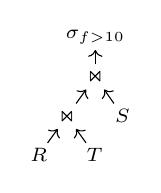
\begin{tikzpicture}[node distance=0.25cm,every node/.style={inner sep=1,outer sep=1,font=\scriptsize}]
	\node (s) {$\sigma_{f>10}$};
	\node (0) [below of=s, yshift=-0.25cm] {$\Join$};
	\node (1) [below left= of 0,xshift=5pt] {$\Join$};
	\node (2) [below left= of 1,xshift=5pt] {$R$};
	\node (3) [below right= of 1,xshift=-5pt] {$T$};
	\node (4) [below right= of 0,xshift=-5pt] {$S$};
    \path[->]
        (0) edge (s)
        (1) edge (0)
        (2) edge (1)
        (3) edge (1)
        (4) edge (0);
	\end{tikzpicture}
\end{column}

\begin{column}{0.5\textwidth}
\begin{align*}
T(Q) & = 200K \cdot 0.01 = 20K\\
\mathit{cost}{Q} & = 20K + 253K = 273K
\end{align*}
\end{column}
\end{columns}


\vskip2em

\textbf{Option 2:} join $S$ to the \textbf{best} plan of size 4.

\vskip1em

\begin{columns}[onlytextwidth]
\begin{column}{0.3\textwidth}
$Q = $ 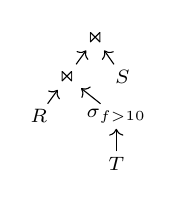
\begin{tikzpicture}[node distance=0.25cm,every node/.style={inner sep=1,outer sep=1,font=\scriptsize}]
	\node (j) {$\Join$};
	\node (0) [below left= of j,xshift=5pt]{$\Join$};
	\node (5) [below right= of j,xshift=-5pt] {$S$};
	\node (1) [below left= of 0,xshift=5pt] {$R$};
	\node (2) [below right= of 0,xshift=-5pt] {$\sigma_{f>10}$};
	\node (3) [below of= 2, yshift=-0.35cm] {$T$};
    \path[->]
        (0) edge (j)
        (5) edge (j)
        (1) edge (0)
        (2) edge (0)
        (3) edge (2);
	\end{tikzpicture}
\end{column}

\begin{column}{0.5\textwidth}
\begin{align*}
T(Q) & = \frac{300\cdot 20K}{\max(500,2K)} = 3K\\
\mathit{cost}{Q} & = 3K + 13.33K + 20K = \alert{36.33K}
\end{align*}
\end{column}
\end{columns}

\vskip1em

\blue{And we are done!}
\end{frame}

%
% -----------------------------------------------------------------------------------------------
%
\begin{frame}{Notes}

The Sellinger optimizer can handle all operators in a SQL query, choosing the best place for each operator.

\begin{enumerate}[(1)]
\item Note that it ``figured out'' that pushing selections down the tree is the right thing to do. Although we would save more time by always pruning plans with ``high'' selections.

\item However, even with aggressive pruning, Dynamic programming is too expensive to be practical.
\begin{itemize}[-,noitemsep,topsep=-5pt]

\item Commercial optimizers often use many heuristics and avoid enumerating all plans as we did here. 
\end{itemize}

\item Machine learning can help by providing better cost estimates and also by helping solve the optimization problem.

\end{enumerate}
\end{frame}


%%%%%%%%%%%%%%%% ------------------------

\section{Query Plans with Indexes}
%!TEX root = lec05_query_processing.tex


\begin{frame}

Recall that indexes as \emph{associative access methods} that allow the DBMS to quickly find tuples based on the values of their attributes.

B+ tree indexes, hash tables and hash sets can be used to implement many query plan operators: selections, joins (and their variants), all set operators, duplicate elimination, and grouping.

The next slides give some examples of the use of indexes.

We start by looking at \textbf{base indexes}, or indexes created by the database administrator, and discuss briefly the idea of on-the-fly indexing, which is to create an index with the result of a sub-query to be used once.

\end{frame}

\begin{frame}[fragile]

\vskip1em
The table below indicates, generally, which kinds of predicates can be improved by the use of \textbf{indexes}.

\vskip1.5em

\begin{center}
\begin{tabular}{l||c|c|c||c|c}
\hline
& $a_i = v$ & $a_i \geq v$ & $a_i$ \texttt{\footnotesize IN ()} & $a_i \neq v$ &  $a_i$ \texttt{\footnotesize NOT IN ()}\\
\hline\hline
B+ tree & \cmark & \cmark$^\dagger$ & \cmark & \xmark$^\ddagger$ & \cmark\\
Hash table & \cmark & \xmark & \cmark & \xmark$^\ddagger$ & \cmark\\
\hline
\end{tabular}
\end{center}

\vskip1em

\footnotesize

$^\dagger$ If the B+tree is a secondary index and the selectivity of the predicate is high, a table scan might be better.

$^\ddagger$ These predicates often \alert{have very high selectivity}, so the table scan is \alert{almost always better}.

\normalsize
\end{frame}

%
% -----------------------------------------------------------------------
%

\newsavebox{\PickingIndexesExample}
\begin{lrbox}{\PickingIndexesExample}
\begin{lstlisting}[style=SQL]
SELECT director
FROM Movie
WHERE title='Ghostbusters' AND year=1984
\end{lstlisting}
\end{lrbox}

\begin{frame}[fragile]{How are Indexes Chosen?}

A predicate \alert{\lstinline[mathescape]!$a_i\ $<op>$\ v$!} in the \lstinline[style=SQL]{WHERE} clause can be answered using an index only if \alert{$a_i$ is a prefix of the index key}.

\vskip1em

\textbf{Example:}\qquad \framebox{\scalebox{0.8}{\usebox\PickingIndexesExample}}

\vskip1em

\begin{columns}[onlytextwidth]
\begin{column}{0.45\textwidth}
\begin{block}{Useful Indexes}
\lstinline[style=SQL]{Movie(title)}, ~~~~ \lstinline[style=SQL]{Movie(year)},\\
\lstinline[style=SQL]{Movie(title,imdb)}, ... 
\end{block}
\end{column}
\begin{column}{0.45\textwidth}
\begin{block}{Not Useful}
\lstinline[style=SQL]{Movie(imdb,title)}, \\
\lstinline[style=SQL]{Movie(director)} ... 
\end{block}
\end{column}
\end{columns}

\vskip1em
If multiple useful indexes exist, the DBMS picks the one with lowest estimated cost, which depends on the selectivity of the predicate!
\end{frame}


%
% -----------------------------------------------------------------------
%
\begin{frame}[fragile]

\begin{center}
\small
\begin{tabular}{r|l}
$T(\text{Movie}) = 100,000$ & $V(\text{Movie}, \text{title}) = 95,000$ \\
$S(\text{Movie}) = 92$ & $V(\text{Movie}, \text{year}) = 32$ \\
$B(\text{Movie}) = 2,000$ & $V(\text{Movie}, \text{imdb}) = 50$ \\
 & $V(\text{Movie}, \text{director}) = 25,000$ \\
\end{tabular}
\normalsize
\end{center}

\vskip2em

Suppose we have the following B+ tree indexes with 100 pointers/node.

\vskip1em

\begin{quote}
\lstinline[style=SQL]{> CREATE INDEX IDX1 ON Movie(Title);}
\lstinline[style=SQL]{> CREATE INDEX IDX2 ON Movie(Title,Year);}
\lstinline[style=SQL]{> CREATE INDEX IDX3 ON Movie(Year);}
\end{quote}

In all cases, 3 levels are enough to index all keys.

\end{frame}


\begin{frame}[fragile]

How many blocks (at the leaf level) of each index will have tuples matching the query?

\small
\[T(\sigma_{\texttt{title='Ghostbusters'}}(\texttt{Movie})) = \ceil*{\frac{100,000}{95,000}}=2\]
\[T(\sigma_{\texttt{year=1984}}(\texttt{Movie})) = \ceil*{\frac{100,000}{32}}=3,125\]
\normalsize

\vskip1em

\begin{block}{\alert{We can thus expect to find:}}
 - all movies with that title in a single \textbf{leaf} block of \lstinline[style=SQL]{IDX1}\\
 - all movies from 1984 in 32 \textbf{leaf} blocks of \lstinline[style=SQL]{IDX3}\\
 - all movies with that title/year in a single \textbf{leaf} block of \lstinline[style=SQL]{IDX2}
\end{block}
\end{frame}

%
% -----------------------------------------------------------------------
%
\begin{frame}[fragile]

\begin{center}
\framebox{\scalebox{0.8}{\usebox\PickingIndexesExample}}
\end{center}

\vskip2em

\begin{columns}
\begin{column}{0.125\textwidth}
\begin{tikzpicture}[semithick,align=center,node distance=0.75cm,every node/.style={inner sep=1,outer sep=1,font=\footnotesize}]
\node (0) at (0,0) {} ; %empty node with ``answer''
\node (1) [below of= 0] {$\pi_{\texttt{director}}$};
\node (2) [below of= 1] {$\sigma_{\substack{\texttt{title='Ghostbusters'}\\\wedge\, \texttt{year=1984}}}$};
\node (3) [below of= 2] {\lstinline[style=SQL]{scan(Movie)}};
\path[->]
    (3) edge (2)
    (2) edge (1)
    (1) edge (0);
\end{tikzpicture}
\end{column}
\begin{column}{0.5\textwidth}
\begin{center}
\begin{tikzpicture}[semithick,align=center,node distance=0.8cm,every node/.style={inner sep=1,outer sep=1,font=\footnotesize}]
\node (0) at (0,0) {} ; %empty node with ``answer''
\node (1) [below of= 0] {$\pi_{\texttt{director}}$};
\node (2) [below of= 1] {$\sigma_{\texttt{year=1984}}$};
\node (3) [below of= 2] {\lstinline[style=SQL]{pointer_lookup}};
\node (4) [below of= 3] {\lstinline[style=SQL]{search(IDX1, =, "Ghostbusters")}};
\path[->]
    (4) edge (3)
    (3) edge (2)
    (2) edge (1)
    (1) edge (0);

\pause
\node (5) [node distance=2.5cm,left of=2,color=blue] {\begin{minipage}{2.15cm}\baselineskip=0.75\baselineskip \centering
follow the pointer to get the entire tuple 
\end{minipage}};
\draw [color=blue,->] (5) -- (3);
\end{tikzpicture}
\end{center}
\end{column}
\end{columns}

\vskip1em

\begin{block}{\alert{Estimated I/O costs:}}
 - left plan: 2,000 blocks\\
 - right plan: 3 \textcolor{blue}{+ 2} = \alert{5} blocks\footnotemark
\end{block}

\footnotetext{3 I/Os on the index (root to leaf path) + 2 lookups on the table.}

\end{frame}

%
% -----------------------------------------------------------------------
%

\begin{frame}{Cost recap}

The cost of retrieving tuples from a table $R$ satisfying a predicate $p$ using a a \alert{B+ Tree} with $|I|$ blocks at the \emph{leaf level} is the sum of:

\begin{enumerate}[(1),noitemsep]
\item Number of inner blocks in the path from root to the first index leaf (usually 2 or 3).
\item Number of blocks of the index that will be read: \(\ceil*{s(p) \cdot |I|}\). 
\item Number of pointer lookups: \(T(\sigma_p (R))\) (unless this is a primary index and the table is sorted as the index).
\end{enumerate}

\vskip1em

With a \alert{hash table}, the estimated cost is \(T(\sigma_p (R)) \cdot 2\): one read in the hash table and another for the pointer traversal to the table.

\end{frame}


%
% -----------------------------------------------------------------------
%
\begin{frame}[fragile]{Covering Index}

The \alert{\lstinline[style=SQL]{pointer_lookup}} operator pulls a pointer to a tuple in \lstinline[style=SQL]{Movie} returned by the index search operator and goes to the block of file of the \lstinline[style=SQL]{Movie} table that contains the respective tuple and fetches it.

This operator is needed because the query uses attributes of \lstinline[style=SQL]{Movie} that are not present in the index record (\lstinline[style=SQL]{year} and \lstinline[style=SQL]{director}).

\vskip1em

\begin{columns}[onlytextwidth]
\begin{column}{0.45\textwidth}
An index with all attributes from the table used in a query is called a \alert{covering index}.
\end{column}

\begin{column}{0.5\textwidth}
\begin{lstlisting}[style=SQL]
SELECT year
FROM Movie
WHERE title='Ghostbusters'
\end{lstlisting}
\end{column}
\end{columns}

\lstinline[style=SQL]{IDX2} is a covering index for the query above.

\end{frame}

%
% -----------------------------------------------------------------------
%
\begin{frame}[fragile]{Index-Based Joins}

Depending on whether the index is primary or not, and on the selectivity of a join predicate, the DBMS might use a base index to speed up a nested-loop join:

% \vskip1em

\begin{columns}[onlytextwidth]
\begin{column}{0.35\textwidth}
\begin{lstlisting}[style=SQL,basicstyle=\scriptsize\ttfamily]
SELECT role, imdb
FROM Movie 
  JOIN Cast 
WHERE actor='Bill Murray';
\end{lstlisting}
\end{column}
\begin{column}{0.6\textwidth}
\begin{center}
\vspace*{-2em}
\scalebox{0.85}{
    \begin{tikzpicture}[semithick,align=center,node distance=0.875cm,every node/.style={inner sep=1,outer sep=1,font=\footnotesize}]
\node (0) at (0,0) {} ; %empty node with ``answer''
\node (1) [below of= 0] {$\pi_{\texttt{role,imdb}}$};

\node (2) [below of= 1] {$\Join$};
\node (3) [below right= of 2] {\lstinline[style=SQL]{pointer_lookup}} ;
\node (4) [below left= of 2] {$\sigma_{\texttt{actor='Bill Murray'}}$};
\node (5) [below of= 3] {\lstinline[style=SQL,mathescape]!search(IDX2, =, (t.title, t.year))!};
\node (6) [below of =4] {\lstinline[style=SQL]{scan(Cast)}};

\draw[->,color=accent,thick,densely dotted] (2) to[out=270,in=135] (5.north west);

\path[commutative diagrams/.cd, every arrow, every label]
    (6) edge (4)
    (4) edge node {$t$} (2) 
    (5) edge (3)
    (3) edge (2)
    (2) edge (1)
    (1) edge (0);
\end{tikzpicture}
}
\end{center}
\end{column}
\end{columns}

\vskip1em

The I/O cost is bound by $s(\text{Cast},\text{actor='Bill Murray'})$.

Of course, if there was an index on \lstinline[style=SQL]{Cast(actor)}, it could also be used instead of the table scan in the example above.

\end{frame}

\begin{frame}[fragile]{On the Fly Indexing}

\vskip2em

\begin{columns}[onlytextwidth]
\begin{column}{0.45\textwidth}

The DBMS might create an index/hash table/hash set with the results of a sub-query to speed up a join.

\vskip1em

\begin{lstlisting}[style=SQL,basicstyle=\scriptsize\ttfamily]
SELECT actor, role
FROM Cast
WHERE (title,year) IN (
    SELECT film, year
    FROM Guide
    WHERE theater='Garneau');
\end{lstlisting}
\end{column}
\begin{column}{0.5\textwidth}
\begin{center}
\vspace*{-2em}
\scalebox{0.85}{
    \begin{tikzpicture}[semithick,align=center,node distance=0.875cm,every node/.style={inner sep=1,outer sep=1,font=\footnotesize}]
\node (0) at (0,0) {} ; %empty node with ``answer''
\node (1) [below of= 0] {$\pi_{\texttt{actor,role}}$};
\node (2) [below of= 1] {\alert{$\ltimes$}};
\node (3) [below left= of 2] {\lstinline[style=SQL]{scan(Cast)}}; 
\node (4) [below right= of 2] {\lstinline[style=SQL]{create_hash_set()}} ;
\node (5) [below of= 4] {$\pi_{\texttt{film,year}}$};
\node (6) [below of= 5] {$\sigma_{\texttt{theater}=\text{``Garneau''}}$};
\node (7) [below of= 6] {\lstinline[style=SQL]{scan(Guide)}};

\path[->]
    (7) edge (6)
    (6) edge (5)
    (5) edge (4)
    (4) edge (2) 
    (3) edge (2)
    (2) edge (1)
    (1) edge (0);
\end{tikzpicture}
}
\end{center}
\end{column}
\end{columns}

\vskip1em

Recall the \textbf{semijoin} \alert{$R \ltimes S$} returns tuples from $R$ that match a tuple in $S$ with respect to the join attributes (\lstinline[style=SQL]{title,year}).

\end{frame}


\begin{frame}[fragile]{Answering Complex Predicates with Secondary Indexes}

Primary indexes allow the fastest access to tuples in the corresponding table because \alert{the tuples in the table file are sorted in the same way as the keys in the index}.\\
 - these indexes are sometimes called \textbf{clustered indexes}

\vskip1em

The problem is there can be only one primary index per table.

\vskip1em

A way to bring some of the benefits of primary to secondary indexes is to \textbf{cluster tuple identifiers} based on search key in an a ``bucket file'' and have a primary index over that file.

\end{frame}


%
% Key-pointer measurements
%
\newlength{\indexKeyBoxWidth}
\setlength{\indexKeyBoxWidth}{\dimexpr 2em\relax}

\newlength{\pointerBoxWidth}
\setlength{\pointerBoxWidth}{\dimexpr 2.5em\relax}

%
% Tuple measurements
%
\newlength{\tupleHeight}
\setlength{\tupleHeight}{\dimexpr 1.1em\relax}

\newlength{\dummyTupleGreyBoxWidth}
\setlength{\dummyTupleGreyBoxWidth}{\dimexpr 5em\relax}

%
% Data Block measurements
%

\newlength{\tupleWidth}
\setlength{\tupleWidth}{\dimexpr(\indexKeyBoxWidth+\dummyTupleGreyBoxWidth)\relax}

\newlength{\dataBlockWidth}
\setlength{\dataBlockWidth}{\dimexpr(\tupleWidth+1pt)\relax}

\def\tuplesPerDataBlock{2}

\newlength{\dataBlockHeight}
\setlength{\dataBlockHeight}{\dimexpr1pt+(\tupleHeight+0.5pt)*\the\numexpr\tuplesPerDataBlock\relax}

%
% Index block measurements
%
\newlength{\indexBlockWidth}
\setlength{\indexBlockWidth}{\dimexpr(\indexKeyBoxWidth+\pointerBoxWidth+1pt)\relax}

\def\keyPointerPairsPerIndexBlock{4}

\newlength{\indexBlockHeight}
\setlength{\indexBlockHeight}{\dimexpr1pt+(\tupleHeight+0.5pt)*\the\numexpr\keyPointerPairsPerIndexBlock\relax}

\newlength{\indexBlockPointerOffset}
\setlength{\indexBlockPointerOffset}{\dimexpr(\indexBlockHeight-1em-1pt)\relax}


\tikzset{ % same as tuple, except for the anchor part
	indexKeyBox/.style={
		draw,rectangle,minimum width=\indexKeyBoxWidth,minimum height=\tupleHeight,inner sep=0,outer sep=0,font=\footnotesize
	}
}

\tikzset{
	tupleGrayBox/.style={
		draw, rectangle, minimum width=\dummyTupleGreyBoxWidth,minimum height=\tupleHeight,outer sep=0,fill=tupleBoxColor
	}
}

% #1 --> block id
% #2,#3 --> data block id and order inside block
% #4 --> key
\def\tuple#1#2#3#4{
  \node ({#1}) at ([xshift=1pt,yshift=\dimexpr -1pt-(\tupleHeight+0.5pt)*#3]{#2}.north west) [anchor=north west,indexKeyBox] {{#4}};
  \node [right = -0.5pt of {#1}] [tupleGrayBox] {};
}


% #1 --> block id
% #2,#3 --> data block id and order inside block
% #4 --> key
\def\tupleFromBox#1#2#3#4{
  \node ({#1}) at ([xshift=1pt,yshift=\dimexpr -1pt-(\tupleHeight+0.5pt)*#3]{#2}.north west) [anchor=north west,indexKeyBox] {{#4}};
}


% --------------------------------- index key-pointer tuples

\tikzset{
	keyPointerValue/.style={
		anchor=north west,
		draw,rectangle,minimum width=\indexKeyBoxWidth,minimum height=\tupleHeight,inner sep=0,outer sep=0,font=\footnotesize
	}
}

\tikzset{ 
	keyPointerPointerBox/.style={
		draw, rectangle, minimum width=\pointerBoxWidth,minimum height=\tupleHeight,outer sep=0,fill=snow
	}
}


% #1     --> id of key-pointer (i.e., the node with the value)
% #2, #3 --> id of indexBlock and ordinal within block
% #4     --> value in the attribute of the tuple
\def\keyPointer#1#2#3#4{
  \node ({#1}) at ([xshift=1pt,yshift=\dimexpr -1pt-(\tupleHeight+0.5pt)*#3]{#2}.north west) [anchor=north west,indexKeyBox] {{#4}};
  \node [right = -0.5pt of {#1}] [keyPointerPointerBox] {};
}


% --------------------------------- blocks of the data file

\tikzset{
	dataBlockBox/.style={
		xshift=-0.1em,yshift=0.1em,anchor=north west,draw,rectangle,minimum width=\dataBlockWidth,minimum height=\dataBlockHeight
	}
}

\tikzset{
	dataBlockPointerBox/.style={
		yshift=0.125pt,
		outer sep=0,anchor=south west, draw, rectangle, 
		minimum width=1em, minimum height=1em,fill=snow
	}
}

% #1     --> block id
% #2, #3 --> block top-left coordinates
\def\dataBlock#1#2#3{
	\node ({#1}) at ({#2},{#3}) [dataBlockBox] {};
	\node at ({#1}.south east) [dataBlockPointerBox] {};
}

% #1     --> block id
% #2     --> id of block ``below'' #1
\def\linkDataBlocks#1#2{
	\draw [*->,>=stealth'] ([xshift=5pt,yshift=7pt]{#1}.south east) to[out=270,in=90] ([xshift=-10pt]#2.north east);
}

% --------------------------------- blocks of the index file


\tikzset{
	indexBlockBox/.style={
		xshift=-0.1em,yshift=0.1em,anchor=north west,draw,rectangle,minimum width=\indexBlockWidth,minimum height=\indexBlockHeight
	}
}

\tikzset{
	indexBlockPointerBox/.style={
		xshift=0.375pt,
		anchor=south east, draw, rectangle, minimum width=1em, minimum height=1em,fill=snow
	}
}

% #1     --> block id
% #2, #3 --> block top-left coordinates
% #4     --> id of the first key-pointer inside the block
% #5     --> value of the first key
\def\indexBlock#1#2#3{
	\node ({#1}) at ({#2},{#3}) [indexBlockBox] {};
	\node at ({#1}.south west) [indexBlockPointerBox] {};
}

% #1     --> block id
% #2     --> id of block ``below'' #1
\def\linkIndexBlocks#1#2{
	\draw [*->,>=stealth'] ([xshift=-5pt,yshift=7pt]{#1}.south west) to[out=270,in=90] ([xshift=10pt]#2.north west);
}

% #1 --> key-pointer id
% #2 --> tuple id
\def\KPtoTuple#1#2{
	\draw [*->,>=stealth'] ([xshift=30pt,yshift=0em]{#1}.west) to[out=0,in=180] (#2.west);
}




%%%%% MACROS FOR SPARSE INDEX WITH POINTERS TO BLOCKS

\tikzset{ 
	sparseKeyPointerPointerBox/.style={
		draw, rectangle, minimum width=1.1em,minimum height=\tupleHeight, fill=snow
	}
}

% draws two rectangles, one with an attribute value, the other with the pointer
%
% #1     --> id of key-pointer (i.e., the node with the value)
% #2, #3 --> coordinages of top-left corner of node with tuple value
% #4     --> value in the attribute of the tuple
\def\sparseKeyPointer#1#2#3#4{
  \node ({#1}) at ({#2},{#3}) [keyPointerValue] {\tiny{#4}} ;
  \node [right = -0.5pt of {#1}] [sparseKeyPointerPointerBox] {};
}

\tikzset{
	sparseIndexBlockBox/.style={
		xshift=-0.1em,yshift=0.1em,anchor=north west,draw,rectangle,minimum width=3.3em,minimum height=4.6em
	}
}

% #1     --> block id
% #2, #3 --> block top-left coordinates
% #4     --> id of the first key-pointer inside the block
% #5     --> value of the first key
\def\sparseIndexBlock#1#2#3#4#5{
	\node ({#1}) at ({#2},{#3}) [sparseIndexBlockBox] {};
	\node at ({#2},{#3}) [indexBlockPointerBox] {};
	\sparseKeyPointer{{#4}}{{#2}}{{#3}}{{#5}};
}

% #1     --> block id
% #2     --> id of block ``above'' this one
% #3, #4 --> coordinates of this block
% #5     --> id of the first tuple inside the block
% #6     --> value of the first tuple
\def\sparseIndexBlockBelow#1#2#3#4#5#6{
	\node ({#1}) at ({#3},{#4}) [sparseIndexBlockBox] {};
	\node at ({#3},{#4}) [indexBlockPointerBox] {};
	\sparseKeyPointer{{#5}}{{#3}}{{#4}}{{#6}};
	\draw [*->,>=stealth'] ([xshift=-5pt,yshift=7pt]{#2}.south west) to[out=270,in=90] ([xshift=10pt]#1.north west);
}

% #1 --> key-pointer id
% #2 --> tuple id
\def\sparseKPtoTuple#1#2{
	\draw [*->,>=stealth'] ([xshift=22.5pt,yshift=0em]{#1}.west) to[out=0,in=180] (#2.west);
}



%================================ illustration of multilevel indexes

\def\denseIndexMultilevel#1#2#3#4{
    \node ({#1}) at ({#2},{#3}) [font=\footnotesize,draw,fill=accent!25,rectangle,minimum width=2.5em,minimum height=1em] {{#4}};
    \node (t) [below = 1em of {#1}] [rectangle,minimum width=2.5em] {};
    \draw [->,>=stealth'] ({#1}) -- (t);
    \draw [->,>=stealth'] ([xshift=-2pt]{#1}.south) -- ([xshift=-6pt]t.north);
    \draw [->,>=stealth'] ([xshift=2pt]{#1}.south) -- ([xshift=6pt]t.north);
    \draw [->,>=stealth'] ([xshift=-6pt]{#1}.south) -- (t.north west);
    \draw [->,>=stealth'] ([xshift=6pt]{#1}.south) -- (t.north east);
}

\def\denseIndexMultilevelAfter#1#2#3{
    \node ({#1}) [right of= {#2}] [font=\footnotesize,draw,fill=accent!25,rectangle,minimum width=2.5em,minimum height=1em] {{#3}};
        \node (t) [below = 1em of {#1}] [rectangle,minimum width=2.5em] {};
    \draw [->,>=stealth'] ({#1}) -- (t);
    \draw [->,>=stealth'] ([xshift=-2pt]{#1}.south) -- ([xshift=-6pt]t.north);
    \draw [->,>=stealth'] ([xshift=2pt]{#1}.south) -- ([xshift=6pt]t.north);
    \draw [->,>=stealth'] ([xshift=-6pt]{#1}.south) -- (t.north west);
    \draw [->,>=stealth'] ([xshift=6pt]{#1}.south) -- (t.north east);
}


\newsavebox\genericDenseIndexWithNblocks
\savebox{\genericDenseIndexWithNblocks}{
\begin{tikzpicture}[
	every node/.append style={node distance=4em},
	every edge/.append style={>=stealth'}]
\node at (-1.5,0) [color=accent,font=\footnotesize] {Index:};

\denseIndexMultilevel{0}{0}{0}{$b_0$};
\denseIndexMultilevelAfter{1}{0}{$b_1$};
\denseIndexMultilevelAfter{2}{1}{$b_2$};
\node (3) [right of=2] {...};
\denseIndexMultilevelAfter{4}{3}{$b_{N-1}$};
\denseIndexMultilevelAfter{5}{4}{$b_{N}$};

\path [->] (0) edge (1) 
   (1) edge (2)
   (2) edge (3)
   (3) edge (4)
   (4) edge (5);
\end{tikzpicture}
}

\newsavebox\genericMultilevelIndexSparseOnDense
\savebox{\genericMultilevelIndexSparseOnDense}{
\begin{tikzpicture}[
	every node/.append style={node distance=4em},
	every edge/.append style={>=stealth'}]
\tikzset{
    block/.style={font=\footnotesize,draw,fill=snow,rectangle,minimum width=2.5em,minimum height=1em}
    }
\tikzset{
    sparseBlock/.style={font=\footnotesize,draw,fill=snow,rectangle,minimum width=2.5em,minimum height=1em}
    }

\node at (-1.5,0) [color=accent,font=\footnotesize] {\begin{minipage}{1cm}\baselineskip=0.75\baselineskip \centering
Dense Index: \end{minipage}};

\denseIndexMultilevel{0}{0}{0}{$b_0$};
\denseIndexMultilevelAfter{1}{0}{$b_1$};
\denseIndexMultilevelAfter{2}{1}{$b_2$};
\node (3) [right of=2] {...};
\denseIndexMultilevelAfter{4}{3}{$b_{N-1}$};
\denseIndexMultilevelAfter{5}{4}{$b_{N}$};

\path [->] (0) edge (1) 
   (1) edge (2)
   (2) edge (3)
   (3) edge (4)
   (4) edge (5);

\node at (-1.5,1.5) [color=accent,font=\footnotesize] {\begin{minipage}{1cm}\baselineskip=0.75\baselineskip \centering
Sparse Index: \end{minipage}};

\node [sparseBlock] (6) [xshift=1em,above of=1] {$\mathit{b}_0$};
\node (7) [xshift=1em,right of=6] {...};
\node [sparseBlock] (8) [xshift=1em,right of=7] {$\mathit{b}_M$};

\path [->] (6) edge (7)
    (7) edge (8);

\draw [->,>=stealth'] ([xshift=-9pt]6.south) to[out=270,in=90] ([xshift=2pt]0.north west);
\draw [->,>=stealth'] ([xshift=-5pt]6.south) to[out=270,in=90] ([xshift=2pt]1.north west);
\draw [->,>=stealth'] ([xshift=-1pt]6.south) to[out=270,in=90] ([xshift=2pt]2.north west);
\draw [->,>=stealth'] ([xshift=5pt]8.south) to[out=270,in=90] ([xshift=2pt]4.north west);
\draw [->,>=stealth'] ([xshift=9pt]8.south) to[out=270,in=90] ([xshift=2pt]5.north west);

\node (inv1) [xshift=2em,yshift=-1em,above right of=1,rectangle]  {...};
\draw [->,>=stealth'] ([xshift=2pt]6.south) -- (inv1.north west);
\draw [->,>=stealth'] ([xshift=9pt]6.south) -- (inv1.north east);

\node (inv2) [xshift=-2em,yshift=-1em,above right of=3,rectangle]  {...};
\draw [->,>=stealth'] ([xshift=-4pt]8.south) -- (inv2.north east);
\draw [->,>=stealth'] ([xshift=-8pt]8.south) -- (inv2.north west);
\end{tikzpicture}
}


%
% illustration scanning cost of range selection on dense primary index
%

\newsavebox{\rangeSelectionQueryPrimaryIndex}
\savebox{\rangeSelectionQueryPrimaryIndex}{
\begin{tikzpicture}
%index blocks
\node (0) at (0,0) [draw,rectangle,fill=gray!35,minimum width=1.75em,minimum height=1em] {};
\node (1) at (1,0) [rectangle,minimum width=1em,minimum height=1em] {...};
\foreach \i in {2,...,4}{
  \node (\i) at (\i,0) [draw,rectangle,fill=gray!35,minimum width=1.75em,minimum height=1em] {};  
}
\node (5) at (5,0) [rectangle,minimum width=1em,minimum height=1em] {...};    
\node (6) at (6,0) [draw,rectangle,minimum width=1.75em,minimum height=1em] {};
%chain of index blocks
\foreach \i in {1,...,6}{
    {\pgfmathsetmacro{\j}{\i - 1}
    \draw [->,>=stealth'] ({\j}) -- (\i);}
}

%data blocks
\node (7) at (0,-1) [draw,rectangle,minimum width=1.75em,minimum height=1em] {};
\node (8) at (1,-1) [rectangle,minimum width=1em,minimum height=1em] {...};
\foreach \i in {9,...,10}{
  \pgfmathsetmacro{\j}{\i - 7}
  \node (\i) at (\j,-1) [draw,rectangle,minimum width=1.75em,minimum height=1em] {};  
}
\node (11) at (4,-1) [draw,rectangle,fill=gray!35,minimum width=1.75em,minimum height=1em] {};
\node (12) at (5,-1) [rectangle,minimum width=1em,minimum height=1em] {...};    
\node (13) at (6,-1) [draw,rectangle,fill=gray!35,minimum width=1.75em,minimum height=1em] {};
%chain of data blocks
\foreach \i in {8,...,13}{
    {\pgfmathsetmacro{\j}{\i - 1}
    \draw [->,>=stealth'] ({\j}) -- (\i);}
}

%index and tuple keys
\node (k) at (3.85,0) [inner sep=0,outer sep=0,draw,fill=accent,rectangle,minimum width=0.25em,minimum height=1em] {};
\node (t) at (4.15,-1) [inner sep=0,outer sep=0,draw,fill=accent,rectangle,minimum width=0.25em,minimum height=1em] {};

%labels
\node (i) [outer sep=0pt,above left of=k,draw,color=accent] {\scriptsize $\min (x') > x$};
\node at (6.5,-1) [anchor= west]{\scriptsize Data: $N$ blocks}; 
\node at (6.5,0) [anchor= west]{\scriptsize Index: $M$ blocks}; 

\draw [color=accent,->] (i.south) to[out=270,in=90] (k.north);
\draw [->,>=stealth'] (k.south) to[out=270,in=90] (t.north);
\end{tikzpicture}
}


%
%
% --------------------------------------------------------------
%
%


\newsavebox{\rangeSelectionQueryStackedIndex}
\savebox{\rangeSelectionQueryStackedIndex}{
\begin{tikzpicture}
%index blocks
\node (0) at (0,0) [draw,rectangle,,minimum width=1.75em,minimum height=1em] {};
\node (1) at (1,0) [rectangle,minimum width=1em,minimum height=1em] {...};
\foreach \i in {2,...,3}{
  \node (\i) at (\i,0) [draw,rectangle,minimum width=1.75em,minimum height=1em] {};  
}
\node (4) at (4,0) [draw,rectangle,fill=gray!35,minimum width=1.75em,minimum height=1em] {};
\node (5) at (5,0) [rectangle,minimum width=1em,minimum height=1em] {...};    
\node (6) at (6,0) [draw,rectangle,minimum width=1.75em,minimum height=1em] {};
%chain of index blocks
\foreach \i in {1,...,6}{
    {\pgfmathsetmacro{\j}{\i - 1}
    \draw [->,>=stealth'] ({\j}) -- (\i);}
}

%sparse index on top of dense index
\node (14) at (1,1) [draw,rectangle,fill=gray!35,minimum width=1.75em,minimum height=1em] {};
\node (15) at (2,1)  {...};
\node (16) at (3,1) [draw,rectangle,fill=gray!35,minimum width=1.75em,minimum height=1em] {};
\node (17) at (4,1)  {...};
\node (18) at (5,1) [draw,rectangle,minimum width=1.75em,minimum height=1em] {};
\foreach \i in {15,...,18}{
    {\pgfmathsetmacro{\j}{\i - 1}
    \draw [->,>=stealth'] ({\j}) -- (\i);}
}

%data blocks
\node (7) at (0,-1) [draw,rectangle,minimum width=1.75em,minimum height=1em] {};
\node (8) at (1,-1) [rectangle,minimum width=1em,minimum height=1em] {...};
\foreach \i in {9,...,10}{
  \pgfmathsetmacro{\j}{\i - 7}
  \node (\i) at (\j,-1) [draw,rectangle,minimum width=1.75em,minimum height=1em] {};  
}
\node (11) at (4,-1) [draw,rectangle,fill=gray!35,minimum width=1.75em,minimum height=1em] {};
\node (12) at (5,-1) [rectangle,minimum width=1em,minimum height=1em] {...};    
\node (13) at (6,-1) [draw,rectangle,fill=gray!35,minimum width=1.75em,minimum height=1em] {};
%chain of data blocks
\foreach \i in {8,...,13}{
    {\pgfmathsetmacro{\j}{\i - 1}
    \draw [->,>=stealth'] ({\j}) -- (\i);}
}

%index and tuple keys
\node (k) at (3.9,0) [inner sep=0,outer sep=0,draw,fill=accent,rectangle,minimum width=0.25em,minimum height=1em] {};
\node (s) at (2.9,1) [inner sep=0,outer sep=0,draw,fill=accent,rectangle,minimum width=0.25em,minimum height=1em] {};
\node (t) at (4.15,-1) [inner sep=0,outer sep=0,draw,fill=accent,rectangle,minimum width=0.25em,minimum height=1em] {};

%labels
\node (i) [outer sep=0pt,above left=1.5cm and -0.5cm of s,draw,color=accent] {\scriptsize $\max (x') \leq x$};
\node (j) [outer sep=0pt,above right=1.5cm and -0.5cm of k,draw,color=accent] {\scriptsize $\min (x') > x$};
\node at (6.5,-1) [anchor= west]{\scriptsize Data: $N$ blocks}; 
\node at (6.5,0) [anchor= west]{\scriptsize Dense Index: $M$ blocks}; 
\node at (6.5,1) [anchor= west]{\scriptsize Sparse Index: $K$ blocks}; 

\draw [color=accent,->] (j.south) to[out=270,in=90] (k.north);
\draw [color=accent,->] (i.south) to[out=270,in=90] (s.north);

\draw [->,>=stealth'] (s.south) to[out=270,in=115] (4.north west);
\draw [->,>=stealth'] (k.south) to[out=270,in=90] (t.north);
\end{tikzpicture}
}


%
%
% --------------------------------------------------------------
%
%

\newsavebox{\rangeSelectionQuerySecondaryIndex}
\savebox{\rangeSelectionQuerySecondaryIndex}{
\begin{tikzpicture}
%index blocks
\node (0) at (0,0) [draw,rectangle,fill=gray!35,minimum width=1.75em,minimum height=1em] {};
\node (1) at (1,0) [rectangle,minimum width=1em,minimum height=1em] {...};
\foreach \i in {2,...,4}{
  \node (\i) at (\i,0) [draw,rectangle,fill=gray!35,minimum width=1.75em,minimum height=1em] {};  
}
\node (5) at (5,0) [rectangle,minimum width=1em,minimum height=1em] {...};    
\node (6) at (6,0) [draw,rectangle,fill=gray!35,minimum width=1.75em,minimum height=1em] {};
%chain of index blocks
\foreach \i in {1,...,6}{
    {\pgfmathsetmacro{\j}{\i - 1}
    \draw [->,>=stealth'] ({\j}) -- (\i);}
}

%data blocks
\node (7) at (0,-1) [draw,rectangle,fill=gray!35,minimum width=1.75em,minimum height=1em] {};
\node (8) at (1,-1) [rectangle,minimum width=1em,minimum height=1em] {...};
\foreach \i in {9,...,10}{
  \pgfmathsetmacro{\j}{\i - 7}
  \node (\i) at (\j,-1) [draw,rectangle,fill=gray!35,minimum width=1.75em,minimum height=1em] {};  
}
\node (11) at (4,-1) [draw,rectangle,fill=gray!35,minimum width=1.75em,minimum height=1em] {};
\node (12) at (5,-1) [rectangle,minimum width=1em,minimum height=1em] {...};    
\node (13) at (6,-1) [draw,rectangle,minimum width=1.75em,minimum height=1em] {};
%chain of data blocks
\foreach \i in {8,...,13}{
    {\pgfmathsetmacro{\j}{\i - 1}
    \draw [->,>=stealth'] ({\j}) -- (\i);}
}

%index and tuple keys
\node (k) at (3.85,0) [inner sep=0,outer sep=0,draw,fill=accent,rectangle,minimum width=0.25em,minimum height=1em] {};
\node (t) at (4.15,-1) [inner sep=0,outer sep=0,draw,fill=accent,rectangle,minimum width=0.25em,minimum height=1em] {};

%labels
\node (i) [outer sep=0pt,above left of=k,draw,color=accent] {\scriptsize $\min (x') > x$};
\node at (6.5,-1) [anchor= west]{\scriptsize Data: $N$ blocks}; 
\node at (6.5,0) [anchor= west]{\scriptsize Index: $M$ blocks}; 

\draw [color=accent,->] (i.south) to[out=270,in=90] (k.north);
\draw [->,>=stealth'] (k.south) to[out=270,in=90] (t.north);

% out of order keys/tuples
\node (k2) at (4,0) [inner sep=0,outer sep=0,draw,fill=accent,rectangle,minimum width=0.25em,minimum height=1em] {};
\node (t2) at (0.15,-1) [inner sep=0,outer sep=0,draw,fill=accent,rectangle,minimum width=0.25em,minimum height=1em] {};
\draw [->,>=stealth'] (k2.south) to[out=235,in=45] (t2.north);

\node (k3) at (4.15,0) [inner sep=0,outer sep=0,draw,fill=accent,rectangle,minimum width=0.25em,minimum height=1em] {};
\node (t3) at (2.15,-1) [inner sep=0,outer sep=0,draw,fill=accent,rectangle,minimum width=0.25em,minimum height=1em] {};
\draw [->,>=stealth'] (k3.south) to[out=235,in=45] (t3.north);

\node (k4) at (6.15,0) [inner sep=0,outer sep=0,draw,fill=accent,rectangle,minimum width=0.25em,minimum height=1em] {};
\node (t4) at (3.25,-1) [inner sep=0,outer sep=0,draw,fill=accent,rectangle,minimum width=0.25em,minimum height=1em] {};
\draw [->,>=stealth'] (k4.south) to[out=235,in=45] (t4.north);

\end{tikzpicture}
}



%
%
% --------------------------------------------------------------
%
%

\newsavebox{\motivatingBucketFiles}
\savebox{\motivatingBucketFiles}{
\begin{tikzpicture}
%index blocks
\node (0) at (0,0) [draw,rectangle,fill=accent!15,minimum width=1.75em,minimum height=1em] {};
\node (1) at (1,0) [rectangle,minimum width=1em,minimum height=1em] {...};
\foreach \i in {2,...,4}{
  \node (\i) at (\i,0) [draw,rectangle,fill=accent!15,minimum width=1.75em,minimum height=1em] {};  
}
\node (5) at (5,0) [rectangle,minimum width=1em,minimum height=1em] {...};    
\node (6) at (6,0) [draw,rectangle,fill=accent!15,minimum width=1.75em,minimum height=1em] {};
%chain of index blocks
\foreach \i in {1,...,6}{
    {\pgfmathsetmacro{\j}{\i - 1}
    \draw [->,>=stealth'] ({\j}) -- (\i);}
}

%data blocks
\node (7) at (0,-1.5) [draw,rectangle,minimum width=1.75em,minimum height=1em] {};
\node (8) at (1,-1.5) [rectangle,minimum width=1em,minimum height=1em] {...};
\foreach \i in {9,...,10}{
  \pgfmathsetmacro{\j}{\i - 7}
  \node (\i) at (\j,-1.5) [draw,rectangle,minimum width=1.75em,minimum height=1em] {};  
}
\node (11) at (4,-1.5) [draw,rectangle,minimum width=1.75em,minimum height=1em] {};
\node (12) at (5,-1.5) [rectangle,minimum width=1em,minimum height=1em] {...};    
\node (13) at (6,-1.5) [draw,rectangle,minimum width=1.75em,minimum height=1em] {};
%chain of data blocks
\foreach \i in {8,...,13}{
    {\pgfmathsetmacro{\j}{\i - 1}
    \draw [->,>=stealth'] ({\j}) -- (\i);}
}

%index and tuple keys
\node (k) at (3.85,0) [inner sep=0,outer sep=0,draw,fill=accent,rectangle,minimum width=0.25em,minimum height=1em] {};
\node (t) at (4.15,-1.5) [inner sep=0,outer sep=0,draw,fill=accent,rectangle,minimum width=0.25em,minimum height=1em] {};

%labels
\node at (6.5,-1.5) [anchor= west]{\scriptsize Data: $N$ blocks}; 
\node at (6.5,0) [anchor= west]{\scriptsize Index: $M$ blocks}; 

\draw [->,>=stealth'] (k.south) to[out=270,in=90] (t.north);

% out of order keys/tuples
\node (k2) at (4,0) [inner sep=0,outer sep=0,draw,fill=accent,rectangle,minimum width=0.25em,minimum height=1em] {};
\node (t2) at (0.15,-1.5) [inner sep=0,outer sep=0,draw,fill=accent,rectangle,minimum width=0.25em,minimum height=1em] {};
\draw [->,>=stealth'] (k2.south) to[out=235,in=45] (t2.north);

\node (k3) at (4.15,0) [inner sep=0,outer sep=0,draw,fill=accent,rectangle,minimum width=0.25em,minimum height=1em] {};
\node (t3) at (2.15,-1.5) [inner sep=0,outer sep=0,draw,fill=accent,rectangle,minimum width=0.25em,minimum height=1em] {};
\draw [->,>=stealth'] (k3.south) to[out=235,in=45] (t3.north);

\node (k4) at (6.15,0) [inner sep=0,outer sep=0,draw,fill=accent,rectangle,minimum width=0.25em,minimum height=1em] {};
\node (t4) at (3.25,-1.5) [inner sep=0,outer sep=0,draw,fill=accent,rectangle,minimum width=0.25em,minimum height=1em] {};
\draw [->,>=stealth'] (k4.south) to[out=235,in=45] (t4.north);

\end{tikzpicture}
}

%
% Bucket file measurements
%
\newlength{\bucketBlockWidth}
\setlength{\bucketBlockWidth}{\dimexpr(\pointerBoxWidth+1.5pt)\relax}

\def\pointerPerBucketBlock{8}

\newlength{\bucketBlockHeight}
\setlength{\bucketBlockHeight}{\dimexpr1pt+(\tupleHeight+0.5pt)*\the\numexpr\pointerPerBucketBlock\relax}

\newlength{\bucketBlockPointerOffset}
\setlength{\bucketBlockPointerOffset}{\dimexpr(\bucketBlockHeight-1em-1pt)\relax}



%
% MACROS FOR BUCKET FILES
%

\tikzset{
    bucketBlockBox/.style={
        xshift=-0.1em,yshift=0.1em,anchor=north west,draw,rectangle,
        minimum width={\bucketBlockWidth},minimum height={\bucketBlockHeight}
    }
}

\tikzset{
    bucketBlockPointerBox/.style={
        yshift=0.375pt,
        anchor=north west, draw, rectangle, minimum width=1em, minimum height=1em,fill=snow
    }
}


% #1     --> block id
% #2, #3 --> block top-left coordinates
\def\bucketBlock#1#2#3{
    \node ({#1}) at ({#2},{#3}) [bucketBlockBox] {};
    \node at ({#1}.south west) [bucketBlockPointerBox] {};
}

% #1     --> id
% #2,#3  --> bucket id and ordinal
\def\bucketPointer#1#2#3{
    \node ({#1}) at ([xshift=1pt,yshift=\dimexpr -1pt-(\tupleHeight+0.5pt)*#3]{#2}.north west) 
        [anchor=north west,keyPointerPointerBox] {};
}


% #1     --> block id
% #2     --> id of block ``below'' #1
\def\linkBucketBlock#1#2{
    \draw [*->,>=stealth'] ([xshift=5pt,yshift=-2pt]{#1}.south west) to[out=270,in=90] ([xshift=10pt]#2.north west);
}

% #1 --> key-pointer id
% #2 --> bucket pointer id
\def\KPtoBucketPointer#1#2{
    \draw [*->,>=stealth'] ([xshift=30pt,yshift=0em]{#1}.west) to[out=0,in=180] (#2.west);
}

% #1 --> bueckt-pointer id
% #2 --> tuple id
\def\bucketPointerToTuple#1#2{
    \draw [*->,>=stealth'] ([xshift=-15pt,yshift=0em]{#1}.east) to[out=0,in=180] (#2.west);
}




%
% EXAMPLE BUCKET FILE
%
\newsavebox\bucketFile
\savebox{\bucketFile}{
\begin{tikzpicture}
% bucket file 
\bucketBlock{bucket1}{0}{0};
\bucketPointer{bp1}{bucket1}{0};
\bucketPointer{bp2}{bucket1}{1};
\bucketPointer{bp3}{bucket1}{2};
\bucketPointer{bp4}{bucket1}{3};
\bucketPointer{bp5}{bucket1}{4};
\bucketPointer{bp6}{bucket1}{5};

\bucketBlock{bucket2}{0}{-4};\linkBucketBlock{bucket1}{bucket2};
\bucketPointer{bp7}{bucket2}{0};
\bucketPointer{bp8}{bucket2}{1};
\bucketPointer{bp9}{bucket2}{2};
\bucketPointer{bp10}{bucket2}{3};
\bucketPointer{bp11}{bucket2}{4};


%index file

\indexBlock{index0}{-7}{-1.75};
\keyPointer{s1}{index0}{0}{3};
\keyPointer{s2}{index0}{1}{13};


\indexBlock{index1}{-4}{-1};
\keyPointer{kp1}{index1}{0}{3};
\keyPointer{kp2}{index1}{1}{5};
\keyPointer{kp3}{index1}{2}{7};
\keyPointer{kp4}{index1}{3}{11};

\indexBlock{index2}{-4}{-3.25};\linkIndexBlocks{index1}{index2};
\keyPointer{kp5}{index2}{0}{13};
\keyPointer{kp6}{index2}{1}{17};

% %
% % copied the macros here and modified them so that the 
% % index looks like a B+ tree instead of a flat index
% %
% \node (index3) at (-7,-1.75) [indexBlockBox] {};
% \node (kp7) at ([xshift=1pt,yshift=\dimexpr -1pt-(\tupleHeight+0.5pt)*0]{index3}.north west) [anchor=north west,indexKeyBox] {13};
% \node (ptr1) [right = -0.5pt of {kp7}] [keyPointerPointerBox] {};
% \node (ptr2) [below = 0.1pt of ptr1] [keyPointerPointerBox] {};
% \draw [*->,>=stealth'] ([xshift=10pt,yshift=0em]{ptr1}.west) to[out=0,in=180] (index1.west);
% \draw [*->,>=stealth'] ([xshift=10pt,yshift=0em]{ptr2}.west) to[out=0,in=180] (index2.west);
% %
% %
% %

%pointers from index to buckets
\KPtoBucketPointer{s1}{kp1};
\KPtoBucketPointer{s2}{kp5};

\KPtoBucketPointer{kp1}{bp1};
\KPtoBucketPointer{kp2}{bp3};
\KPtoBucketPointer{kp3}{bp6};
\KPtoBucketPointer{kp4}{bp7};
\KPtoBucketPointer{kp5}{bp10};
\KPtoBucketPointer{kp6}{bp11};

%data file
\dataBlock{data1}{3}{0.5};
\tuple{t1}{data1}{0}{5};
\tuple{t2}{data1}{1}{7};

\dataBlock{data2}{3}{-1};
\tuple{t3}{data2}{0}{3};
\tuple{t4}{data2}{1}{5};

\dataBlock{data3}{3}{-2.5};
\tuple{t5}{data3}{0}{11};
\tuple{t6}{data3}{1}{3};

\dataBlock{data4}{3}{-4};
\tuple{t7}{data4}{0}{11};
\tuple{t8}{data4}{1}{5};

\dataBlock{data5}{3}{-5.5};
\tuple{t9}{data5}{0}{11};
\tuple{t10}{data5}{1}{17};

\dataBlock{data6}{3}{-7};
\tuple{t11}{data6}{0}{13};

\linkDataBlocks{data1}{data2};
\linkDataBlocks{data2}{data3};
\linkDataBlocks{data3}{data4};
\linkDataBlocks{data4}{data5};
\linkDataBlocks{data5}{data6};

% pointers for key = 3
\bucketPointerToTuple{bp1}{t3};\bucketPointerToTuple{bp2}{t6}; 
% pointers for key = 5
\bucketPointerToTuple{bp3}{t1};\bucketPointerToTuple{bp4}{t4};\bucketPointerToTuple{bp5}{t8}; 
% pointers for key = 7
\bucketPointerToTuple{bp6}{t2};
% pointers for key = 11
\bucketPointerToTuple{bp7}{t5};\bucketPointerToTuple{bp8}{t7};\bucketPointerToTuple{bp9}{t9}; 
% pointers for key = 13
\bucketPointerToTuple{bp10}{t11};
% pointers for key = 17
\bucketPointerToTuple{bp11}{t10};
\end{tikzpicture}}

%
% WHERE CLAUSE WITH bucket lists example
%

\newsavebox{\ListIntersectionExample}
\savebox{\ListIntersectionExample}{%
\scriptsize%
\begin{tabular}{l | l | l | l}
\multicolumn{4}{l}{\textbf{R}}\\
\rowcolor{Gray}
\hline
$\boldsymbol{a}$ & $\boldsymbol{b}$ & $\boldsymbol{c}$ & $\boldsymbol{d}$ \\
\hline
Ana & 5 & 3 & CS \\
\hline
Bob & 8 & 7 & CS \\
\hline
Cal & 7 & 12 & EE \\
\hline
Dea & 7 & 7 & MA \\
\hline
Ela & 4 & 12 & CS \\
\hline
Fay & 7 & 13 & MA \\
\hline
Gil & 9 & 12 & CS \\
\hline
Han & 8 & 13 & EE \\
\hline
\end{tabular}
}

\newsavebox\RI
\savebox{\RI}{
    \clipbox{6 80 6 22.5}{\usebox\ListIntersectionExample}
}
\newsavebox\RII
\savebox{\RII}{
    \clipbox{6 68 6 34}{\usebox\ListIntersectionExample}
}
\newsavebox\RIII
\savebox{\RIII}{
    \clipbox{6 57 6 46}{\usebox\ListIntersectionExample}
}
\newsavebox\RIV
\savebox{\RIV}{
    \clipbox{6 46 6 56.5}{\usebox\ListIntersectionExample}
}
\newsavebox\RV
\savebox{\RV}{
    \clipbox{6 35 6 68}{\usebox\ListIntersectionExample}
}
\newsavebox\RVI
\savebox{\RVI}{
    \clipbox{6 23 6 79.5}{\usebox\ListIntersectionExample}
}
\newsavebox\RVII
\savebox{\RVII}{
    \clipbox{6 12 6 91}{\usebox\ListIntersectionExample}
}
\newsavebox\RVIII
\savebox{\RVIII}{
    \clipbox{6 1 6 102}{\usebox\ListIntersectionExample}
}

\newlength{\tempTupleWidth}
\settowidth{\tempTupleWidth}{\usebox\RI}
\setlength{\tupleWidth}{\dimexpr\tempTupleWidth+0.5pt}
\setlength{\dataBlockWidth}{\dimexpr(\tupleWidth+1pt)\relax}
\settoheight{\tupleHeight}{\usebox\RI}
\setlength{\dataBlockHeight}{\dimexpr1pt+(\tupleHeight+0.5pt)*\the\numexpr\tuplesPerDataBlock\relax}
\setlength{\bucketBlockHeight}{\dimexpr1pt+(\tupleHeight+0.5pt)*\the\numexpr\pointerPerBucketBlock\relax}
\setlength{\indexBlockHeight}{\dimexpr1pt+(\tupleHeight+0.5pt)*\the\numexpr\keyPointerPairsPerIndexBlock\relax}


\newsavebox{\whereClauseWithBuckets}
\savebox{\whereClauseWithBuckets}{
	    \begin{tikzpicture}
    \dataBlock{data1}{0}{0};
    \tupleFromBox{t1}{data1}{0}{\usebox\RI};
    \tupleFromBox{t2}{data1}{1}{\usebox\RII};

    \dataBlock{data2}{0}{-2};\linkDataBlocks{data1}{data2};
    \tupleFromBox{t3}{data2}{0}{\usebox\RIII};
    \tupleFromBox{t4}{data2}{1}{\usebox\RIV};

    \dataBlock{data3}{0}{-4};\linkDataBlocks{data2}{data3};
    \tupleFromBox{t5}{data3}{0}{\usebox\RV};
    \tupleFromBox{t6}{data3}{1}{\usebox\RVI};

    \dataBlock{data4}{0}{-6};\linkDataBlocks{data3}{data4};
    \tupleFromBox{t7}{data4}{0}{\usebox\RVII};
    \tupleFromBox{t8}{data4}{1}{\usebox\RVIII};

    \node (tid1) [left=2.5pt of t1] {\alert{$t_1$}};
    \node (tid2) [left=2.5pt of t2] {\alert{$t_2$}};
    \node (tid3) [left=2.5pt of t3] {\alert{$t_3$}};
    \node (tid4) [left=2.5pt of t4] {\alert{$t_4$}};
    \node (tid5) [left=2.5pt of t5] {\alert{$t_5$}};
    \node (tid6) [left=2.5pt of t6] {\alert{$t_6$}};
    \node (tid7) [left=2.5pt of t7] {\alert{$t_7$}};
    \node (tid8) [left=2.5pt of t8] {\alert{$t_8$}};


    \node at (-9,0) {\small\texttt{IDX\_R\_b}};

    \bucketBlock{bucket1}{-3}{0};
    \bucketPointer{b1p1}{bucket1}{0};\node at (b1p1) {\small\alert{$t_5$}};
    \bucketPointer{b1p2}{bucket1}{1};\node at (b1p2) {\small\alert{$t_1$}};
    \bucketPointer{b1p3}{bucket1}{2};\node at (b1p3) {\small\alert{$t_3$}};
    \bucketPointer{b1p4}{bucket1}{3};\node at (b1p4) {\small\alert{$t_4$}};
    \bucketPointer{b1p5}{bucket1}{4};\node at (b1p5) {\small\alert{$t_6$}};
    \bucketPointer{b1p6}{bucket1}{5};\node at (b1p6) {\small\alert{$t_2$}};
    \bucketPointer{b1p7}{bucket1}{6};\node at (b1p7) {\small\alert{$t_8$}};
    \bucketPointer{b1p8}{bucket1}{7};\node at (b1p8) {\small\alert{$t_7$}};


    \indexBlock{IDX_R_b1}{-6}{0};
    \keyPointer{kbp1}{IDX_R_b1}{0}{4};\KPtoBucketPointer{kbp1}{b1p1};
    \keyPointer{kbp2}{IDX_R_b1}{1}{5};\KPtoBucketPointer{kbp2}{b1p2};
    \keyPointer{kbp3}{IDX_R_b1}{2}{7};\KPtoBucketPointer{kbp3}{b1p3};
    
    \indexBlock{IDX_R_b2}{-6}{-2};\linkIndexBlocks{IDX_R_b1}{IDX_R_b2};
    \keyPointer{kbp4}{IDX_R_b2}{0}{8};\KPtoBucketPointer{kbp4}{b1p6};
    \keyPointer{kbp5}{IDX_R_b2}{1}{9};\KPtoBucketPointer{kbp5}{b1p8};


    \indexBlock{IDX_R_b3}{-9}{-1};
    \keyPointer{s1}{IDX_R_b3}{0}{4};\KPtoBucketPointer{s1}{kbp1};
    \keyPointer{s2}{IDX_R_b3}{1}{8};\KPtoBucketPointer{s2}{kbp4};
    

% %
% % copied the macros here and modified them so that the 
% % index looks like a B+ tree instead of a flat index
% %
% \node (IDX_R_b3) at (-9,-1) [indexBlockBox] {};
% \node (kbp6) at ([xshift=1pt,yshift=\dimexpr -1pt-(\tupleHeight+0.5pt)*0]{IDX_R_b3}.north west) [anchor=north west,indexKeyBox] {8};
% \node (ptr1) [right = -0.5pt of {kbp6}] [keyPointerPointerBox] {};
% \node (ptr2) [below = 0.1pt of ptr1] [keyPointerPointerBox] {};
% \draw [*->,>=stealth'] ([xshift=10pt,yshift=0em]{ptr1}.west) to[out=0,in=180] (IDX_R_b1.west);
% \draw [*->,>=stealth'] ([xshift=10pt,yshift=0em]{ptr2}.west) to[out=0,in=180] (IDX_R_b2.west);
% %
% %
% %



    \node at (-9,-6) {\small\texttt{IDX\_R\_c}};

    \bucketBlock{bucket2}{-3}{-5};
    \bucketPointer{b2p1}{bucket2}{0};\node at (b2p1) {\small\alert{$t_1$}};
    \bucketPointer{b2p2}{bucket2}{1};\node at (b2p2) {\small\alert{$t_2$}};
    \bucketPointer{b2p3}{bucket2}{2};\node at (b2p3) {\small\alert{$t_4$}};
    \bucketPointer{b2p4}{bucket2}{3};\node at (b2p4) {\small\alert{$t_3$}};
    \bucketPointer{b2p5}{bucket2}{4};\node at (b2p5) {\small\alert{$t_7$}};
    \bucketPointer{b2p6}{bucket2}{5};\node at (b2p6) {\small\alert{$t_5$}};
    \bucketPointer{b2p7}{bucket2}{6};\node at (b2p7) {\small\alert{$t_6$}};
    \bucketPointer{b2p8}{bucket2}{7};\node at (b2p8) {\small\alert{$t_8$}};

    \indexBlock{IDX_R_c}{-7}{-6};
    \keyPointer{kcp1}{IDX_R_c}{0}{3};\KPtoBucketPointer{kcp1}{b2p1};
    \keyPointer{kcp2}{IDX_R_c}{1}{7};\KPtoBucketPointer{kcp2}{b2p2};
    \keyPointer{kcp3}{IDX_R_c}{2}{12};\KPtoBucketPointer{kcp3}{b2p4};
    \keyPointer{kcp4}{IDX_R_c}{3}{13};\KPtoBucketPointer{kcp4}{b2p7};
    \end{tikzpicture}
}

%
% -----------------------------------------------------------------------
%
\begin{frame}{Secondary Indexes with Bucket Files}
\label{bucket_files_secondary_indexes}

\begin{center}
\begin{tikzpicture}
\node at (0,0) [anchor=north] {\scalebox{0.75}{\usebox{\bucketFile}}};
\node at (-3.25,0.25) {\alert{Index}};
\node at (0.5,0.25) {\alert{Bucket File}};
\node at (3.5,0.25) {\alert{Table}};
\end{tikzpicture}
\end{center}
\end{frame}


\begin{frame}{Finding Tuples}
\label{finding_tuple_ids_with_buckets}

Note that the index has no duplicate entries for tuples with the same value. 

To find all tuples within a range $(v_1, v_2)$, we need two pointers. 

\floatstyle{plaintop}
\restylefloat{algorithm}

\begin{center}
\scalebox{0.75}{\begin{minipage}{1.25\textwidth}%
\begin{algorithm}[H]
\begin{algorithmic}
% \caption{retrieving ids of tuples with $a=x$ with secondary index on $a$}
\State \textbf{answer} $\leftarrow \langle \rangle$
\State $p_1 \leftarrow$ first tuple whose key is \underline{at least} $v_1$
\State $p_2 \leftarrow$ first tuple whose key is \underline{greater than} $v_2$ (or \lstinline[style=SQL]{<EOF>})
\State open bucket file at position $p_1$;
\While{$p_1$ is strictly before $p_2$}
    \State append tuple id in $p_1$ to \textbf{answer};
    \State advance $p_1$
\EndWhile
\State \Return \textbf{answer}
\end{algorithmic}
\end{algorithm}
\end{minipage}}
\end{center}
\end{frame}



%
% -----------------------------------------------------------------------
%
\begin{frame}

\textbf{Example:} table $R(a,b,c,d)$;\\
\textbf{primary index} on $R.a$;\\
\textbf{secondary indexes} on $R.b$ and $R.c$.

\vskip2em

\begin{center}
\scalebox{0.75}{\usebox{\whereClauseWithBuckets}}
\end{center}

\end{frame}

%
% -----------------------------------------------------------------------
%
\begin{frame}[fragile]{Complex selections with tuple ids}

The DBMS can solve an arbitrary selection using lists of tuple ids that satisfy each predicate separately.

\begin{columns}[onlytextwidth]
\begin{column}{0.25\textwidth}

\vskip1em
\begin{lstlisting}[style=SQL]
SELECT d
FROM R
WHERE b = 7 AND c = 13;
\end{lstlisting}

\vskip2em

\end{column}

\begin{column}{0.6\textwidth}
\qquad
\scalebox{0.75}{
\begin{tikzpicture}[semithick,align=center,node distance=1cm,every node/.style={inner sep=1,outer sep=1,font=\footnotesize}]
\node (0) at (0,0) {} ; %empty node with ``answer''
\node (1) [below of= 0] {$\pi_{\texttt{d}}$};
\node (2) [below of= 1] {\lstinline[style=SQL]{pointer_lookup}};
\node (3) [below of= 2] {\lstinline[style=SQL]{intersect_id_lists()}};
\node (4) [below left of =3,xshift=-4em,yshift=-0.5em] {\lstinline[style=cmput391]{get_ids(IDX_R_b, 7, 7)}};
\node (5) [below right of =3,xshift=4em,yshift=-0.5em] {\lstinline[style=cmput391]{get_ids(IDX_R_c, 13, 13)}};
\path[->]
    (4) edge (3)
    (3) edge (2)
    (2) edge (1)
    (1) edge (0)
    (5) edge (3);
    
\pause
\node (5) [node distance=3cm,left of=2,color=blue] {\begin{minipage}{2.15cm}\baselineskip=0.75\baselineskip \centering
needed to retrieve attribute 'd'
\end{minipage}};
\draw [color=blue,->] (5) -- (2);
\end{tikzpicture}}
\end{column}
\end{columns}

\vskip2em

\lstinline[style=cmput391]{get_ids(IDX_R_b, b=7)} = $\langle\alert{t_3},\alert{t_4},\alert{t_6}\rangle$

\lstinline[style=cmput391]{get_ids(IDX_R_c, c=13)} = $\langle\alert{t_6},\alert{t_8}\rangle$

\end{frame}

%
% -----------------------------------------------------------------------
%
\begin{frame}

\vskip2em

\begin{columns}[onlytextwidth]
\begin{column}{0.5\textwidth}
\begin{center}
\textbf{Conjunction $\sigma_{c_1 \wedge c_2}(R)$}
\vskip1em
\alert{list intersection}
\vskip1em

\scalebox{0.75}{
\begin{tikzpicture}[semithick,align=center,node distance=1cm,every node/.style={inner sep=1,outer sep=1,font=\footnotesize}]
\node (0) at (0,0) {} ; %empty node with ``answer''
\node (3) [below of= 0] {\lstinline[style=SQL]{intersect_id_lists}};
\node (4) [below left of =3, xshift=-3em,yshift=-0.5em] {\lstinline[style=SQL]{get_ids(IDX_R,}$c_1$\lstinline[style=SQL]{)}};
\node (5) [below right of =3, xshift=3em,yshift=-0.5em] {\lstinline[style=SQL]{get_ids(IDX_R,}$c_2$\lstinline[style=SQL]{)}};
\path[->]
    (4) edge (3)
    (3) edge (0)
    (5) edge (3);
\end{tikzpicture}}
\end{center}
\end{column}
\begin{column}{0.5\textwidth}
\begin{center}
\textbf{Disjunction $\sigma_{c_1 \vee c_2}(R)$}
\vskip1em
\alert{list union}
\vskip1em

\scalebox{0.75}{
\begin{tikzpicture}[semithick,align=center,node distance=1cm,every node/.style={inner sep=1,outer sep=1,font=\footnotesize}]
\node (0) at (0,0) {} ; %empty node with ``answer''
\node (3) [below of= 0] {\lstinline[style=SQL]{union_id_lists}};
\node (4) [below left of =3, xshift=-3em,yshift=-0.5em] {\lstinline[style=SQL]{get_ids(IDX_R,}$c_1$\lstinline[style=SQL]{)}};
\node (5) [below right of =3, xshift=3em,yshift=-0.5em] {\lstinline[style=SQL]{get_ids(IDX_R,}$c_2$\lstinline[style=SQL]{)}};
\path[->]
    (4) edge (3)
    (3) edge (0)
    (5) edge (3);
\end{tikzpicture}}
\end{center}
\end{column}
\end{columns}

\vskip2em

Because tuple ids are \textbf{clustered} in the bucket files, this approach can lead to very fast answers!

\end{frame}


\begin{frame}{I/O cost}

How many blocks are read to find (the identifiers of) all tuples satisfying $v_1 \leq a_i \leq v_2$?

\begin{enumerate}[label=(\arabic*)]
\item number of blocks of the index to find the pointers: $O(h)$, where $h$ is the height of the B+tree

\item number of blocks of the bucket file: $\ceil*{s(R,v_1 \leq a_i \leq v_2)\cdot(\text{\# blocks in bucket file})}$
\end{enumerate}

\vskip1em

The query plan incurs more I/O operations to bring the pointers from the base table, so that the attributes can be read.

\end{frame}


%
% -----------------------------------------------------------------------
%
\begin{frame}

\vskip2em
\begin{columns}[onlytextwidth]
\footnotesize
\begin{column}{0.54\textwidth}
\textbf{Example:} $R(a,b)$; 1 million tuples:\\
- 1000 distinct values of attribute $a$;\\
- 200 distinct values of attribute $b$

\vskip0.5em
Each disk block can hold:\\
- 50 tuples or\\
- 200 key-pointer pairs or\\
- 400 tuple ids
\end{column}
\begin{column}{0.45\textwidth}
\framebox{\begin{minipage}{\textwidth}
file sizes:\\[1em]
- data: 20,000 blocks\\
- B+ tree on $R.a$: \pause \alert{2 levels}\\
- bucket file $R.a$: \pause \alert{2,500 blocks}\\
- B+ tree on $R.b$: \pause \alert{1 level}\\
- bucket file $R.b$: \pause \alert{2,500 blocks}
\end{minipage}}
\end{column}
\end{columns}

\vskip1em

\highlight{I/O cost of $\sigma_{a=k_1 \wedge b=k_2}(R)$:}

\vskip1em

\small
\textbf{Option 1 --} table scan: ~~ $20,000$ 

\textbf{Option 2 --} merging lists:\\

\pause \(3 + 
\pause \ceil*{2,500\cdot s(R,\text{\lstinline[style=SQL]!a!}=k_1)+ 
\pause 2,500 \cdot s(R,\text{\lstinline[style=SQL]!b!}=k_2)} + 
\pause \min \left( s(R,\text{\lstinline[style=SQL]!a!}=k_1) , s(R,\text{\lstinline[style=SQL]!b!}=k_2)  \right) \cdot T(R) \)
\end{frame}


\begin{frame}

\highlight{I/O cost of $\sigma_{a=k_1 \wedge b=k_2}(R)$:}

\vskip1em


\begin{columns}[onlytextwidth]
\begin{column}{0.6\textwidth}
\small
\textbf{Option 3 --} Scan a single index:

\vskip1em

If one predicate has a \emph{much lower} selectivity than the other, the DBMS can read from one of the indexes and evaluate the other predicate after the tuple is retrieved from the database.
\end{column}

\begin{column}{0.4\textwidth}
\begin{center}
\scalebox{0.8}{
\begin{tikzpicture}[semithick,align=center,node distance=0.75cm,every node/.style={inner sep=1,outer sep=1,font=\footnotesize}]
\node (0) at (0,0) {} ; %empty node with ``answer''
\node (1) [below of= 0] {$\sigma_{\texttt{b=}k_2}$};
\node (2) [below of= 1] {\lstinline[style=cmput391]{pointer_lookup}};
\node (3) [below of= 2] {\lstinline[style=cmput391]{get_ids(IDX_on_a, a=}$k_1$)};
\path[->]
    (3) edge (2)
    (2) edge (1)
    (1) edge (0);
\end{tikzpicture}}
\end{center}
\end{column}
\end{columns}

\vskip1em

\small

Ex: Assuming $s(R, \text{\lstinline[style=SQL]!a!}=k_1) \ll s(R,\text{\lstinline[style=SQL]!b!}=k_2)$

The cost would be
\[
\left( 2 +  
\pause \ceil*{2,500 \cdot s(R, {\texttt{a}=k_1}})  +
\pause  \right) + \ceil*{T(R)\cdot s(R,\texttt{a}=k_1)} 
\]
\end{frame}















%%%%%%%%%%%%%%%% ------------------------

\section{Other SQL Constructs}
%!TEX root = lec05_query_processing.tex

%
% -------------------------------------------------------------------
%
\begin{frame}[fragile]{Aggregation}

Aggregation is executed by first finding groupings of tuples where they all \alert{agree on some attributes}, then applying set functions to each group:

\vskip1em

\begin{columns}[onlytextwidth]
\begin{column}{0.5\textwidth}

\begin{lstlisting}[style=SQL,escapeinside={(*}{*)},frame=single]
SELECT (*$\texttt{a}_1, \ldots, \texttt{a}_k, \texttt{fn}_1(), ..., \texttt{fn}_i()$*)
FROM (*$T_1$*) [,  (*$\ldots$*) [, (*$T_m$*)]]
WHERE (*$c_1$*) [ AND  ... [AND (*$c_j$*)]]
GROUP BY (*$\texttt{a}_1,~ \ldots,~ \texttt{a}_k$*)
HAVING (*$\texttt{hc}_1$*) [ AND (*$\ldots$*) [ AND (*$\texttt{hc}_l$*) ]]
ORDER BY col_no [ASC | DESC]
\end{lstlisting}
\end{column}
\begin{column}{0.4\textwidth}
\scalebox{1}{
     \begin{tikzpicture}[align=center,node distance=0.825cm,every node/.style={inner sep=0.5,outer sep=0.5,font=\footnotesize}]
    \node (0) at (0,0) {\lstinline[style=SQL,mathescape]!sort_by(col_no)!};
    \node (1) [below of=0] {$\pi_{\texttt{a}_1, \ldots, \texttt{a}_k, \texttt{fn}_1(), \ldots, \texttt{fn}_i()}$};
    \node (2) [below of=1] {$\sigma_{\texttt{hc}_1 \wedge \cdots \wedge \texttt{hc}_l}$};
    \node (3) [below of=2] {$\gamma_{\texttt{a}_1, \ldots, \texttt{a}_k, \texttt{fn}_1(), \ldots, \texttt{fn}_i()}$};
    \node (4) [below of=3] {$\sigma_{\texttt{c}_1 \wedge \cdots \wedge \texttt{c}_j}$};
    \node (5) [below of=4] {$T_1 \times \cdots \times T_m$};
    \path[->]
        (1) edge (0)
        (2) edge (1)
        (3) edge (2)
        (4) edge (3)
        (5) edge (4);
\end{tikzpicture}%
}
\end{column}
\end{columns}
\end{frame}

%
% -------------------------------------------------------------------
%
\begin{frame}
\label{aggregation_with_hashing}

Computing \alert{$\gamma_{\texttt{a}_1, \ldots, \texttt{a}_k, \texttt{fn}_1(), \ldots, \texttt{fn}_m()}$} with a \textbf{hash map}:

\begin{enumerate}[label=(\arabic*)]
\item Hash every tuple resulting from $\sigma_{\texttt{c}_1 \wedge \cdots \wedge \texttt{c}_j}$ using \blue{$\texttt{a}_1, \ldots, \texttt{a}_k$} as the hash key;
\item Go through each bucket separately, accounting for \emph{collisions};
\begin{enumerate}[(a)]
\item Compute each of $\texttt{fn}_1(), \ldots, \texttt{fn}_m()$ for each group;
\item Add tuple \alert{$\texttt{a}_1, \ldots, \texttt{a}_k, \texttt{fn}_1(), \ldots, \texttt{fn}_m()$} to the output.
\end{enumerate}
\end{enumerate}
\end{frame}

%
% -------------------------------------------------------------------
%
\begin{frame}
\label{aggregation_with_index}

Computing \alert{$\gamma_{\texttt{a}_1, \ldots, \texttt{a}_k, \texttt{fn}_1(), \ldots, \texttt{fn}_m()}$} with \textbf{sorting}:

\begin{enumerate}[label=(\arabic*)]
\item Insert tuples resulting from $\sigma_{\texttt{c}_1 \wedge \cdots \wedge \texttt{c}_j}$ into buffers in memory (or disk if there is no memory available);
\item Sort the tuples on $\texttt{a}_1, \ldots, \texttt{a}_k$;
\item Scan the sorted tuples in order, grouping together those with the same values for $\texttt{a}_1, \ldots, \texttt{a}_k$;
\begin{enumerate}[(a)]
\item Compute each of $\texttt{fn}_1(), \ldots, \texttt{fn}_m()$ for each group;
\item Add tuple \alert{$\texttt{a}_1, \ldots, \texttt{a}_k, \texttt{fn}_1(), \ldots, \texttt{fn}_m()$} to the output.
\end{enumerate}
\end{enumerate}

\vskip1em

An alternative would be to store the tuples from $\sigma_{\texttt{c}_1 \wedge \cdots \wedge \texttt{c}_j}$ into an index in memory using $\texttt{a}_1, \ldots, \texttt{a}_k$ as indexing key.

\end{frame}

%
% -------------------------------------------------------------------
%
\begin{frame}{Blocking Operators}
\label{blocking_operator}

Recall that with the iterator model tuples of the answer are sent to the preceding operator in the query plan \emph{one by one}.

Note that the aggregation operator, in general, requires one to collect \textbf{all tuples} from the incoming operator (to form the groups) \alert{before} any output tuple can be produced\footnote{An exception to that rule would be if the incoming tuples were already sorted by the group by attributes, which is unlikely to happen too often.}.

An operator that requires materializing intermediate results is called a \alert{BLOCKING operator}.

Blocking operators are bad for performance--this is why some systems (especially noSQL ones) do not support aggregation at all.

\end{frame}


%
% -------------------------------------------------------------------
%
\begin{frame}[fragile]{Nested Queries}

Besides table expressions SQL also allows full sub-queries or as operands in set membership testing (\lstinline[style=SQL]{IN}/\lstinline[style=SQL]{NOT IN} expressions), used typically in the \lstinline[style=SQL]{WHERE} clause. 

\begin{center}
\begin{minipage}{0.8\textwidth}
\begin{lstlisting}[style=SQL,escapeinside={(*}{*)},frame=single]
SELECT (*$a_1, a_2, \ldots, a_n$*)
FROM (*$T_1$*) [, (*$T_2$*) [, (*$\ldots$*) [, (*$T_m$*)]]]
WHERE (*$c_1$*) AND (*\ldots*) AND (*$c_k$*) AND|OR (*$a_i$*) [NOT] IN (-:sub-query:-)
\end{lstlisting}
\end{minipage}
\end{center}

The nested \lstinline[style=SQL]{sub-query} can be \emph{correlated} with the main (outer) query if they share some tuple variable.

It should be easy to see that set memberships can be rewritten as \alert{\textbf{semijoins}}.

\end{frame}

%
% -------------------------------------------------------------------
%
\begin{frame}[fragile]
\label{example_IN_operator}

Semijoins with \emph{non-correlated} nested queries can be done efficiently with hashing, sorting or indexing (using lookups).

\vskip1em

\begin{columns}[onlytextwidth]
\begin{column}{0.4\textwidth}
\begin{lstlisting}[style=SQL]
SELECT director
FROM Movie
WHERE year=2017 AND title 
      IN (SELECT film
         FROM Guide
         WHERE start>1100);
\end{lstlisting}
\end{column}
\begin{column}{0.4\textwidth}
\scalebox{1}{
     \begin{tikzpicture}[align=center,node distance=0.825cm,every node/.style={inner sep=1,outer sep=1,font=\footnotesize}]
    \node (1) at (0,0) {$\pi_{\texttt{director}}$};
    \node (2) [below of=1] {$\ltimes_{\texttt{title=film}}$};
    \node (3) [below left= 2em and -0.125cm of 2] {$\sigma_{\texttt{year=2017}}$};
    \node (4) [below right= 1em and -0.125cm of 2] {$\pi_{\texttt{film}}$};
    \node (5) [below of=4] {$\sigma_{\texttt{start>1100}}$};
    \node (6) [below of=5] {\lstinline[style=SQL]{scan(Guide)}};
    \node (7) [below of=3] {\lstinline[style=SQL]{scan(Movie)}};
    \path[->]
        (2) edge (1)
        (3) edge (2)
        (4) edge (2)
        (5) edge (4)
        (6) edge (5)
        (7) edge (3);
\end{tikzpicture}%
}
\end{column}
\end{columns}

\vskip1em

Note that when evaluating an \lstinline[style=SQL]{IN} predicate we do not need to consider \emph{all possible} matches. Instead, we can send tuple from the LHS as soon as a match is found.

\end{frame}

\newsavebox{\parameterizedSemiJoin}
\savebox{\parameterizedSemiJoin}{
\begin{tikzpicture}[align=center,node distance=0.825cm,every node/.style={inner sep=1,outer sep=1,font=\footnotesize}]
    \node (1) at (0,0) {$\pi_{\texttt{director,title,year}}$};
    \node (2) [below of=1] {$\alert{\otimes}_{\texttt{m.imdb=imdb}}$};
    \node (3) [below left= 2em and -0.125cm of 2] {$\rho_{\substack{\texttt{\alert{m}(m.title,m.year,}\\\texttt{m.imdb,m.director)}}}$};
    \node (4) [below right= 1em and -0.125cm of 2] {$\pi_{\texttt{MAX(imdb)}}$};
    \node (4b) [below of=4] {$\gamma_{\texttt{(),MAX(imdb)}}$};
    \node (5) [below of=4b] {$\sigma_{\texttt{director=\alert{m}.director}}$};
    \node (6) [below of=5] {\lstinline[style=SQL]{scan(Movie)}};
    \node (7) [below of=3] {\lstinline[style=SQL]{scan(Movie)}};
    \path[->]
        (2) edge (1)
        (3) edge (2)
        (4) edge (2)
        (5) edge (4b)
        (4b) edge (4)
        (6) edge (5)
        (7) edge (3);
    \draw[->,color=accent,thick,densely dotted] (2) to[out=270,in=135] (5);
\end{tikzpicture}%
}

%
% -------------------------------------------------------------------
%

\newsavebox{\correlatedMAXimdb}
\begin{lrbox}{\correlatedMAXimdb}
\begin{lstlisting}[style=SQL,escapechar=|]
SELECT m.director, m.title, m.year
FROM Movie |\alert{m}|
WHERE m.imdb 
      IN (SELECT MAX(imdb)
         FROM Movie
         WHERE director=|\alert{m}|.director);
\end{lstlisting}
\end{lrbox}

\newsavebox{\deCorrelatedMAXimdbSQL}
\begin{lrbox}{\deCorrelatedMAXimdbSQL}
\begin{lstlisting}[style=SQL,escapechar=|]
WITH -:maxIMDB:- (director,imdb) AS(
  SELECT director, MAX(imdb)
  FROM Movie
  GROUP BY director
)
SELECT m.director, m.title, m.year
FROM Movie m, -:maxIMDB mi:-
WHERE m.director = -:mi:-.director 
      AND m.imdb = -:mi:-.imdb 
\end{lstlisting}
\end{lrbox}


\begin{frame}[fragile]

At first it may seem that computing set membership with \emph{correlated} nested queries requires computing the sub-query for each tuple of the outer query, using some \emph{parameterized} iterator for the semijoin:

\vskip1em

\begin{columns}[onlytextwidth]
\begin{column}{0.3\textwidth}
\scalebox{0.9}{\usebox{\correlatedMAXimdb}}
\end{column}
\begin{column}{0.45\textwidth}
\usebox\parameterizedSemiJoin
\end{column}
\end{columns}
\end{frame}

%
% -------------------------------------------------------------------
%
\begin{frame}

A parameterized semijoin operator might be very efficient in a query like this, especially if there is an index on \lstinline[style=SQL]{director} \emph{and} the join selectivity is low.

An alternative is to rewrite the query, bringing the selection ``up'' to the semijoin:

\vskip1em

\begin{columns}[onlytextwidth]
\begin{column}{0.4\textwidth}
\usebox\parameterizedSemiJoin
\end{column}
\begin{column}{0.4\textwidth}
\begin{tikzpicture}[align=center,node distance=0.825cm,every node/.style={inner sep=1,outer sep=1,font=\footnotesize}]
    \node (1) at (0,0) {$\pi_{\texttt{director,title,year}}$};
    \node (2) [below of=1] {$\alert{\ltimes}_{\substack{\texttt{m.imdb=t.MAX\_imdb} \wedge\\ \texttt{m.director=\alert{t.director}}}}$};
    \node (3) [below left= 2em and -0.75cm of 2] {$\rho_{\substack{\texttt{\alert{m}(title,year,}\\\texttt{imdb,director)}}}$};
    \node (4) [below right= 1em and -1.25cm of 2] {$\rho_{\texttt{t(director,MAX\_imdb)}}$};
    \node (5) [below of=4] {$\gamma_{\texttt{\alert{director},MAX(imdb)}}$};
    \node (6) [below of=5] {\lstinline[style=SQL]{scan(Movie)}};
    \node (7) [below of=3] {\lstinline[style=SQL]{scan(Movie)}};
    \path[->]
        (2) edge (1)
        (3) edge (2)
        (4) edge (2)
        (5) edge (4)
        (6) edge (5)
        (7) edge (3);
\end{tikzpicture}%
\end{column}
\end{columns}
\end{frame}

%
% -------------------------------------------------------------------
%

\begin{frame}

Queries can also be de-correlated at the syntactic (SQL) level by the pre-processor. Then the query can be optimized like any other:

\vskip2em

\begin{columns}[onlytextwidth]
\begin{column}{0.45\textwidth}
\scalebox{0.9}{\usebox{\correlatedMAXimdb}}
\vskip3.5em ~
\end{column}
\qquad\qquad
\begin{column}{0.5\textwidth}
\scalebox{0.9}{\usebox{\deCorrelatedMAXimdbSQL}}
\end{column}
\end{columns}

\end{frame}

%
% -------------------------------------------------------------------
%
\begin{frame}{What about \lstinline[style=SQL]{NOT IN}?}

It should be easy to see that \lstinline[style=SQL]{NOT IN} can be easily handled within the iterator for the semijoin operator, by reversing the test and returning a tuple from the outer table that \emph{does not} match any tuple in the inner table.

\vskip1em

\begin{center}
\begin{tikzpicture}
\node (0) at (0,0) {};
\node (1) [below of=0] {$\ltimes$};
\node (2) [below left=0.5cm and 0.25cm of 1] {$\mathit{exp_R}$};
\node (3) [below right=0.5cm and 0.25cm of 1] {$\mathit{exp_S}$};
\path[->]
    (1) edge (0) (2) edge (1) (3) edge (1);
\end{tikzpicture}
\end{center}

\end{frame}

\newsavebox{\existsExample}
\begin{lrbox}{\existsExample}
\begin{lstlisting}[style=SQL,escapechar=$]
SELECT m.director, m.title, m.year
FROM Movie $\alert{m}$
WHERE EXISTS (
   SELECT *
   FROM Guide, Cinema
   WHERE film=$\alert{m}$.title AND
         year=$\alert{m}$.year AND 
         name=theater AND 
         address LIKE "%Edmonton%"
);
\end{lstlisting}
\end{lrbox}

\newsavebox{\existsAsINExample}
\begin{lrbox}{\existsAsINExample}
\begin{lstlisting}[style=SQL,escapechar=$]
SELECT director, title, year
FROM Movie
WHERE $\alert{title}$ || $\alert{year}$ IN (
   SELECT $\alert{film}$ || $\alert{year}$
   FROM Guide, Cinema
   WHERE name=theater AND 
         address LIKE "%Edmonton%"
);
\end{lstlisting}
\end{lrbox}

%
% -------------------------------------------------------------------
%
\begin{frame}[fragile]{Sub-queries within \lstinline[style=SQL]{EXISTS}}
\label{EXISTS_query_rewrite}

Correlated sub-queries inside \lstinline[style=SQL]{EXISTS} can be rewritten using \lstinline[style=SQL]{[NOT] IN}, and evaluated using semijoins:

\vskip2em

\begin{columns}[onlytextwidth]
\begin{column}{0.4\textwidth}
\scalebox{0.75}{\usebox\existsExample}
\end{column}
\begin{column}{0.4\textwidth}
\scalebox{0.75}{\usebox\existsAsINExample}
\end{column}
\end{columns}

\textbf{\alert{NOTE:}} in SQL, the \lstinline[style=SQL]{IN} operator is defined for a single value expression on the LHS; thus, the example above uses string concatenation to simulate checking set membership of tuples. A real semijoin operator would not have that limitation of course.
\end{frame}



%%%%%%%%%%%%%%%% ------------------------

\section{Heuristic Optimizers}
%!TEX root = lec05_query_processing.tex

%
% -----------------------------------------------------------------------------------------------
%
\begin{frame}

Cost-based query optimizers need to consider a large number of alternative plans to find the one with the least estimated costs.
\begin{enumerate}[(1),topsep=-0.5em,noitemsep]
\item The more algorithms and kinds of indexes the DBMS has, the bigger the search space becomes!

\item The optimizer cannot take longer than what a ``good enough'' plan would!
\end{enumerate}
 
Therefore, many DBMSs use both \alert{query rewriting} strategies and heuristic ``rules-of-thumb'' instead of considering all possible alternatives.

\vskip1em

We have seen many heuristic optimizations already, and we will look at a few more next.
\end{frame}


\begin{frame}[fragile]{Query Rewriting}

\textbf{Goal}: either \alert{change the SQL query itself} or the query plan (using \blue{algebraic equivalence} rules from the algebra) in order to simplify the execution of the query.

\vskip1em

Some algebraic rewrite rules are guaranteed to never make the plan worse and are always applied.

\begin{enumerate}[label=(\arabic*)]
\item ``Push down'' selections.

\item Rewrite intersections and unions as queries with conjunctions or disjunctions of predicates.
\end{enumerate}
\end{frame}




\newsavebox{\rewriteExampleONE}
\begin{lrbox}{\rewriteExampleONE}
\begin{lstlisting}[style=SQL,escapechar=$]
SELECT m.director, m.title, m.year
FROM Movie $\alert{m}$
WHERE m.imdb 
      IN (SELECT MAX(imdb)
         FROM Movie
         WHERE director=$\alert{m}$.director);
\end{lstlisting}
\end{lrbox}


\newsavebox{\rewriteExampleTWO}
\begin{lrbox}{\rewriteExampleTWO}
\begin{lstlisting}[style=SQL,escapechar=$]
SELECT m.director, m.title, m.year
FROM Movie m
WHERE m.$\blue{diector} \alert{||}$ m.imdb 
      IN (SELECT $\blue{diector} \alert{||}$ MAX(imdb)
         FROM Movie
         GROUP BY $\blue{director}$);
\end{lstlisting}
\end{lrbox}


\begin{frame}[fragile]{Query Rewriting: De-Correlating Nested Queries}

A correlated nested query needs to be evaluated once for every tuple in the outer query, which can be very slow.

But it is sometimes possible to materialize the result of the entire nested query once, and then use a regular join/semi-join algorithm to compute the final answer.

\vskip2em

\begin{columns}[onlytextwidth]
\begin{column}{0.5\textwidth}
\scalebox{0.75}{\usebox{\rewriteExampleONE}}
\end{column}
\begin{column}{0.5\textwidth}
\scalebox{0.75}{\usebox{\rewriteExampleTWO}}
\end{column}
\end{columns}


\end{frame}



\begin{frame}[fragile]{Query Rewrite: Flattening Nested Queries}

Instead of having the optimizer deal with every nuance of SQL, it is best to simplify complex SQL and \textbf{re-use} optimization code for simpler queries.

The \lstinline[style=SQL]!IN! operator (a semi-join) can be rewritten as a regular join:

\vskip2em

\begin{columns}[onlytextwidth]
\begin{column}{0.4\textwidth}
\begin{lstlisting}[style=SQL]
SELECT director
FROM Movie
WHERE year=2019 AND title 
      IN (SELECT film
         FROM Guide
         WHERE start>1100);
\end{lstlisting}
\end{column}
\begin{column}{0.4\textwidth}
\begin{lstlisting}[style=SQL]
SELECT m.director
FROM Movie m, Guide g
WHERE m.year=2019 
   AND m.year=g.year
   AND m.title=g.film 
   AND g.start>1100;
\end{lstlisting}
\end{column}
\end{columns}
\end{frame}

\begin{frame}[fragile]{Query Rewrite: Restricting Nested Queries}

THe DBMS can exploit primary/foreign key dependencies between tables to further restrict nested queries, reducing the number of tuples that need to be joined.

\vskip1em

\begin{columns}[onlytextwidth]
\begin{column}{0.4\textwidth}
\begin{lstlisting}[style=SQL]
SELECT director
FROM Movie
WHERE year=2019 AND title 
      IN (SELECT film
         FROM Guide
         WHERE start>1100);
\end{lstlisting}
\end{column}
\begin{column}{0.4\textwidth}
\begin{lstlisting}[style=SQL]
SELECT director
FROM Movie
WHERE year=2019 AND title 
      IN (SELECT film
         FROM Guide
         WHERE start>1100
           -:AND year=2019:-);
\end{lstlisting}
\end{column}
\end{columns}
\end{frame}



\begin{frame}[fragile]{``Rule-of-Thumb'' Optimizations}

DBMSs will attempt to reduce the time to execute a query in every way possible. When choosing a DBMS, you should look the space of optimizations and improvements that they do.

For instance, instead of evaluating all atomic predicates in the \lstinline[style=SQL]!WHERE! clause, the DBMS can simplify the logical expression so that it can stop evaluating atoms when each clause is satisfied or falsified.

\vskip1em

\begin{center}
\begin{lstlisting}[style=SQL]
WHERE ... m.director='Kubrick' AND c.actor='Tom Cruise' ...
      OR NOT (m.year=2014 AND m.imdb<7)
\end{lstlisting}
\end{center}

Can be rewritten as:

\begin{lstlisting}[style=SQL]
m.year <> 2014 OR m.imdb >= 7 OR 
    (m.director='Kubrick' AND c.actor='Tom Cruise')!
\end{lstlisting}


\end{frame}



\begin{frame}{Join Ordering}

The dynamic-programming join ordering algorithm we considered finds the optimal ordering and thus requires exponential time in the worst case.

Most DBMSs use reasonable approximation algorithms that run in polynomial time. Although they will not give the best ordering in many cases, they will still give good orderings most of the time.

\begin{block}{SQLite}
SQLite uses a polynomial time algorithm for join ordering and uses the number of indexes on a table as its cost.
\end{block}

\end{frame}

\begin{frame}[fragile]{Sort Intermediate Relations}
If no suitable indexes exist to help with a query, a good strategy is to sort the results of the sub-expressions and answer the join using merge-sort in memory.

\begin{columns}[onlytextwidth]
\begin{column}{0.4\textwidth}
\begin{lstlisting}[style=SQL]
SELECT director
FROM Movie
WHERE year=2019 AND title 
      IN (SELECT film
         FROM Guide
         WHERE start>1100);
\end{lstlisting}
\end{column}
\begin{column}{0.4\textwidth}
\scalebox{1}{
     \begin{tikzpicture}[align=center,node distance=0.825cm,every node/.style={inner sep=1,outer sep=1,font=\footnotesize}]
    \node (1) at (0,0) {$\pi_{\texttt{director}}$};
    \node (2) [below of=1] {$\ltimes_{\texttt{title}=\texttt{film}}$};
    \node (3) [below left of = 2,xshift=-2em] {$\sigma_{\texttt{year}=2019}$};
    \node (4) [below right of = 2,xshift=2em] {\lstinline[style=SQL]{-:sort_by(film):-}};
    \node (4b) [below of= 4] {$\pi_{\texttt{film}}$};
    \node (5) [below of=4b] {$\sigma_{\texttt{start>1100}}$};
    \node (6) [below of=5] {\lstinline[style=SQL]!scan(Guide)!};
    \node (7) [below of=3] {\lstinline[style=SQL]!scan(Movie)!};
    \path[->]
        (2) edge (1)
        (3) edge (2)
        (4) edge (2)
        (4b) edge (4)
        (5) edge (4b)
        (6) edge (5)
        (7) edge (3);
\end{tikzpicture}%
}
\end{column}
\end{columns}
\end{frame}

  


\end{document}
